% Modified by Cristian Damian for SD-ETTI-B
% ****************************************************************************************** % Dissertation template and document class for Princeton University
% Author  : Jeffrey Scott Dwoskin <jdwoskin@princeton.edu>
% Adapted from: http://www.math.princeton.edu/graduate/tex/puthesis.html
% ****************************************************************************************** %


%%% For print copies
%% set 'singlespace' option to set entire thesis to single space, and define "\printmode" to remove all hyperlinks for printed copies of the thesis. Delete all output files before changing this mode -- it will turn hyperref package on and off
\documentclass[12pt,lot, lof, singlespace, twoside, openright]{puthesis}
\newcommand{\printmode}{}

%%% For the electronic copy, use doublespacing, define "\proquestmode" to use outlined links, instead of colored links. 
%\documentclass[12pt,twoside]{puthesis}
%\newcommand{\proquestmode}{}
% I prefer proquestmode to be off for electronic copies for normal use, since the colored links are less distracting. However when printed in black and white, the colored links are difficult to read. 

%%% For early drafts without some of the frontmatter
% Also see the "ifodd" command below to disable more frontmatter
%\documentclass[12pt]{puthesis}

%%%%%%%%%%%%%%%%%%%%%%%%%%%%%%%%%%%%%%%%%%%%%%%%%%%%%%%%%%%%%\
%%%% Author & title page info

\title{Contributions to the development and implementation of Software-Defined Networks}
\titleRo{Contribuții la dezvoltarea și implementarea rețelelor definite prin programe soft}

\submitted{București 2017}  % Location and year
\decision{..... din .......... }
\copyrightyear{2017}  % year in which the copyright is secured by publication of the dissertation.
\author{Ing. Liviu-Alexandru STANCU}

% Doctoral comission table
\adviser{
	\hline
	\centering Președinte & \centering Prof. Dr. Ing. \mbox{Gheorghe BREZEANU} & \centering de la & Univ. ``Politehnica'' din Bucureşti \\ \hline
   	\centering Conducător de doctorat & \centering Prof. Dr. Ing. \mbox{Simona HALUNGA} & \centering de la & Univ. ``Politehnica'' din Bucureşti \\ \hline
	\centering Referent &  & \centering de la & Univ. ``Politehnica'' din Bucureşti \\ \hline
	\centering Referent &  & \centering de la & Univ. ``Politehnica'' din Bucureşti \\ \hline
	\centering Referent &  & \centering de la & Univ. ``Politehnica'' din Bucureşti \\ \hline
}  
%\departmentprefix{Program in}  % defaults to "Department of", but programs need to change this.
%\department{Electrical Engineering}

%%%%%%%%%%%%%%%%%%%%%%%%%%%%%%%%%%%%%%%%%%%%%%%%%%%%%%%%%%%%%\
%%%% Tweak float placements
% From: http://mintaka.sdsu.edu/GF/bibliog/latex/floats.html "Controlling LaTeX Floats"
% and based on: http://www.tex.ac.uk/cgi-bin/texfaq2html?label=floats
% LaTeX defaults listed at: http://people.cs.uu.nl/piet/floats/node1.html

% Alter some LaTeX defaults for better treatment of figures:
    % See p.105 of "TeX Unbound" for suggested values.
    % See pp. 199-200 of Lamport's "LaTeX" book for details.
    %   General parameters, for ALL pages:
    \renewcommand{\topfraction}{0.85}	% max fraction of floats at top
    \renewcommand{\bottomfraction}{0.6}	% max fraction of floats at bottom
    %   Parameters for TEXT pages (not float pages):
    \setcounter{topnumber}{2}
    \setcounter{bottomnumber}{2}
    \setcounter{totalnumber}{4}     % 2 may work better
    \setcounter{dbltopnumber}{2}    % for 2-column pages
    \renewcommand{\dbltopfraction}{0.66}	% fit big float above 2-col. text
    \renewcommand{\textfraction}{0.15}	% allow minimal text w. figs
    %   Parameters for FLOAT pages (not text pages):
    \renewcommand{\floatpagefraction}{0.66}	% require fuller float pages
	% N.B.: floatpagefraction MUST be less than topfraction !!
    \renewcommand{\dblfloatpagefraction}{0.66}	% require fuller float pages
    
    \renewcommand*{\chaptername}{Capitolul}
    \renewcommand\bibname{Bibliografie}

% The documentclass already sets parameters to make a high penalty for widows and orphans. 

%%%%%%%%%%%%%%%%%%%%%%%%%%%%%%%%%%%%%%%%%%%%%%%%%%%%%%%%%%%%%\
%%%% Use packages

%\usepackage{amsfonts}
\usepackage[utf8x]{inputenc}

%%% For figures
\usepackage{graphicx}
%\usepackage{subfig,rotate}

%%% for comments
\usepackage{verbatim}

%%% For tables
\usepackage{multirow}
% Longtable lets you have tables that span multiple pages.
\usepackage{longtable}

% Booktabs produces far nicer tables than the standard LaTeX tables.
%   see: http://en.wikibooks.org/wiki/LaTeX/Tables
\usepackage{booktabs}

\usepackage{emptypage}
\usepackage{lipsum}


\usepackage[acronym,nomain,nonumberlist]{glossaries}
\makeglossaries
\renewcommand{\glsnamefont}[1]{\textbf{#1}\hspace{0.5cm}-\hspace{0.25cm}}

%set parameters for longtable:
% default caption width is 4in for longtable, but wider for normal tables
\setlength{\LTcapwidth}{\textwidth}



%%%%%%%%%%%%%%%%%%%%%%%%%%%%%%%%%%%%%%%%%%%%%%%%%%%%%%%%%%
%%% Printed vs. online formatting
\ifdefined\printmode

% Printed copy
% url package understands urls (with proper line-breaks) without hyperlinking them
\usepackage{url}


\else

\ifdefined\proquestmode
%ProQuest copy -- http://www.princeton.edu/~mudd/thesis/Submissionguide.pdf

% ProQuest requires a double spaced version (set previously). They will take an electronic copy, so we want links in the pdf, but also copies may be printed or made into microfilm in black and white, so we want outlined links instead of colored links.
\usepackage{hyperref}
\hypersetup{bookmarksnumbered}

% copy the already-set title and author to use in the pdf properties
\makeatletter
\hypersetup{pdftitle=\@title,pdfauthor=\@author}
\makeatother

\else
% Online copy

% adds internal linked references, pdf bookmarks, etc

% turn all references and citations into hyperlinks:
%  -- not for printed copies
% -- automatically includes url package
% options:
%   colorlinks makes links by coloring the text instead of putting a rectangle around the text.
\usepackage{hyperref}
\hypersetup{colorlinks,bookmarksnumbered}

% copy the already-set title and author to use in the pdf properties
\makeatletter
\hypersetup{pdftitle=\@title,pdfauthor=\@author}
\makeatother

% make the page number rather than the text be the link for ToC entries
%\hypersetup{linktocpage}
\fi % proquest or online formatting
\fi % printed or online formatting


%%%%%%%%%%%%%%%%%%%%%%%%%%%%%%%%%%%%%%%%%%%%%%%%%%%%%%%%%%%%%\
%%%% Define commands

% Define any custom commands that you want to use.
% For example, highlight notes for future edits to the thesis
%\newcommand{\todo}[1]{\textbf{\emph{TODO:}#1}}


% create an environment that will indent text
% see: http://latex.computersci.org/Reference/ListEnvironments
% 	\raggedright makes them left aligned instead of justified
\newenvironment{indenttext}{
    \begin{list}{}{ \itemsep 0in \itemindent 0in
    \labelsep 0in \labelwidth 0in
    \listparindent 0in
    \topsep 0in \partopsep 0in \parskip 0in \parsep 0in
    \leftmargin 1em \rightmargin 0in
    \raggedright
    }
    \item
  }
  {\end{list}}

% another environment that's an indented list, with no spaces between items -- if we want multiple items/lines. Useful in tables. Use \item inside the environment.
% 	\raggedright makes them left aligned instead of justified
\newenvironment{indentlist}{
    \begin{list}{}{ \itemsep 0in \itemindent 0in
    \labelsep 0in \labelwidth 0in
    \listparindent 0in
    \topsep 0in \partopsep 0in \parskip 0in \parsep 0in
    \leftmargin 1em \rightmargin 0in
    \raggedright
    }

  }
  {\end{list}}



%%%%%%%%%%%%%%%%%%%%%%%%%%%%%%%%%%%%%%%%%%%%%%%%%%%%%%%%%%%%%\
%%%% Front-matter

% For early drafts, you may want to disable some of the frontmatter. Simply change this to "\ifodd 1" to do so.
% front-matter disabled while writing chapters

\renewcommand*{\makeabstract}{}
\renewcommand*{\makecopyrightpage}{}

% you can just skip the \acknowledgements and \dedication commands to leave out these sections.

\acknowledgements{
%I would like to thank...
I would like to thank the Math department for providing the original documentclass file that this class is based upon. I would like to thank my parents, without whom my life would not be possible. I would also like to thank my advisor, my dissertation committee, and my research collaborators because every graduate student needs to do so. And finally, I thank the members of my research group, to whom I leave this template to save you some of the trouble I had to go through getting my dissertation to compile in \LaTeX{}.  

Don't forget to ask your advisor if your work was sponsored by a grant that needs to be acknowledged in this section.  
}

\abbreviations{
\newacronym{iot}{IoT}{Internet of Things}
\newacronym{sdn}{SDN}{Software-Defined Networking}
\newacronym{onf}{ONF}{Open Networking Foundation}
\newacronym{tr}{TR}{Technical Recommendation}
\newacronym{ts}{TS}{Technical Specification}
\newacronym{netconf}{NETCONF}{Network Configuration Protocol}
\newacronym{ot}{OT}{Optical Transport}
\newacronym{wt}{WT}{Wireless Transport}
\newacronym{dvm}{DVM}{Default Values Mediator}
\newacronym{poc}{PoC}{Proof of Concept}
\newacronym{wte}{WTE}{Wireless Transport Emulator}
\newacronym{ncp}{NCP}{Network Control Point}
\newacronym{forces}{ForCES}{Forwarding and Control Element Separation}
\newacronym{pof}{POF}{Protocol-Oblivious Forwarding}
\newacronym{ovsdb}{OVSDB}{Open vSwitch Database Management}
\newacronym{rofl}{ROFL}{Revised Open Flow Library}
\newacronym{hal}{HAL}{Hardware Abstraction Layer}
\newacronym{vlan}{VLAN}{Virtual Local Area Network}
\newacronym{mpls}{MPLS}{Multi-Protocol Label Switching}
\newacronym{nat}{NAT}{Network Address Translation}
\newacronym{nvp}{NVP}{Network Virtualization Platform}
\newacronym{xdpd}{xDPd}{eXtensible Datapath Daemon}
\newacronym{odl}{ODL}{OpenDaylight}
\newacronym{onos}{ONOS}{Open Network Operating System}
\newacronym{posix}{POSIX}{Portable Operating System Interface}
\newacronym{wlan}{WLAN}{Wireless Local Area Network}
\newacronym{sdo}{SDO}{Standards Developing Organization}
\newacronym{ietf}{IETF}{Internet Engineering Task Force}
\newacronym{etsi}{ETSI}{European Telecommunications Standards Institute}
\newacronym{itu-t}{ITU-T}{International Telecommunications Union - Telecommunications Standardization Sector}
\newacronym{ieee}{IEEE}{Institute of Electrical and Electronic Engineers}
\newacronym{bbf}{BBF}{BroadBand Forum}
\newacronym{mef}{MEF}{Metro Ethernet Forum}
\newacronym{oif}{OIF}{Optical Interface Forum}
\newacronym{otwg}{OTWG}{Open Transport Working Group}
\newacronym{i2rs}{I2RS}{Interface to the Routing System}
\newacronym{spring}{SPRING}{Source Packet Routing in Networking}
\newacronym{irtf}{IRTF}{Internet Research Task Force}
\newacronym{sdnrg}{SDNRG}{Software-Defined Networking Research Group}
\newacronym{nfv}{NFV}{Network Functions Virtualization}
\newacronym{ptp}{PTP}{Precise Time Protocol}
\newacronym{wan}{WAN}{Wide Area Network}
\newacronym{ospf}{OSPF}{Open Shortest Path First}
\newacronym{mac}{MAC}{Medium Access Control}
\newacronym{lldp}{LLDP}{Link Layer Discovery Protocol}
}
%\dedication{To my parents.}


%%%%%%%%%%%%%%%%%%%%%%%%%%%%%%%%%%%%%%%%%%%%%%%%%%%%%%%%%%%%%\
%%%% Hide some chapters

%%% If you want to produce a pdf that includes only certain chapters, specify them with includeonly, in addition to including all chapters below.
%\includeonly{ch-intro/chapter-intro}
%%% You can also specify multiple chapters.
%\includeonly{ch-intro/chapter-intro,ch-usage/chapter-usage}
%\includeonly{chap1,chap2,chap3}


%%%%%%%%%%%%%%%%%%%%%%%%%%%%%%%%%%%%%%%%%%%%%%%%%%%%%%%%%%%%%
%%%% Notes:

% Footnotes should be placed after punctuation.\footnote{place here.}
% Generally, place citations before the period~\cite{anotherauthor}.
% The proper usage for i.e., and e.g., include commas ``(e.g., option A, option B)''

%%%%%%%%%%%%%%%%%%%%%%%%%%%%%%%%%%%%%%%%%%%%%%%%%%%%%%%%%%%%%
%%%% Import chapters

\begin{document}

\makefrontmatter


% If you've disabled frontmatter, you can insert the toc manually
%\tableofcontents\clearpage

% \include lets us split up the document (and each include starts a new page):
\chapter{Introducere\label{ch:introducere}}

\section{Prezentarea domeniului tezei de doctorat}

În urma avansurilor tehnologice recente în toate domeniile, în general și în domeniul calculatoarelor și al telecomunicaţiilor, în particular, a apărut nevoia de a redefini arhitectura reţelelor de comunicaţii, din cauza faptului că reţelele tradiţionale au început să îşi arate limitele. În zilele noastre, există o tendinţă de a interconecta totul, cu ajutorul unor tehnologii care permit acest lucru, cum ar fi conceptul de \textit{Cloud Computing}, mobilitatea, sau idei mai noi, cum ar fi \textit{Internetul Tuturor Lucrurilor} - \gls{iot} sau sistemele de comunicaţii de generaţia a cincea - 5G. Aceste noi abordări au nevoie, pe lângă o lăţime de bandă crescută, de o reţea mai simplă și agilă, unde se facilitează inovarea. Reţelele definite prin software - \gls{sdn}, reprezintă o nouă paradigmă care a apărut în industria reţelisticii, pentru a mitiga dezavantajele pe care reţelele tradiţionale le-au dovedit.

Tehnologia \gls{sdn} nu este încă matură și nu a pătruns în toate tipurile de reţele de comunicaţii. Este prezentă în campusuri universitare, sau în centre de date, însă se încearcă introducerea acesteia în toate aspectele unei reţele de comunicaţii, cum ar fi transportul de date optic - \gls{ot}, transportul de date fără fir - \gls{wt} sau noduri de interconectare ale Internetului. Aceste încercări presupun muncă de standardizare și demonstraţii de concept - \gls{poc}, pentru prezentarea avantajelor pe care această nouă paradigmă de oferă, până când tehnologia se va maturiza și va fi adoptată de toată industria reţelisticii.
\section{Scopul tezei de doctorat}

Această lucrare îşi propune să prezinte noua paradigmă introdusă anterior, \gls{sdn}, împreună cu avantajele pe care această abordare le poate aduce dacă ar fi aplicată în toate aspectele unei reţele de comunicaţii, punând accent pe reţelele de transport de date fără fir. Autorul îşi va prezenta activitatea de cercetare, constând în unelte software care pot fi folosite ca simulatoare de echipamente de transport de date fără fir, ce expun interfeţe folosite în tehnologia reţelelor definite prin software.

\textbf{Aceste unelte software sunt contribuții originale, placând de la partea de arhitectură și până la cea de implementare.} Ele au fost folosite cu succes în procesul de standardizare al \gls{sdn}, care încă se desfăşoară în cadrul \gls{onf}, facilitând testarea modelelor informaţionale ce se dezvoltă în contextul reţelelor definite prin software și uşurând dezvoltarea și testarea aplicaţiilor \gls{sdn} care fac parte din acest ecosistem. Simulatorul rezultat în urma acestei cercetări, în forma sa finală, poate emula o întreagă reţea de echipamente de transport de date fără fir, care expun interfeţe specifice \gls{sdn}. El poate fi folosit de către dezvoltatorii de produse software \gls{sdn} pentru reţele de transport de date fără fir, eliminând nevoia acestora de a deţine astfel de echipamente scumpe pentru a-și putea testa aplicaţiile. Poate fi folosit și de către operatorii care vor sa lanseze această tehnologie în reţelele de producţie, pentru a simula consecinţele instalării unor noi aplicaţii anterior lansării, fără a afecta reţeaua.
\section{Conţinutul tezei de doctorat}

Lucrarea este împărţită în şapte capitole, primul prezentând domeniul abordat în teză, iar ultimul fiind dedicat concluziilor. În continuare va fi prezentat, pe scurt, conţinutul fiecărui dintre celelalte capitole.

Capitolul \ref{ch:introducere_sdn} introduce domeniul reţelelor definite prin software, plecând de la istoria sa și nevoia pentru care această nouă paradigmă a apărut. Apoi va fi ilustrată activitatea de standardizare în acest domeniu, inclusiv demonstraţiile de concept conduse de către \gls{onf}, în particular de către grupul \gls{wt}, care va duce la maturizarea soluţiei și adoptarea acesteia pe scară largă, în toate aspectele unei reţele. Tot în acest capitol se va evidenţia și prezenţa \gls{sdn} în contextul reţelelor actuale.

Cel de-al \ref{ch:sdn_in_contextul_wt}-lea capitol pune accent pe prezenţa \gls{sdn} în reţelele de transport de date fără fir. Sunt prezentate modelele informaţionale dezvoltate în cadrul \gls{onf} în acest context, având rolul de \textit{recomandări tehnice} - \gls{tr}: \textit{modelul informațional pentru microunde} - \textit{TR-532, Microwave Information Model} și \textit{modelul informațional de bază} - \textit{TR-512, Core Information Model}. Ulterior se vor da detalii despre \gls{netconf}, care este protocolul de bază pentru reţelele de transport de date fără fir, în contextul \gls{sdn}. În următoarea secţiune se vor compara câteva soluții software cu sursă deschisă, ce oferă facilitatea unui server \gls{netconf}. Pe baza acestei comparaţii s-a ales unealta software care va face parte din simulatorul propus în lucrare. Capitolul va fi încheiat de o prezentare a arhitecturii demonstraţiilor de concept organizate de grupul \gls{wt} din \gls{onf}, ce va ajuta la înţelegerea necesităţii unui astfel de simulator.

Capitolul \ref{ch:dvm_v01} prezintă prima versiune a simulatorului, numită \textit{Mediatorul cu valori implicite} - \gls{dvm}, folosită în cea de-a doua demonstraţie de concept \gls{wt} din \gls{onf}. Se vor prezenta, pe rând, arhitectura și implementarea, iar apoi se va evidenţia folosirea acestui simulator în contextul demonstraţiilor de concept. Apoi, se va descrie cea de-a doua versiune a \gls{dvm}, abordând aspecte despre arhitectura, implementare și folosire în cadrul celei de-a treia demonstraţii de concept \gls{wt} din \gls{onf}. În plus, se va evidenţia încercarea de a integra acest simulator cu o soluţie de comutator software, LINC, folosit în \gls{sdn}, în special în cadrul reţelelor de transport optic de date, prezentând avantajele și dezavantajele date de această abordare.

Capitolul \ref{ch:wte} descrie ultima și cea mai avansată versiune a \textit{simulatorului reţelelor de transport de date fără fir} - \gls{wte}, prezentând arhitectura, detaliile implementării și folosirea acestuia în cea de-a patra demonstraţie de concept a grupului \gls{wt} din cadrul \gls{onf}.

Capitolul \ref{ch:rezultate_discutii} ilustrează rezultatele obţinute în urma acestei cercetări și propune discuţii pe baza simulatorului implementat. În primul rând, această soluţie este evaluată din punctul de vedere al resurselor consumate și al extensibilităţii pe care o oferă. Apoi, se compară simulatorul cu alte soluţii care există în momentul de faţă în contextul \gls{sdn}.

\chapter{Introducere \^{\i}n reţelele definite prin software\label{ch:introducere_sdn}}

\graphicspath{ {cap-introducere_in_sdn/figures/} }

În zilele noastre, reţelele de comunicaţii au devenit complexe, greu de administrat și configurat. De asemenea, numărul dispozitivelor mobile a crescut considerabil, precum și conţinutul pe care acestea îl accesează. Aceste lucruri au dus la evidenţierea limitărilor pe care reţelele tradiţionale le presupun. Chiar dacă nu toate ideile ce stau la baza ei sunt noi, datorită unui context favorabil, acestea, împreună cu alte noi idei, au dus la apariţia paradigmei \gls{sdn} în industria reţelisticii.

Această nouă tehnologie nu a ajuns încă la maturitate și la adoptarea pe scară largă, în toate aspectele reţelelor, însă eforturile considerabile care se fac în activităţile de standardizare și crearea de ecosisteme \gls{sdn} vor duce la această adoptare. După cum este evidenţiat și în~\cite{nadeau2013sdn}, se tinde către crearea unor reţele care pot fi programate prin software, crescând astfel flexibilitatea și agilitatea lor.

\section{Istoria și evoluția SDN}

\subsection{Istoria SDN}

Reţelele definite prin software îşi au originile în activitatea și ideile din cadrul proiectului OpenFlow, început la universitatea Stanford, în jurul anului 2009. Multe dintre conceptele și ideile folosite în \gls{sdn} au evoluat însă în ultimii 25 de ani și acum îşi găsesc locul în această nouă paradigmă, care îşi propune să schimbe modul în care reţelele sunt proiectate și administrate.

\gls{sdn} reprezintă o arhitectură nouă de reţea, în care starea de dirijare a planului de date este administrată de un plan de control distant, decuplat de cel de date. Reţelele definite prin software reprezintă o arhitectură de rețea ce se bazează pe următoarele 4 concepte, conform~\cite{kreutz2015software}:
\begin{enumerate}
	\item Decuplarea planurilor de date și de control;
	\item Deciziile de dirijare se bazează pe fluxuri de date, nu pe adresa destinaţie;
	\item Logica de control se mută într-o entitate externă, un echipament de control \gls{sdn} (care are un sistem de operare de reţea);
	\item Reţeaua este programabilă prin aplicaţii software care rulează peste sistemul de operare de reţea și care interacţionează cu echipamentele din planul de date.
\end{enumerate}

Reţelele definite prin programe software au apărut în scopul de a oferi posibilitatea inovaţiei în cadrul administrării reţelelor și pentru a uşura introducerea de noi servicii. Aceste nevoi nu sunt însă noi, ele mai fiind studiate și în trecut, însă abia acum, prin \gls{sdn}, pot fi satisfăcute într-un mod viabil, fără a implica schimbări majore în infrastructura reţelelor deja existente.

Istoria \gls{sdn} poate fi împărţită în trei etape, fiecare influenţând această nouă paradigmă prin conceptele propuse, aşa cum este evidenţiat în~\cite{feamster2014road}:
\begin{enumerate}
	\item Reţelele active, care au introdus funcţiile programabile în reţea, sporind gradul de inovaţie (mijlocul anilor 1990 – începutul anilor 2000);
	\item Separarea planurilor de date și de control, care a condus la dezvoltarea de interfeţe deschise între planurile de date și de control (aproximativ 2001 – 2007);
	\item Dezvoltarea protocolului OpenFlow și a sistemelor de operare de reţea, care reprezintă prima adoptare pe scară largă a unei interfeţe deschise, făcând separarea planurilor de control și de date extensibilă și practică.
\end{enumerate}

\subsubsection{Rețelele active}

Reţelele active reprezintă reţele în care comutatoarele pot efectua anumite calcule sau operaţii asupra pachetelor de date. Reţelele tradiţionale nu pot fi considerate programabile. Reţelele active au reprezentat o schimbare de concept radicală asupra controlului unei reţele, propunând o interfaţă de programare care să expună resurse în noduri individuale de reţea și să susţină construirea de funcţionalităţi specifice, care să fie aplicate unui subset de pachete care tranzitează acel nod.

Motivul principal pentru care reţelele active au apărut a fost cel de accelerare a inovației. La momentul respectiv, introducerea unui nou concept, serviciu sau tehnologie, într-o reţea de mari dimensiuni, cum ar fi Internet-ul, putea dura până la zece ani, de la faza de prototip până la implementare. Se dorea ca nodurile active din reţea să permită ruterelor/comutatoarelor să descarce și să implementeze servicii noi în infrastructura deja existentă. În acelaşi timp, aceste noduri active ar fi putut coexista fără probleme în aceeaşi reţea cu vechile dispozitive.

Au existat două tipuri de abordări în cadrul reţelelor active, în funcţie de modelul ales pentru programarea rețelei:
\begin{itemize}
\item \textit{Modelul încapsulat} – unde codul care trebuia executat în cadrul nodurilor active era transportat în bandă, în pachetele de date; fiecare pachet de date conţinea cod care trebuia rulat;
\item \textit{Modelul comutatoarelor programabile} – codul care trebuia executat în cadrul nodurilor active era stabilit prin mecanisme din afara benzii. Execuţia programelor era determinată de antetul pachetului.
\end{itemize}

Rețelele active nu au ajuns niciodată să fie implementate pe scară largă, din mai multe cauze: momentul de timp la care au apărut acestea nu a fost potrivit; la acel moment nu aveau o aplicabilitate clară, deoarece nu apăruseră încă centrele de date sau infrastructurile de tip cloud; implementarea reţelelor active avea nevoie și de suport hardware, care nu era tocmai ieftin, ceea ce a constituit încă un dezavantaj.

Chiar dacă rețelele active nu au ajuns să fie implementate pe scară largă, câteva idei au fost preluate în cadrul rețelelor definite prin programe software:
\begin{itemize}
\item \textbf{Funcţii programabile în rețea, care să faciliteze inovaţia.} În motivaţia introducerii rețelelor definite prin software se acuză dificultatea inovației în rețelele de producţie. Rețelele active foloseau programarea planului de date, în timp ce în \gls{sdn} se programează atât planul de control cât și cel de date.
\item \textbf{Virtualizarea rețelei și capacitatea de a demultiplexa programe soft pe baza antetului pachetelor.} Rețelele active au dezvoltat un cadru arhitectural care să permită funcționarea unei astfel de platforme, având drept componente de bază un sistem de operare comun (al nodurilor), un set de medii de execuţie și un set de aplicații active, care oferă de fapt un serviciu capăt-la-capăt.
\item \textbf{Atenţia la aparatele de rețea și la felul în care funcţiile acestora sunt compuse.} În cercetarea din cadrul rețelelor active se vorbea despre nevoia unificării gamei largi de funcţii oferite de aparatele de rețea într-un cadru programabil sigur.
\end{itemize}

\subsubsection{Separarea planurilor de date și de control}

Rețelele, încă de la început, au avut planurile de date și de control integrate. Acest lucru a dus la câteva dezavantaje: îngreunarea sarcinilor de administrare a rețelei, de depanare a configurării rețelei sau de controlul/prezicerea comportamentului de dirijare.

Primele inițiative de separare a planurilor de control și de date datează din anii 1980. La acel moment, cei de la AT\&T propuneau renunţarea la semnalizarea în bandă și introducerea unui Punct de Control al Rețelei - \gls{ncp}, realizând astfel separarea planurilor de control și de date. Această modificare a înlesnit accelerarea inovației în rețea, prin posibilitatea de introducere rapidă de noi servicii și a furnizat noi metode de a îmbunătăţi eficienţa, prin introducerea unei vederi de ansamblu asupra rețelei oferită de punctul de control al rețelei. Există și inițiative mai recente care și-au propus separarea planurilor de control și de date, cum ar fi ETHANE~\cite{casado2007ethane}, NOX~\cite{gude2008nox}, OpenFlow~\cite{mckeown2008openflow}. Acestea au ca avantaj faptul că nu au nevoie de modificări substanţiale în echipamentele de dirijare, ceea ce înseamnă că pot fi adoptate mai ușor de către industria rețelelor.

Ideile preluate în rețelele definite prin programe software din cercetarea care propunea separarea planurilor de control și de date sunt următoarele:
\begin{itemize}
	\item \textbf{Control logic centralizat care folosește o interfață deschisă către planul de date.} O interfață deschisă către planul de date, care să permită inovația în aplicațiile software din planul de control a fost propusă de activitățile de cercetare din cadrul ForCES~\cite{haleplidis2015network}. Însă, această interfață nu a fost adoptată de marile companii furnizoare de echipamente de rețea, astfel că aceasta nu a fost implementată pe scară largă.
	\item \textbf{Administrarea stărilor distribuite.} Controlul logic centralizat al rețelei a atras alte provocări, cum ar fi administrarea stărilor distribuite. Un echipament de control logic centralizat trebuie reprodus pentru a face față defectării acestuia. Însă această reproducere poate duce la stări de inconsistență între copiile echipamentului de control. Aceste probleme apar și în cadrul \gls{sdn}, în contextul echipamentelor de control distribuite.
\end{itemize}

\subsubsection{Protocolul OpenFlow și sistemele de operare de rețea}

Înainte de apariţia protocolului OpenFlow, ideile care stăteau la baza rețelelor definite prin programe software aveau parte de o contradicţie între viziunea unor rețele complet programabile și pragmatismul care ar fi permis lansarea în rețele reale. Protocolul OpenFlow a găsit un echilibru între aceste două obiective, prin posibilitatea de implementare la nivelul comutatoarelor deja existente în rețele (suport hardware deja existent) și prin implementarea mai multor funcții decât predecesorii săi. Chiar dacă, bazându-se pe suportul hardware deja existent, și-a asumat anumite limitări, protocolul OpenFlow a fost astfel imediat pregătit pentru lansare în rețelele de producție.

Inițial, s-a dorit ca protocolul OpenFlow să fie implementat în rețelele din campusuri studențești, pentru a putea fi conduse experimente în arhitectura de rețea, într-un mediu care să permită cercetarea.

După ce protocolul OpenFlow a avut succes în aceste rețele din campusuri, a început să ia amploare în alte domenii, cum ar fi centrele de date. S-a dovedit a fi mai eficient din punct de vedere al costurilor angajarea de ingineri care să dezvolte aplicații software sofisticate, de control al rețelei, decât cumpărarea de echipamente care să suporte aceleași facilități în mod proprietar.

Ideile care apar în \gls{sdn}, derivate din cercetarea pentru dezvoltarea protocolului OpenFlow sunt următoarele:
\begin{itemize}
	\item \textbf{Generalizarea funcţiilor și echipamentelor de rețea.} Ruterele clasice folosesc, în principiu, IP-ul destinație pentru a dirija traficul. În schimb, protocolul OpenFlow poate defini comportamentul de dirijare în funcție de orice set din treisprezece antete diferite de pachet. Astfel, acest protocol unifică mai multe tipuri de echipamente de rețea, care diferă doar prin câmpurile din antetul pachetelor pe care le folosesc la dirijare și tipul de acțiuni pe care le efectuează.
	\item \textbf{Viziunea unui sistem de operare de rețea.} Spre deosebire de rețelele active, care propuneau un sistem de operare la nivelul nodurilor de rețea, cercetarea din cadrul OpenFlow a condus la noțiunea de sistem de operare de rețea. Acesta oferă o împărțire a rețelei în trei niveluri: un plan de date cu o interfață deschisă, un nivel de administrare a stărilor, care are ca responsabilitate menținerea unei imagini consistente asupra stării rețelei și o logică de control, care sa efectueze diferite operații, în funcție de imaginea sa asupra rețelei.
	\item \textbf{Tehnici de administrare a stărilor distribuite.} Separarea planurilor de date și de control a dus la provocări privind administrarea stărilor. E nevoie de existența mai multor echipamente de control, pentru performanța, extensibilitatea și siguranța rețelei, însă acestea trebuie să conlucreze ca un singur sistem logic de control.
\end{itemize}


\subsection{Evoluția SDN}

\subsubsection{Motivația apariției SDN}

Explozia numărului de dispozitive mobile și a conținutului pe care acestea îl accesează, apariția serviciilor de tip cloud, precum și virtualizarea serverelor au condus la reexaminarea arhitecturilor de rețea de către industria rețelisticii~\cite{ome2012software}. Astfel, s-au identificat limitări ale rețelelor tradiţionale și, împreună cu nevoile determinate de evoluția tehnologiei s-a ajuns la concluzia că o nouă abordare în rețelistică este necesară: rețelele definite prin software.

Îndeplinirea cerințelor pieței în momentul de față, cu ajutorul arhitecturilor de rețea tradiționale, este aproape imposibilă. Costurile operaționale pentru o astfel de rețea sunt foarte mari, din cauza faptului că echipamentele de rețea trebuie administrate individual în momentul implementării de noi politici sau din cauza faptului că acele care provin de la producători diferiţi trebuie controlate diferit. Pe lângă cele operaționale și costurile de capital au crescut pentru o rețea, din cauza nevoii așa numitor aparate de rețea care trebuie introduse pentru asigurarea securităţii rețelei, sau pentru a putea efectua operații de inginerie de trafic asupra rețelei respective. Așa cum este ilustrat în~\cite{ome2012software}, printre limitările din rețelele tradiționale care au condus la nevoia apariției acestei noi paradigme amintim:
\begin{itemize}
	\item \textbf{Complexitatea} – aceasta duce la stagnarea rețelelor. În momentul de față, rețelele sunt privite ca seturi discrete de protocoale care conectează utilizatorii, într-un mod sigur, indiferent de distanţă, viteza conexiunilor sau topologiile folosite. Aceste protocoale sunt definite punctual, pentru a rezolva o anumită problemă și fără a beneficia de abstractizări fundamentale, ceea ce duce la creșterea complexităţii lor. Pentru adăugarea sau mutarea unui echipament de rețea, administratorii acesteia trebuie să reconfigureze mai multe entități, atât hardware cât și software, folosind aplicații de administrare și trebuie să ia în considerare mai mulți factori, printre care topologia rețelei, modelul echipamentului, versiunea de software etc. Astfel, această complexitate a rețelelor tradiționale duce la o evoluţie lentă a acestora, pentru a scădea riscul întreruperii serviciilor oferite de rețea. Acest lucru duce, de asemenea, la incapacitatea unei adaptări dinamice la modificările de trafic, aplicații și cereri ale utilizatorilor.
	\item \textbf{Inconsistenţa politicilor de rețea} – într-o rețea de producție, pentru implementarea unor politici care să fie valabile în întreaga rețea, este nevoie de configurarea a mii de dispozitive. Tot din cauza complexităţii rețelelor tradiționale, aplicarea unor politici consistente pentru acces, securitate sau calitatea serviciilor este foarte dificilă.
	\item \textbf{Probleme de extensibilitate} – ideea de a garanta mai multă bandă decât poate oferi o conexiune (over-subscription), având la bază modele de trafic predictibile, nu mai este o soluţie pentru rețelele de la momentul actual. În centrele mari de date, care se bazează pe virtualizare, modelele de trafic sunt foarte dinamice și, implicit, greu de anticipat. Furnizorii foarte mari de servicii, cum ar fi Google sau Facebook, au nevoie de \textit{rețele hiperscalabile}, care să poată asigura o conectivitate cu performanțe ridicate și un cost scăzut între sutele de mii de servere fizice de care aceștia dispun. Acest lucru implică mii de echipamente de rețea și o astfel de extensibilitate este imposibil de oferit printr-o configurare manuală a dispozitivelor rețelei. 
	\item \textbf{Dependența de producători} – marile companii doresc un răspuns rapid la schimbările nevoilor de afaceri sau la cererile clienților. Însă, acest lucru este împiedicat de ciclul produselor vânzătorilor de echipamente, care poate fi chiar de câțiva ani. De asemenea, operatorii de rețea sunt limitați în a își personaliza rețeaua după bunul plac, din cauza lipsei de standarde și de interfețe deschise ale echipamentelor de rețea.	
\end{itemize}

Majoritatea rețelelor tradiționale sunt rețele ierarhice, bazate pe niveluri de comutatoare Ethernet dispuse într-o structură de tip arbore. Această arhitectură era potrivită pentru modelul de calcul de tip client-server. Însă, o astfel de arhitectură statică nu mai este potrivită pentru corporațiile din zilele noastre, unde este nevoie de putere de calcul și de stocare dinamice în centrele de date. Printre ideile promotoare ale paradigmei rețelelor definite prin software se numără:
\begin{itemize}
	\item \textbf{Modele dinamice de trafic} – o data cu apariția marilor centre de date, modelele de trafic s-au schimbat radical. Dacă înainte, majoritatea aplicațiilor erau de tip client-server și majoritatea comunicației era realizată între client și server, aplicațiile mai noi accesează mai multe servere și baze de date, ceea ce implică o rafală de trafic de tip \textit{est-vest} între diferite mașini, până ca datele să ajungă la utilizator, într-un tradițional model de trafic \textit{nord-sud}. În același timp și modelele de trafic ale utilizatorilor se schimbă, aceștia dorind acces la resurse și aplicații de pe orice tip de dispozitiv, de oriunde și la orice oră.
	\item \textbf{Nevoia unui acces flexibil la resursele IT} – angajații încearcă tot mai mult să folosească dispozitive mobile personale, cum ar fi telefoanele inteligente, tabletele sau laptopurile, pentru a accesa rețeaua întreprinderilor. Administratorii rețelelor sunt astfel nevoiți să permită accesul acestor dispozitive și, în același timp, să protejeze datele întreprinderilor, proprietatea intelectuală și să îndeplinească mandatele de conformitate.
	\item \textbf{Dezvoltarea serviciilor de tip cloud} – marile companii au apelat la servicii de tip cloud, atât publice cât și private, ducând la o creștere masivă a acestui tip de servicii. Companiile doresc acum să poată accesa aplicații, infrastructura și alte resurse IT la cerere și la alegere. Pentru a se putea implementa acest tip de cereri, este nevoie de o extensibilitate a puterii de calcul, a puterii de stocare și a resurselor de rețea și este preferabil ca aceasta să poată fi făcută dintr-un punct comun și utilizând instrumente comune.
	\item \textbf{Nevoia de lărgime de bandă mai mare} – volumele foarte mari de date din ziua de astăzi necesită procesare paralelă masivă pe mii de servere interconectate, care au nevoie de conexiuni directe. Creșterea acestor volume de date înseamnă și nevoia creșterii capacității rețelelor. Operatorii acestor centre de date au complexa sarcină de a crea o rețea în acel centru de date care să fie extensibilă până la o dimensiune inimaginabilă și având grijă să nu se piardă conectivitatea între oricare două elemente de rețea.	
\end{itemize}

Rețelele definite prin programe soft se dovedesc a fi foarte potrivite și în contextul apariției \gls{iot}, satisfăcând exact nevoile pe care acesta le are: creșterea lărgimii de bandă, configurarea dinamică a rețelei, arhitectură de rețea simplificată care să faciliteze inovația~\cite{qin2014software}.

\subsubsection{Introducere în SDN}

Rețelele definite prin software reprezintă o nouă paradigmă în arhitecturile de rețea și au la bază patru idei principale: (i) decuplarea planurilor de date și de control, (ii) deciziile de dirijare sunt luate pe baza fluxurilor de date, în loc de adresa destinație, (iii) planul de control se mută într-o entitate logică externă, numită echipament de control \gls{sdn}, care rulează un sistem de operare de rețea și (iv) rețeaua este programabilă prin aplicații software care rulează în sistemul de operare de rețea și interacţionează cu echipamentele de dirijare.

Astfel, rețelele definite prin software pot fi definite cu ajutorul a trei abstractizări, conform ~\cite{kreutz2015software}, cum se poate observa în Figura \ref{fig:arhitectura_sdn}:
\begin{itemize}
	\item Abstractizarea dirijării;
	\item Abstractizarea distribuţiei;
	\item Abstractizarea specificărilor.	 
\end{itemize}

\begin{figure}[h]
	\centering
	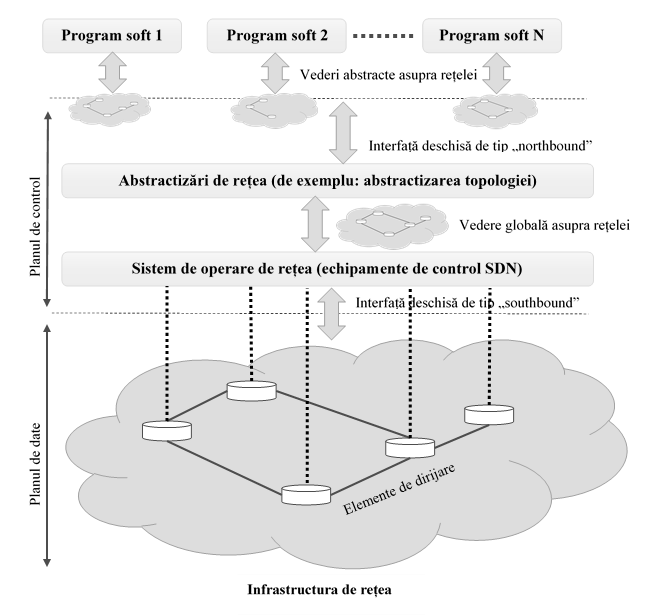
\includegraphics[width=1\textwidth]{arhitectura_sdn}
	\caption{Arhitectura SDN și abstractizările fundamentale~\cite{kreutz2015software}}
	\label{fig:arhitectura_sdn}
\end{figure}

În mod ideal, \textit{abstractizarea dirijării} reprezintă permiterea oricărui comportament de dirijare dorit de aplicațiile software din rețea (cu ajutorul planului de control),  fără a necesita cunoașterea detaliilor legate de capabilitățile hardware ale infrastructurii existente. Un exemplu pentru o astfel de abstractizare este protocolul OpenFlow.

\textit{Abstractizarea distribuției} se referă la faptul că aplicațiile \gls{sdn} nu ar trebui să cunoască problemele stărilor distribuite din rețea, transformând problemele unui plan de control distribuit, cum era în rețelele tradiționale, într-un plan de control logic centralizat. Acesta este realizat printr-un nivel comun de distribuţie, în \gls{sdn} fiind reprezentat de sistemul de operare de rețea. Acesta are două mari funcții: instalarea comenzilor de control pe echipamentele de dirijare și colectarea de informaţii despre starea planului de date, pentru a putea oferi programelor software o vedere de ansamblu asupra rețelei.

\textit{Abstractizarea specificărilor} reprezintă capabilitatea unui program software din rețea de a exprima un anume comportament al acesteia fără a fi responsabil personal și de implementarea acestui comportament. Acest lucru se poate realiza prin soluții de virtualizare, precum și cu ajutorul limbajelor de programare de rețea.

Arhitectura \gls{sdn} poate fi privită ca o structură cu mai multe niveluri, având fiecare funcțiile sale specifice. Unele niveluri sunt necesare în orice implementare \gls{sdn}, în timp ce altele pot fi prezente doar în anumite implementări particulare. Aceste niveluri sunt ilustrate în Figura \ref{fig:niveluri_sdn} și vor fi prezentate în continuare \cite{kreutz2015software}.

\begin{figure}[h]
	\centering
	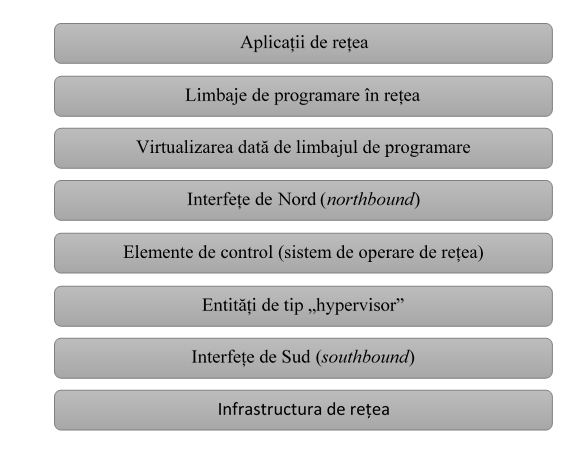
\includegraphics[width=1\textwidth]{niveluri_sdn}
	\caption{Nivelurile rețelelor definite prin software}
	\label{fig:niveluri_sdn}
\end{figure}


\paragraph{Nivelul 1: Infrastructura}

Infrastructura pentru o rețea definită prin programe software este compusă, la fel ca în cazul rețelelor tradiționale, din echipamente de rețea (comutatoare, rutere, echipamente de transport de date etc.). Însă, diferenţa majoră constă în faptul că, în \gls{sdn}, echipamentele de rețea sunt simple elemente de dirijare de trafic, inteligenţa lor fiind mutată în echipamentele de control \gls{sdn} și în aplicațiile software. O altă diferenţă importantă este aceea că echipamentele care constituie infrastructura de rețea trebuie să implementeze interfețe standard (cum ar fi OpenFlow), care să asigure compatibilitatea comunicației și a configurărilor, dar și interoperabilitatea cu alte echipamente, atât din planul de control cât și din cel de date, indiferent de producător. Acest lucru era destul de dificil în rețelele tradiționale, din cauza multitudinii de interfețe proprietare.

În paradigma \gls{sdn}, elementele care alcătuiesc infrastructura rețelei nu mai iau deciziile de dirijare pe baza adresei destinație, ca în cazul rețelelor tradiționale, ci pe baza unor fluxuri de date \cite{mckeown2008openflow}. Presupunând o rețea bazată pe protocolul OpenFlow, elementele de dirijare se bazează pe o secvenţă de tabele de fluxuri, unde fiecare intrare din tabel conţine: (i) o regulă de asociere, (ii) acțiunile care trebuie executate asupra pachetelor care se potrivesc regulii și (iii) contoare care să menţină o statistică despre pachetele care s-au potrivit. Prioritatea regulilor este dată de ordinea din tabelul de fluxuri. Acțiunile posibile asupra pachetelor pot fi: dirijarea acestora către un port de ieșire, dirijarea către echipamentul de control, aruncarea pachetelor, trimiterea către secvența normală de prelucrare, trimiterea către următorul tabel de fluxuri etc. Regulile de potrivire care se pot aplica pachetelor se pot baza pe mai multe câmpuri din antetul pachetului, cum ar fi câmpuri de nivel doi (Ethernet), MPLS, de nivel 3 (IPv4/v6), câmpuri de nivel 4 (TCP/IP) etc., în aproape orice fel de combinație.

\paragraph{Nivelul 2: Interfețele de Sud (\textit{southbound})}

Interfețele de Sud fac legătura între echipamentele de dirijare și echipamentele de control din rețea, îndeplinind astfel una dintre funcțiile de bază ale rețelelor definite prin programe soft: separarea planurilor de date și de control. Terminologia Nord/Sud se raportează la controlerul \gls{sdn}.

Acest tip de interfețe este foarte bine privit de către industrie. Prin standardizarea acestora se va permite construirea de rețele cu echipamente care să poată proveni de la mai multi producători, promovând astfel interoperabilitatea.

Cel mai acceptat și utilizat standard pentru acest tip de interfețe este OpenFlow. Acesta propune specificaţii comune pentru implementarea canalului de comunicaţie dintre echipamentele de dirijare și cele de control. Protocolul OpenFlow furnizează trei surse de informații pentru sistemul de operare de rețea: (i) mesaje bazate pe evenimente, care sunt trimise de echipamentele de dirijare către cele de control în momentul în care apare o schimbare a legăturii de date sau a unui port; (ii) statistici despre fluxurile de date, care sunt generate în echipamentele de dirijare și trimise către echipamentele de control; (iii) mesaje care conţin și pachete de date și sunt trimise de către echipamentele de dirijare către cele de control în momentul în care nu ştiu cum să trateze un anumit tip de flux de date sau din cauza faptului că există o acțiune explicită de tipul \textit{trimite la echipamentul de control} în tabela de fluxuri. Aceste tipuri de informații sunt esențiale pentru furnizarea de detalii despre fluxurile de date sistemului de operare de rețea.

Deşi este cel mai utilizat protocol, OpenFlow nu este singura interfață de Sud pentru rețelele definite prin programe soft. Există și alte propuneri pentru acest tip de interfețe, dintre care amintim: \gls{netconf}, \gls{forces}, OpFlex, \gls{pof}, \gls{ovsdb}, \gls{rofl}, \gls{hal}, OpenState etc. \cite{haleplidis2015network, zhou2014research, onfts016}.

\paragraph{Nivelul 3: Entitățile de tip \textit{hypervisor} de rețea}

Entităţile de tip \textit{hypervisor} reprezintă o soluție software, firmware, sau hardware care creează și rulează mașini virtuale. Acestea permit unor mașini virtuale distincte să partajeze aceleași resurse hardware. Astfel au apărut noi modele de afaceri și tehnologii, cum ar fi aplicațiile de tip cloud, unde fiecare utilizator poate avea resursele sale virtuale, de la puterea de calcul până la spaţiul de stocare. Din păcate, acest model nu a putut fi aplicat și pentru resursele de rețea, acestea fiind configurate în continuare în mod static și independent una față de cealaltă.

Există două cerinţe ale aplicațiilor de la rețea: spaţiul de adresare și topologia rețelei. Volume diferite de muncă necesită diferite servicii și topologii de rețea, însă acestea sunt greu de oferit de către o singură topologie fizică. De asemenea, aplicațiile care rulează într-un mediu virtualizat funcționează în același spațiu de adresare ca infrastructura fizică. Astfel, mașinile virtuale nu pot migra în locuri arbitrare, deoarece schema de adresare este fixă și greu de modificat.

Soluția la această problemă ar fi ca rețeaua să ofere la rândul ei virtualizare, din punctul de vedere al topologiei și al spațiului de adresare. Apoi, fiecare aplicație care rulează într-o mașină virtuală ar avea posibilitatea să configureze atât nodurile de calcul cât și rețeaua, în același timp. Acest lucru nu este posibil prin tehnologiile actuale, cum ar fi \gls{vlan} - domeniu virtualizat de nivel 2, \gls{nat} - spațiu de adresare IP virtualizat și \gls{mpls} - rute virtuale, deoarece rețeaua nu se poate reconfigura într-un mod global, fiind nevoie ca fiecare element de rețea să fie reconfigurat individual \cite{kreutz2015software, peng2012vdn, koponen2014network}.

Rețelele definite prin software încearcă să ofere posibilitatea de virtualizare a rețelei, prin această entitate de tip \textit{hypervisor}. Există mai multe propuneri în acest sens, dintre care amintim: FlowVisor, \gls{nvp}, FlowN, RadioVisor, IBM SDN VE, OpenVirteX, HyperFlex, \gls{xdpd} etc. \cite{sherwood2009flowvisor, gudipati2014radiovisor, al2014openvirtex, sune2013xdpd, blenk2015hyperflex}.

\paragraph{Nivelul 4: Echipamentele de control / Sistemul de operare de rețea}

Sistemele de operare tradiționale oferă abstractizări pentru accesarea resurselor hardware, pentru administrarea accesului concurent la resurse și pentru a oferi mecanisme de securitate și protecție. Prin contrast, rețelele au fost administrate și configurate până acum cu ajutorul unor instrucțiuni de nivel jos, specifice fiecărui echipament și cu sisteme de operare de rețea proprietare (cum ar fi IOS de la Cisco sau JunOS de la Juniper). Acestea nu furnizează abstractizări care să ofere, într-un mod transparent, funcționalități de bază \cite{kreutz2015software}.

În cadrul \gls{sdn} se încearcă găsirea unor soluții în acest sens, printr-un control logic centralizat, oferit de un sistem de operare de rețea. Acesta va trebui să ofere abstractizări, care să fie apoi folosite de dezvoltatorii de aplicații software. Printre serviciile oferite de sistemul de operare de rețea ar trebui să se regăsească funcționalități generale, cum ar fi: descoperirea dispozitivelor de rețea, distribuirea configuraţiei rețelei, starea rețelei sau informații despre topologia rețelei.

Echipamentul de control este elementul critic din arhitectura \gls{sdn}, deoarece el va trebui să interpreteze aplicațiile dezvoltate pentru administrarea rețelei și să genereze configurația acesteia pe baza politicilor definite acolo. Există deja o multitudine de echipamente de control propuse pentru a fi utilizate în arhitectura \gls{sdn}, diferite în foarte multe aspecte. Unul dintre cele mai importante, care diferențiază echipamentele de control, este tipul arhitectural folosit: centralizat sau distribuit \cite{dixit2013towards, levin2012logically, jimenez2014controller}.

Un echipament de control centralizat reprezintă o entitate care administrează toate dispozitivele din planul de date al rețelei \cite{ome2012software}. În mod natural, acesta poate fi privit ca un punct unic de defectare a rețelei și ar putea aduce limitări în extensibilitatea acesteia, deoarece este posibil ca un singur echipament de control să nu fie suficient pentru administrarea unui număr mare de echipamente de dirijare. Printre propunerile de astfel de echipamente de control se numără: Maestro, Beacon (care poate administra un număr foarte mare de fluxuri de date, undeva la 12 milioane de fluxuri pe secundă, conform~\cite{erickson2013beacon}), NOX-MT, sau Floodlight. Acestea se bazează pe mai multe fire de execuție și pe paralelismul oferit de arhitecturile de calculatoare cu mai multe nuclee.

Pe de altă parte, un sistem de operare de rețea distribuit poate rezolva problema extensibilităţii rețelei, fiind potrivit pentru orice tip de rețea. Această distribuţie poate fi realizată printr-un grup de echipamente de control care să se afle în același loc, sau printr-un set de dispozitive distribuite fizic în mai multe locuri. Această ultimă variantă ar putea fi mai potrivită pentru prevenirea diferitelor defecţiuni logice sau fizice. Câteva exemple de astfel de echipamente de control distribuite: Onix \cite{koponen2010onix}, HP VAN SDN, PANE, HyperFlow \cite{tootoonchian2010hyperflow}, \gls{onos}~\cite{berde2014onos} sau \gls{odl}~\cite{medved2014opendaylight}, SMaRtLight \cite{botelho2014smartlight} etc.

Însă, în cazul echipamentelor de control distribuite, apare o problemă destul de importantă: consistenţa datelor. Toate echipamentele de control ar trebui să citească aceeaşi valoare imediat după ce aceasta a fost scrisă, pentru a evita cazul când dispozitivele de control au imagini diferite asupra rețelei. Majoritatea propunerilor de până acum oferă doar o \textit{consistență scăzută}, ceea ce înseamnă că, după ce o valoare a fost scrisă într-un nod de control, valoarea se va reflecta, \textit{la un moment dat}, în toate nodurile de control. Acest lucru implică o perioadă de timp în care dispozitivele de control au viziuni diferite asupra rețelei. Există și propuneri de echipamente de control care oferă o \textit{consistență ridicată} (Onix și SMaRtLight) \cite{koponen2010onix, botelho2014smartlight}, care garantează citirea aceleiaşi valori de către orice nod de control, imediat după scrierea acesteia.

Există și situaţii unde o abordare hibridă ar fi cea mai potrivită, o arhitectură în care să existe grupuri de echipamente de control într-o parte de rețea și dispozitive de control distribuite în alte locuri din rețea.

\paragraph{Nivelul 5: Interfețe de Nord (\textit{northbound})}

Interfețele de Nord, împreună cu cele de Sud constituie cele mai importante două abstractizări din arhitectura rețelelor definite prin software. Dacă cele din urmă asigură comunicaţia dintre echipamentele de control și dispozitivele din planul de date al rețelei, fiind astfel mai mult orientate spre hardware, interfeţele de Nord alcătuiesc, în mare parte, un ecosistem software. Încă nu există un astfel de tip de interfețe care să fie acceptat la scară largă, cum este OpenFlow în cazul celor de Sud, însă acest lucru se va întâmpla probabil, pe măsură ce paradigma \gls{sdn} se va maturiza și cazurile de utilizare ale acestui tip de arhitectură de rețea se vor contura mai exact.

Este nevoie ca acest tip de interfețe să fie deschise și standardizate, astfel încât să se asigure interoperabilitatea și portabilitatea programelor soft pe mai multe tipuri de dispozitive de control. Un exemplu în acest sens îl constituie NOSIX~\cite{wundsam2012nosix}. Aceasta este o propunere, care poate fi comparată cu standardul \gls{posix} din sistemele de operare și care oferă abstractizări ce garantează independenţa față de limbajul de programare și dispozitivul de control folosite \cite{barney2009posix}. Dintre celelalte propuneri de interfețe de Nord amintim: RESTCONF, SFNet, Pyretic, NetCore, Frenetic, Nettle etc. \cite{bierman2017restconf, yap2010towards, reich2013modular, monsanto2012compiler}.

\paragraph{Nivelul 6: Virtualizarea dată de limbajul de programare}

Există două caracteristici principale ale soluţiilor de virtualizare date de limbajele de programare: permiterea mai multor niveluri de abstractizare, concomitent cu oferirea proprietăţilor dorite, cum ar fi protecţia și abilitatea de a exprima modularitatea.

Metodele de virtualizare pot permite, de exemplu, diferite imagini asupra unei singure infrastructuri fizice de rețea. Un \textit{comutator virtual} ar putea reprezenta o combinație de mai multe dispozitive de dirijare. Acest mod de lucru simplifică sarcinile dezvoltatorilor de aplicații, care nu trebuie să ţină cont individual de elementele de rețea care alcătuiesc acel \textit{comutator virtual}. Dezvoltarea și implementarea unor aplicații de rețea complexe este simplificată cu ajutorul acestor abstractizări.

O altă formă de virtualizare dată de limbajul de programare o reprezintă împărţirea statică a rețelei în secţiuni. Acest lucru se face de către compilator, bazat pe definiţiile date de nivelul aplicație. După compilare va rezulta un program unitar de control, care are deja implementate funcțiile pentru împărțirea rețelei în bucăţi și comenzile de configurare a acestora. În acest caz nu mai este nevoie de entitatea \textit{hypervisor} care să administreze dinamic bucăţile de rețea.

Există diverse propuneri pentru astfel de soluții de virtualizare, cum ar fi: Pyretic, Splendid, libNetVirt, FlowVisor, IBM SDN VE etc. \cite{reich2013modular, schlesinger2012splendid, turull2012libnetvirt, sherwood2009flowvisor}.

\paragraph{Nivelul 7: limbaje de programare în rețea}

Limbajele de programare au evoluat de la limbaje mașină, specifice hardware-ului, cum era limbajul de asamblare pentru arhitecturile x86, până la limbaje de nivel înalt, cum ar fi Java sau Python. În același mod, limbajele de programare folosite în programarea rețelelor evoluează de la OpenFlow (echivalentul limbajului de asamblare) la limbaje de nivel înalt, cum ar fi Pyretic, Procera, NetCore, Frenetic etc. \cite{reich2013modular, voellmy2012procera, monsanto2012compiler}.

Aceste limbaje de programare de nivel înalt oferă câteva avantaje în contextul rețelelor definite prin software: facilitează dezvoltarea virtualizării rețelei, creează abstractizări care simplifică programarea elementelor de dirijare, promovează modularizarea software și reutilizarea codului în planul de control și chiar îmbunătăţesc dezvoltarea și inovația prin crearea unor medii de lucru mai productive.

Există două tipuri de paradigme de programare în contextul \gls{sdn}: cea declarativă, care este cea mai răspândită și cea imperativă, care este reprezentată doar prin limbajul Pyretic. Paradigma declarativă reprezintă o abordare în care rețelei i se spune ce tip de comportament să aibă și aceasta se va configura (luând singură decizii) astfel încât să îndeplinească acea cerinţă. Paradigma imperativă se referă la situația în care programatorul îi spune rețelei cum să acţioneze și rezultatul va fi cel așteptat, fără ca aceasta să ia propriile decizii.

Scopul \gls{sdn} este ca, în final, să ofere facilități de administrare a rețelelor pe baza infrastructurii definite anterior. Cu ajutorul progreselor din domeniul limbajelor de programare de nivel înalt se va facilita crearea unui ecosistem propice pentru dezvoltarea aplicațiilor \gls{sdn}.

\paragraph{Nivelul 8: Aplicațiile de rețea}

Aplicațiile software vor reprezenta cea mai importantă parte a rețelelor definite prin software, deoarece acestea vor implementa logica de control, care va fi translatată în comenzi ce vor fi instalate la nivelul dispozitivelor din planul de date.

Majoritatea aplicațiilor software din cadrul \gls{sdn} se încadrează într-una din următoarele cinci categorii, conform~\cite{kreutz2015software}: ingineria traficului, securitate și fiabilitate, măsurători și monitorizare, reţelistica centrelor de date, mobilitate și rețele fără fir.

Programele software din categoria mobilitate și microunde își propun să faciliteze implementarea și administrarea rețelelor fără fir, cum ar fi rețelele locale fără fir - \gls{wlan} sau rețelele de telefonie mobilă. Un plan de control distribuit, cum există în momentul de față în rețelele fără fir, nu este optim pentru implementarea mecanismelor de transfer dintre celule, pentru micșorarea interferențelor, pentru alocarea resurselor radio, pentru administrarea spectrului limitat de frecvenţe etc. Aceste probleme sunt adresate în \gls{sdn} și se pot rezolva mai uşor cu ajutorul acestei noi paradigme.

\section{Standardizarea SDN}

Activitățile de cercetare și standardizare din jurul \gls{sdn} au loc pe două planuri importante. Pe de o parte, există organizaţiile care dezvoltă standarde - \gls{sdo}, care sunt formate din reprezentanţi ai industriei, ai academiei, sau alte entități și au ca scop dezvoltarea de specificaţii sau recomandări tehnice, în contextul \gls{sdn} care să fie folosite de toată industria rețelisticii. Autorii din~\cite{schneider2014standardizations} amintesc astfel de organizații: \gls{onf}, \gls{ietf}, \gls{etsi}, \gls{itu-t}, \gls{ieee}. 

Pe de altă parte, există asociații sau comunități de oameni, în general care fac parte din industrie, ale căror rezultate ale cercetării candidează pentru a deveni standarde. Aceste rezultate sunt, de obicei, implementări cu sursă deschisă ce vor fi folosite ulterior în industrie. Exemple de astfel de comunități sunt prezente în~\cite{halpern2014standards, meyer2013software}: OpenDaylight (activităţi ce se desfăşoară sub patronajul fundaţiei Linux), \gls{mef}, \gls{bbf}, \gls{oif}.

Activitățile de standardizare ale \gls{sdn} sunt foarte importante, asigurându-i acestei tehnologii o evoluţie stabilă și aducând-o la o maturitate care îi va permite adoptarea pe scară largă în industria rețelisticii, mitigând astfel dezavantajele rețelelor tradiționale.

Sunt mai multe planuri pe care se lucrează pentru standardizarea \gls{sdn}. Unul dintre aceste planuri este cel al interfeţelor de Sud, care fac legătura între echipamentele de dirijare și echipamentele de control \gls{sdn}. Protocolul OpenFlow este un exemplu în acest sens, însă nu este singurul protocol capabil să facă legătura între planurile de date și de control. În ultimul timp se pune foarte mare accent pe \gls{netconf} ca o alternativă pentru a configura echipamentele care dirijează traficul, după cum se poate observa în~\cite{csoma2015escape, felix2014multi, zhou2014research}. Astfel apare nevoia de a dezvolta modele informaţionale care să abstractizeze echipamentele din planul de date și care să poată fi folosite de \gls{netconf} pentru a configura dispozitivele. Și planul interfeţelor de Nord are un rol important în standardizare, deoarece poate oferi un punct de plecare comun pentru dezvoltatorii de aplicații \gls{sdn}. De exemplu, în cadrul \gls{onf} există un grup care se ocupă cu activităţi de standardizare în această direcţie. Un alt plan este reprezentat de implementările software, cu sursă deschisă (\textit{open-source}), care se crează în acest context. Așa cum evidenţiază și autorii din~\cite{lin2014software, rothenberg2014open}, aceste implementări sunt foarte importante prin ecosistemele care apar ca urmare a activităţii comunităţilor care dezvoltă software cu sursă deschisă.

O importanţă foarte mare în cadrul acestor activităţi o au și demonstraţiile de concept. Acestea au capacitatea de a demonstra avantajele pe care \gls{sdn} le aduce nu doar la un nivel teoretic, ci într-un mod practic, propunând diferite cazuri reale de utilizare a acestei tehnologii și aplicând-o, într-un mod restrâns, unor topologii formate din echipamente reale. Scopul acestora este, pe de o parte, de a adăuga un plus de valoare activităţilor de standardizare și de a testa și proba rezultatele acestor activităţi. Pe de altă parte, aceste demonstraţii de concept au scopul de a atrage atenţia și altor entități din industrie și a duce la înlesnirea adoptării acestei tehnologii pe scară largă.

\subsection{Open Networking Foundation}

\gls{onf} este o organizaţie non-profit formată din peste două sute de membri care fac parte din industrie, academie, sau institute de cercetare, ce are ca obiectiv accelerarea adoptării \gls{sdn} pe scară largă in industria rețelisticii prin dezvoltarea de standarde deschise și de ecosisteme software cu sursă deschisă. \gls{onf} a apărut ca urmare a activităţii de cercetare din jurul protocolului OpenFlow din cadrul Universităţii Stanford. Dintre membrii cei mai importanţi amintim operatori de rețele, precum AT\&T, Google, Facebook, Verizon, Deutsche Telekom sau Telefonica, producători de echipamente, cum ar fi Cisco, Ericsson, Huawei, Intel sau NEC și reprezentanţi ai unor universităţi cunoscute, ca Stanford sau Princeton.

Activitățile din cadrul \gls{onf} sunt împărţite în mai multe zone de interes, conform \cite{onftech}:
\begin{itemize}
	\item \textit{Operatori}. Această zonă se ocupă de mai multe aspecte, precum \gls{sdn} în contextul sistemelor de tip Purtător - \textit{Carrier Grade} - (rețelele de telecomunicaţii foarte sigure, cu o disponibilitate de peste 99,999\% și recuperare în caz de defectare de sub 50 de milisecunde), în centre de date, în întreprinderi sau aspecte legate de migrarea serviciilor dintr-o rețea tradiţională într-o rețea definită prin software.
	\item \textit{Servicii}. Se ocupă de proiecte care permit existența aplicațiilor și serviciilor de rețea care au la bază tehnologia \gls{sdn}. Astfel, există mai multe grupuri de lucru care analizează arhitectura \gls{sdn} și modul în care aceste principii se aplică în imaginea de ansamblu a unei rețele de comunicaţii, un model informaţional \textit{de bază}, care să reprezinte piatra de temelie cu ajutorul căreia să se dezvolte alte modele informaţionale, specializate pentru anumite aplicații sau tehnologii, interfeţele de Nord, pentru a facilita dezvoltarea aplicațiilor \gls{sdn}, probleme de securitate pe care această nouă tehnologie le poate întâmpina.  
	\item \textit{Specificaţii}. Zonă care are ca responsabilitate publicarea tuturor specificaţiilor și recomandărilor tehnice create de \gls{onf}. Acestea includ protocoalele OpenFlow, OF-Config dar și alte interfețe standard care se dezvoltă pentru tehnologii de transport de diferite tipuri (optic, fără fir). Există și un proiect care se ocupă de testare și interoperabilitate, scopul acestuia fiind accelerarea adoptării protocolului OpenFlow prin certificări și promovarea interoperabilităţii între diferiţi producători de echipamente \cite{onftr539}.
	\item \textit{Piaţă}. Această zonă se concentrează pe educarea comunităţii \gls{sdn} în legătură cu valoarea pe care standardele \gls{onf} le oferă rețelelor definite prin software și promovarea adoptării unor astfel de rețele definite prin software cu sursă deschisă. Aceste obiective sunt îndeplinite prin publicaţii, evenimente care se organizează sau demonstraţii care să arate comunităţii cazuri reale de utilizare.
\end{itemize}

Există trei tipuri de publicaţii care reies din activitățile \gls{onf}: (i) \textit{specificaţii}, care includ toate standardele care definesc un protocol, modelul informaţional, funcționalități și documente despre cadrele asociate; publicaţiile normative astfel rezultate se numesc Specificaţii Tehnice - \gls{ts} și sunt supuse unor procese de licenţiere; (ii) \textit{recomandări}, care includ consideraţii arhitecturale, cazuri de utilizare, analiza cerințelor, terminologie; aceste documente referă documente normative \gls{onf}, dar nu necesită licenţiere și pot fi utilizate în mod liber, având rolul de Recomandări Tehnice - \gls{tr}; (iii) \textit{publicaţii}, reprezentând documente care conţin informații ce ajută în procesele de lansare a \gls{sdn} în producție, rezumate ale soluţiilor, studii de caz sau cărţi albe (\textit{white papers}); aceste documente nu au caracter normativ și pot fi folosite în mod liber.

În continuare vor fi enumerate câteva astfel de documente produse de către \gls{onf}: \textit{OpenFlow Switch Specification Ver. 1.5.1} (TS-025), care descrie cerinţele unui comutator logic ce suportă protocolul OpenFlow; \textit{OpenFlow Management and	Configuration Protocol 1.2 (OF-Config 1.2)} (TS-016), document ce descrie motivația, cerințele, scopul și specificaţiile protocolului OF-Config; \textit{Conformance Test Specification for OpenFlow Switch Specification V1.3.4} (TS-026), definind cerinţele și procedurile de test care determină conformitatea unui comutator cu specificațiile protocolului OpenFlow 1.3.4; \textit{Core Information Model (CoreModel) 1.2} (TR-512), care prezintă modelul informațional de bază, pe care celelalte modele informaționale dezvoltate în \gls{onf} se bazează; \textit{Microwave Information Model} (TR-532), reprezentând modelul informațional ce descrie echipamentele de transport de date fără fir. Aceste ultime două documente vor fi detaliate în următorul capitol, fiind baza dezvoltării și implementării simulatoarelor propuse în această lucrare.

Un rol important în adoptarea \gls{sdn} de către operatori și în diseminarea rezultatelor din cadrul \gls{onf} îl au demonstraţiile de concept. Acestea adună laolaltă operatori, producători de echipamente și integratori de servicii, cu scopul de a demonstra recomandările produse de activitatea de cercetare. În contextul rețelelor de transport de date fără fir, proiectul \gls{wt}, care face parte din grupul \gls{otwg}, a terminat cu succes patru astfel de demonstraţii de concept~\cite{onf2015_poc1, onf2016_poc2, onf2016_poc3, onf2017_poc4}.

Prima astfel de demonstraţie a avut loc în octombrie 2015, în Madrid și a fost organizată de Telefonica, împreună cu Universitatea Carlos III. Scopul acesteia a fost de a extinde protocolul OpenFlow cu atribute specifice echipamentelor de transport de date fără fir. Astfel, interfaţa de Sud folosită a fost OpenFlow, în timp ce echipamentul de control \gls{sdn} a fost \gls{onos}. Au fost prezentate două cazuri de utilizare: (i) pornirea/oprirea unei interfeţe radio în funcţie de nivelul de trafic ce trebuie transmis de către echipament, economisind astfel energie în momentele în care nivelul de trafic în reţea nu este foarte ridicat; (ii) schimbarea căilor de date într-un ruter, în cazul în care se pierd pachete pe legătura radio, ca urmare a unor schimbări meteorologice (simulate prin folosirea unui atenuator variabil pe legătura radio).

A doua demonstraţie de concept a avut loc în aprilie 2016, la München și a fost organizată de Telefonica. Spre deosebire de prima demonstraţie, în cea de-a doua s-a folosit drept interfaţă de Sud protocolul \gls{netconf}, iar echipamentul de control \gls{sdn} a fost \gls{odl}. Ca model informaţional YANG pentru configurarea echipamentelor s-a ales un model pentru microunde simplificat (conţinea un număr limitat de atribute). Acesta a fost dezvoltat de către grup și apoi implementat de către echipamentele de la diferiţi producători. Au fost demonstrate mai multe cazuri de utilizare folosind aplicaţii \gls{sdn} care se bazează pe acel model: detectarea și configurarea de noi echipamente, detectarea și corecţia (printr-o acţiune a operatorului) diferenţelor între configuraţia curentă și cea planificata, detecţia și vizualizarea reţelei de transport configurate, primirea, afişarea și stocarea evenimentelor și alarmelor din reţea.

Cea de-a treia demonstraţie de concept s-a desfăşurat în octombrie 2016 și a avut loc în centrul de cercetare WINLAB de la Universitatea Rutgers, fiind organizat de AT\&T. S-au ales aceeaşi interfaţă de Sud și acelaşi echipament de control \gls{sdn}, scopul acestei demonstraţii fiind de a proba utilitatea întregului model informaţional pentru microunde (conţinea toate atributele pe care le poate avea un echipament de transport de date fără fir). S-a implementat și modelul de bază (\textit{Core Model}), dezvoltat de alt grup din cadrul \gls{onf}. Au fost demonstrate aplicaţiile dezvoltate pentru cea de-a doua demonstraţie, dar și două noi aplicaţii: una care administrează spectrul, prin compararea și configurarea frecvenţelor planificate și cele configurate pe echipamente, realocându-le în caz că nu se potrivesc; cealaltă, denumită automatizarea în bucla închisă, demonstra un răspuns simplist la anumiţi factori declanşatori (interni, externi sau temporali).

A patra demonstraţie de concept a avut loc în iunie 2017, la Bonn și a fost organizată de Deutsche Telekom. S-au folosit mai multe modele informaţionale: modelul pentru microunde, modelul de bază, un model Ethernet simplificat și un model pentru sincronizare - pentru \gls{ptp}, plecând de la un model dezvoltat de ITU-T. Astfel, s-au putut demonstra mai multe cazuri de utilizare: administrarea echipamentelor care transportă date fără fir, administrarea indicatorilor de performanță ai echipamentelor, administrarea puterii echipamentelor, administrarea echipamentelor capabile Ethernet, recalcularea căilor de trafic Ethernet într-o rețea sau administrarea echipamentelor care suportă \gls{ptp}. 

\subsection{IETF}

Un alt \gls{sdo} care prestează activităţi de standardizare în domeniul rețelelor definite prin software este \gls{ietf}. Această organizaţie, în general, oferă standardele de bază folosite în Internet. Obiectivul lor declarat este îmbunătăţirea funcţionării Internetului prin dezvoltarea de documente tehnice relevante și de înaltă calitate care să ghideze proiectarea, utilizarea și administrarea Internetului.

Doar puține din grupurile de lucru din cadrul \gls{ietf} se ocupă cu activităţi care au legătură cu tehnologia \gls{sdn}. Unul dintre acestea a dezvoltat \gls{forces}, iniţiativă ce separa planurile de date și de control ale echipamentelor \cite{doria2010forwarding}, cu câțiva ani înainte ca protocolul OpenFlow, mult mai cunoscut, să propună asta într-un mod care să permită o adoptare mai rapidă în industrie.

Alt grup de lucru se ocupă de \textit{interfaţa către sistemul de rutare} - \gls{i2rs}. Acesta își propune să dezvolte interfețe pentru ca aplicațiile \gls{sdn} să poată accesa sistemul de rutare al rețelei. Se doreşte ca beneficiarii \gls{i2rs} să fie aplicații de administrare, echipamente de control \gls{sdn} sau aplicații de utilizator care au cereri specifice la adresa rețelei. Acestea ar permite informaţiilor, politicilor și parametrilor operaţionali să fie introduşi sau extraşi din sistemul de rutare, fără a afecta consistenţa datelor și coerenţa infrastructurii de rutare. Această abordare poate fi privită ca un rival al protocolului OpenFlow, cu menţiunea că se aplică doar de la nivelul 3 în sus, în stiva OSI.

În interiorul grupului de lucru \gls{spring} se discută un control al rutării care să permită indicarea unei căi de dirijare încă de la sursa de trafic \cite{schneider2014standardizations}, calcularea acesteia putând fi făcută atât centralizat, cât și distribuit. Tot în cadrul \gls{ietf} se dezvoltă și protocolul \gls{netconf}, însă acesta va fi detaliat într-o secţiune viitoare.

Parte din \gls{ietf} este și \gls{irtf}. Aceasta este o organizaţie paralelă, care se ocupă mai mult de partea de cercetare, sprijinind proiectele care se crede că vor fi benefice comunităţii Internetului, dar care nu sunt încă pregătite pentru implementare. Aici există un grup de lucru care investighează tehnologia \gls{sdn} din mai multe perspective, cu scopul de a recunoaşte atât abordări ce pot fi definite și lansate pe termen scurt, dar și provocări viitoare: \gls{sdnrg}. Sunt de interes probleme ca extensibilitatea soluţiei, abstractizări sau limbaje de programare ce pot fi folosite în contextul \gls{sdn}. Se doreşte ca acest grup să ofere un spațiu comun tuturor cercetătorilor cu interes în acest domeniu.

%\subsection{ETSI}
%
%Unul dintre grupurile specificaţiilor pentru industrie din cadrul \gls{etsi} se numeşte grupul \gls{nfv}. Conceptul de virtualizare a funcţiilor de rețea este unul complementar rețelelor definite prin software. Este o iniţiativă a operatorilor de rețea și are ca scop să permită acestora să profite de noile tehnologii ce apar, să le crească abilităţile de a livra servicii, să reducă costurile și să crească viteza de lansare în producție a serviciilor noi sau experimentale.
%
%Chiar dacă accentul este pus pe virtualizarea funcţiilor de rețea, a fost foarte bine înţeles faptul că utilizarea tehnologiei \gls{sdn} reprezintă un avantaj major și că multe dintre cazurile de utilizare propuse pot fi implementate folosind această paradigmă. Astfel, grupul lucrează la standardizare și stabileşte protocoale împreună cu celelalte organizaţii care se ocupă de standardizarea \gls{sdn}.
%
%\subsection{ITU-T}
%
%Unul dintre cele mai vechi organizaţii de standardizare, \gls{itu-t}, a avut o importanţă majoră în multe aspecte critice din domeniul telecomunicaţiilor. În contextul \gls{sdn}, grupul se ocupă de în principal de arhitectura și cerinţe pentru utilizarea acestei tehnologii în rețelele de transport de date. Deoarece acest tip de rețele au cerinţe importante, diferite de celelalte rețele, evidenţierea acestora de către \gls{itu-t} ajută la orientarea eforturilor de standardizare în direcţia corectă. 
%
%Zonele de interes pentru grupurile care fac parte din această organizaţie sunt: aspecte arhitecturale ale securităţii în \gls{sdn} și servicii pentru securitate prin \gls{sdn}, specificaţii pentru arhitectura planului de control în rețele de transport de date, cerinţe de semnalizare folosind tehnologia \gls{sdn} sau cerinţe funcţionale și arhitecturale pentru \gls{sdn} și rețelele viitorului.

\section{SDN în contextul reţelelor actuale}

Chiar dacă nu este o tehnologie ajunsă la maturitate în toate aspectele unei rețele, paradigma \gls{sdn} este deja folosită în rețele de producție de anumite tipuri. Autorii din \cite{alvizu2017comprehensive} evidenţiază faptul că evoluția \gls{sdn} este susţinută de către trei mari porţiuni ale industriei rețelisticii: furnizorii serviciilor de tip \textit{cloud} (care utilizează mari centre de date), furnizorii de servicii de telecomunicaţii și întreprinderile, așa cum se poate observa și în Figura \ref{fig:sdn_network_deployments}. 

\begin{figure}[h]
	\centering
	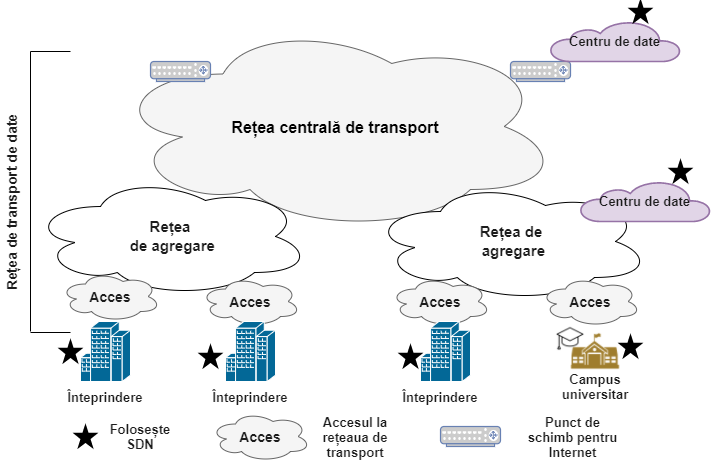
\includegraphics[width=1\textwidth]{sdn_network_deployments}
	\caption{Implementarea SDN în contextul rețelelor actuale~\cite{alvizu2017comprehensive}}
	\label{fig:sdn_network_deployments}
\end{figure}

Astfel, \gls{sdn} este implementat deja cu succes în rețelele unor campusuri universitare (Universitatea Stanford, de exemplu, dat fiind faptul că această paradigmă își are originile acolo), în mari centre de date sau în întreprinderi. În cazul rețelelor de transport, încă se duc activităţi de standardizare care să permită operatorilor rețelelor de telecomunicaţii să implementeze această tehnologie în cel mai scurt timp, beneficiind astfel de avantajele pe care aceasta le oferă (cel mai important, din punctul lor de vedere, fiind reducerea costurilor).

Această secţiune va prezenta în continuare utilizarea \gls{sdn} la momentul actual, în mai multe contexte actuale: în rețelele din marile centre de date, în rețelele de tip hibrid, care combină rețelele tradiționale cu \gls{sdn} sau prin studii de caz, implementări sau experimente efectuate pe teren (în rețele de producție).

\subsection{SDN în centrele de date}

Centrele de date reprezintă grupări de calculatoare cu putere mare de procesare și capacitate mare de stocare. Această idee nu este una nouă, fiind prezentă de câteva decenii, însă în timp au evoluat aceste caracteristici ale calculatoarelor, precum și numărul lor într-un centru de date. În zilele noastre acestea au ajuns sa conţină mii sau chiar zeci de mii de mașini fizice (servere) \cite{goransson2016software}.

Creșterea numărului de servere și a puterii de stocare, combinate cu creșterea vitezei și a lățimii de bandă din rețea a dus la dorința de a stoca din ce în ce mai multă informație în centre de date tot mai mari. În mod natural, acest lucru va însemna combinarea centrelor de date pentru a forma altele mai mari. Pe lângă acest aspect, se pune foarte mare accent în ultimul timp pe tehnologii de virtualizare, care permit unui server rularea mai multor mașini virtuale, pentru diferite aplicații sau servicii ale utilizatorilor.

A fost creat astfel un mediu dinamic, atât în cadrul centrelor de date, cât și între acestea. După cum este prezentat și în \cite{onf_openflow_backbone2012}, operații precum prevenirea sau recuperarea în caz de dezastru, sau balansarea încărcării severelor au nevoie de o creștere a traficului între centrele de date, lucru ce duce la o administrare complexa a acelei rețele.

Centrele de date sunt folosite și în cazul oferirii de servicii de virtualizare de servere. Operaţiunile într-un astfel de mediu implică lucrul cu mașini virtuale și, de cele mai multe ori, necesitatea migrării acestora între diferite mașini sau centre de date. Asta înseamnă că diferite aplicații sau servicii trebuie să aibă o vedere proprie asupra rețelei dintre servere, care este doar o vedere la nivel logic, în comparaţie cu rețeaua fizică existentă. Așa cum este prezentat și în \cite{nadeau2013sdn}, crearea de astfel de rețele logice se poate face si fără \gls{sdn}, prin metode folosite și în rețelele tradiționale, cum ar fi cu ajutorul unor \gls{vlan}-uri. Însă, în cazul centrelor de date foarte mari, acestea pot fi insuficiente. Cum ele pot fi exprimate într-un pachet Ethernet doar prin 12 biţi, numărul maxim de rețele virtuale este 4096. Apare astfel nevoia unor alte metode, care sunt însă mai complex de configurat.

O metodă pentru crearea de rețele logice care să fie prezentate unor aplicații sau servicii este chiar folosirea tehnologiei \gls{sdn}, făcând abstracţie de rețeaua fizică. În \cite{onf_openflow_backbone2012, onf_sdn_datacenter2013, liu2014sdn, munoz2015integrated} se prezintă diferite metode care pot fi aplicate în astfel de cazuri, sau care chiar au fost demonstrate.

Soluția \gls{sdn} a fost chiar aplicată în rețele de producție. Așa cum se explică în \cite{google_casestudy}, centrele de date ale Google folosesc deja această soluție, cu ajutorul protocolului OpenFlow. Există două laturi ale rețelei de arie largă - \gls{wan} folosită de Google: o parte legată la Internet, care conţine traficul utilizatorilor și o parte internă, care transportă traficul dintre centrele de date. Cele două au caracteristici diferite ale traficului și, implicit, nevoi diferite. În acea rețea internă a fost implementat \gls{sdn}, prin protocolul OpenFlow. Avantajele evidenţiate de Google includ o viziune de ansamblu asupra rețelei, un răspuns mai rapid la erori, timp mai scurt de implementare, actualizări mai rapide ale software-ului rețelei, fără pierdere de trafic sau existența unui mediu de test de mare fidelitate. Chiar dacă în 2012, atunci când a fost implementată această tehnologie în rețea, protocolul OpenFlow era încă la început și nu avea toate facilităţile pe care le oferă astăzi, Google a arătat încă de atunci că tehnologia \gls{sdn} poate fi folosită, aducând foarte multe avantaje, în multe cazuri de utilizare din industria rețelisticii.

\subsection{SDN în rețelele hibride}

Rețelele hibride reprezintă o combinație între rețelele tradiționale și \gls{sdn}, având scopul de a combina avantajele aduse de ambele, cât timp tehnologia \gls{sdn} nu este încă destul de matură și prezintă unele dezavantaje. Un alt motiv pentru apariția acestor rețele hibride este imposibilitatea de a schimba rețelele de producție într-un timp foarte scurt, în același timp asigurând și funcționarea acestora în parametrii agreaţi.

Autorii din \cite{vissicchio2014opportunities} prezintă oportunităţile și provocările aduse de o astfel de abordare. Ei propun patru modele ale rețelelor hibride: (i) rețele hibride bazate pe topologie, (ii) rețele hibride bazate pe servicii, (iii) rețele hibride bazate pe clase și (iv) rețele hibride integrate. Avantajele prezentate de aceste modele hibride sunt flexibilitatea, robusteţea, extensibilitatea, costuri mai mici ale implementării, date de faptul ca nu toată rețeaua este actualizată. Pe de altă parte, această abordare vine și cu dezavantaje, reprezentate de nevoia de a administra paradigme eterogene și garantarea faptului că interacţiunea dintre ele este benefică.

În \cite{hong2016incremental, levin2013toward, canini2016panopticon} se propun sisteme care să permită o implementare incrementală a \gls{sdn} în rețele de tip hibrid pentru rețele ale întreprinderilor și ale furnizorilor de servicii. Autorii evidenţiază faptul că implementarea directă, într-o rețea de producție a acestei noi tehnologii este imposibilă și ar conduce atât la probleme de implementare, cât și la probleme operaționale în rețea. Ei susţin că implementarea \gls{sdn} în puncte cheie ale rețelelor va aduce avantajele acestei tehnologii, fără nevoia de a înlocui toată rețeaua de la început. Pentru a determina aceste puncte cheie, autorii propun un \textit{planificator al implementării}, care să analizeze topologia de rețea, împreună cu informaţiile istorice despre trafic și constrângeri de resurse.

Lucrarea \cite{jin2015telekinesis} prezintă o altă abordare pentru aceste rețele hibride. Autorii propun un echipament de control al rețelei care să poată interacţiona atât cu echipamentele care folosesc un control centralizat, cât și cu cele care au un control distribuit. Controlarea echipamentelor vechi din rețea, care nu suportă protocolul OpenFlow se face chiar cu ajutorul acestuia. Astfel, dacă se vrea alterarea fluxului de date dintr-un echipament vechi, autorii propun folosirea unei extensii a OpenFlow, numită \textit{LegacyFlowMod}, care să instruiască un echipament OpenFlow să trimită un alt pachet special către echipamentul vechi, astfel încât acesta să își schimbe tabela de dirijare.

Autorii din \cite{caria2015divide, caria2016link} susţin de asemenea că o soluție hibridă este mai potrivită. Propun astfel folosirea unor rețele care să combine \gls{sdn} cu protocolul \gls{ospf}, păstrând avantajele date de acest protocol vechi de rutare, care a fost folosit cu succes câteva zeci de ani și, în același timp, aducând și câteva din avantajele propuse de \gls{sdn}.

\subsection{Studii de caz. Implementări. Experimente în rețele de producție}

Există numeroase studii de caz sau experimente în rețele de producție care demonstrează utilitatea \gls{sdn} și faptul că această tehnologie poate fi implementată cu succes în rețelele din zilele noastre.

În \cite{nec2012hospital} se prezintă soluţia implementată în rețeaua spitalului \textit{Kanazawa University}, din Japonia. S-a folosit tehnologia \gls{sdn}, cu ajutorul protocolului OpenFlow pentru a uşura munca de administrare a rețelei spitalului, care devenea din ce în ce mai complexă, pe măsură ce noi echipamente medicale trebuiau adăugate. Rețeaua, fiind operată de personalul spitalului, era vulnerabilă la erorile provocate de greşelile umane. Trebuia asigurată izolarea între anumite departamente ale spitalului, în unele cazuri, astfel că administrarea rețelei devenea greoaie. Cu ajutorul \gls{sdn} a fost creată o soluție în care infrastructura de rețea este uşor de administrat, prin aplicații software care rulează deasupra echipamentului de control \gls{sdn}, permiţând departamentelor crearea de rețele virtuale proprii, asigurând în același timp conectivitate între departamente. Astfel, rețeaua spitalului a devenit stabilă și pregătită pentru dezvoltările rapide care apar în industria medicală în zilele noastre.

Lucrarea \cite{bidkar2014field} ilustrează folosirea \gls{sdn} în cadrul unei rețele optice de transport a unui furnizor de servicii prin Ethernet. Autorii au implementat această tehnologie pentru oferirea de servicii în acea infrastructură de rețea. Obiectivele urmărite au fost simplificarea administrării rețelei și furnizarea de trafic, în funcție de serviciul solicitat (de exemplu, lățime de bandă la cerere).

În \cite{kalman2014applicability} se analizează posibilitatea folosirii tehnologiei \gls{sdn} în rețelele Ethernet industriale. Autorul evidenţiază punctele în care această tehnologie s-ar putea aplica în rețelele industriale și avantajele pe care o astfel de implementare le-ar aduce.

Autorii din \cite{kobayashi2014maturing} urmăresc evoluția implementărilor \gls{sdn} pornind de la nivelul unei rețele dintr-un simplu laborator din cadrul Universităţii Stanford și până la rețele de nivel naţional. Cu ajutorul acestor studii se evidenţiază compromisurile care apar în implementarea acestei noi tehnologii în rețele de producție. De exemplu, pentru o simplă rețea a unui campus universitar, un singur server poate susţine tot planul de control al rețelei, incluzând echipamentul de control și diferitele aplicații care rulează acolo pentru administrarea acesteia. Primele cazuri de utilizare demonstrate cu ajutorul \gls{sdn} au fost rutarea pe cea mai scurtă cale de nivel 2, învăţarea adreselor de nivel 2 - \gls{mac}, descoperirea topologiei cu ajutorul \gls{lldp} sau colectarea de statistici de la comutatoarele din rețea. Aceste experimente au relevat câteva aspecte importante pentru performanţelor rețelelor \gls{sdn}: timpul necesar configurării fluxurilor de date în rețea, numărul de intrări în tabelele de fluxuri ale comutatoarelor. De asemenea, este important ca un comutator să fie hibrid, adică să suporte atât protocolul OpenFlow, cât și pe cele tradiționale. O altă fază a experimentelor conduse de aceşti autori a constat în împărțirea infrastructurii de rețea în mai multe rețele logice destinate diferitor aplicații. 

Toate aceste experimente și studii de caz prezentate au avut la bază protocolul OpenFlow, ducând la evoluția acestuia. Acest lucru nu trebuie să ne ducă însă cu gândul că tehnologia \gls{sdn} înseamnă doar OpenFlow. După cum se va vedea în capitolele următoare, în special în cazul rețelelor de transport de date prin microunde, există și alte protocoale cu ajutorul cărora se pot aduce principiile \gls{sdn} în rețea.


\chapter{Unelte SDN \^{\i}n contextul reţelelor de transport fără fir\label{ch:sdn_in_contextul_wt}}

\graphicspath{ {cap-sdn_in_contextul_wt/figures/} }

Așa cum a fost prezentat în capitolul anterior, o mare parte din cercetarea și implementările \gls{sdn} se bazează pe protocolul OpenFlow. Acesta, însă, nu se poate aplica în orice aspect al unei rețele (de exemplu în rețelele de transport de date fără fir). În \cite{onf2015_poc1} s-a demonstrat faptul că se poate extinde protocolul OpenFlow pentru a cuprinde atribute specifice echipamentelor de transport de date fără fir, însă s-a ajuns la concluzia că este totuși nevoie de un model informațional care să abstractizeze astfel de echipamente pentru a facilita administrarea acestora prin aplicații software. 

Astfel, grupurile de lucru din \gls{onf} au formulat recomandări pentru astfel de modele informaționale care să poată fi aplicate în acest context. În Martie 2015 a fost publicată de către \gls{onf} prima versiune (1.0) a modelului informațional de bază, TR-512, \cite{onftr512v1.0}, apoi în Noiembrie 2015 versiunea 1.1 \cite{onftr512v1.1}, ca în Septembrie 2016 să fie publicată versiunea curentă, 1.2, purtând numele TR-512.1 \cite{onftr512v1.2}. Modelul informațional de bază este doar un schelet, care poate fi folosit în toate tipurile de rețele de transport, indiferent de natura acestora. Pentru rețelele de transport de date fără fir, \gls{onf} a publicat în Decembrie 2016 și modelul informațional pentru microunde \cite{onftr532}, pentru abstractizarea echipamentelor din acest tip de rețele, care este integrat cu TR-512.1. 

În următoarele secţiuni aceste modele vor fi detaliate, pentru a putea mai apoi înțelege arhitectura simulatoarelor dezvoltate în această lucrare. Apoi va fi prezentat protocolul \gls{netconf} și modul în care utilizează aceste modele informaționale, precum și alegerea unui cadrul software cu sursă deschisă care să implementeze un server pentru acest protocol. În finalul capitolului se va prezenta arhitectura demonstrațiilor de concept desfășurate în cadrul \gls{onf}, pentru o înțelegere mai bună a motivației din spatele creării simulatoarelor care fac scopul acestei lucrări.

\section{Modelul informaţional de bază - ONF TR-512.1 (\textit{Core Model})}

Modelul informațional de bază, \textit{CoreModel} reprezintă o recomandare făcută de grupul \textit{Information Modeling} din cadrul \gls{onf}. Aceasta propune un model care să descrie resursele din planul de date al unei rețele de transport, indiferent de tehnologia folosită, cu scopul de a fi folosit în activitățile de control și administrare.

Un model informațional descrie lucrurile dintr-un domeniu, în ceea ce priveşte obiectele, proprietăţile lor (reprezentate prin atribute) și relaţiile dintre acestea \cite{onftr512v1.0}. Scopul dezvoltării unui astfel de model este acela de a fi folosit de către echipamentele de control \gls{sdn}, pentru administrarea automată a unor astfel de rețele de transport, în concordanţă cu arhitectura \gls{sdn}. Echipamentul de control va prezenta cu ajutorul acestui model viziunea sa asupra rețelei către clienţii acestuia (care pot fi aplicații software sau alte echipamente de control).

\textit{CoreModel} propune obiecte de bază care reprezintă planul de date al unei rețele, care sunt însă independente de tehnologia folosită pentru transportul datelor. Acestea pot fi apoi folosite pentru dezvoltarea de modele informaționale specifice pentru anumite tehnologii (de exemplu tehnologii fără fir - microunde sau unde milimetrice, tehnologii optice, etc.). Modelul conţine și obiecte care pot fi folosite în aplicații specifice, însă toate acestea sunt independente de protocoalele care ar putea fi folosite în planul de control. El este propus în limbajul \gls{uml} și se bazează și pe alte modele informaționale, propuse de alte organizaţii care dezvoltă standarde.

\begin{figure}[t]
	\centering
	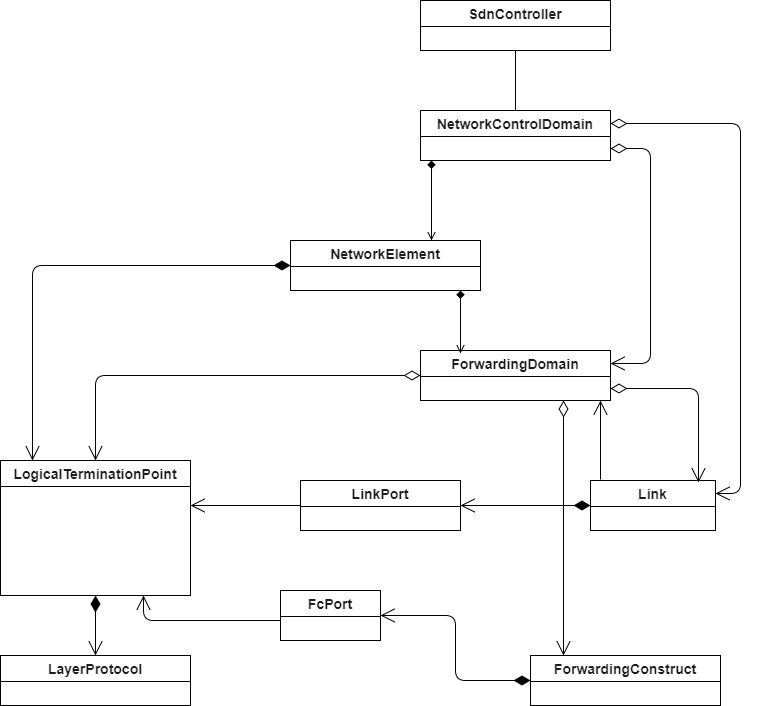
\includegraphics[width=1\textwidth]{core_model_uml_overview}
	\caption{Reprezentare UML simplificată a \textit{CoreModel}}
	\label{fig:core_model}
\end{figure}

O vedere de ansamblu simplificată, folosind \gls{uml} se poate vedea în Figura \ref{fig:core_model}. Blocurile relevante pentru simulatoarele dezvoltate vor fi detaliate în paragrafele următoare. Nu se vor detalia toate obiectele care alcătuiesc modelul informațional de bază deoarece, așa cum este sugerat în recomandarea \gls{onf}, modelul poate fi redus și simplificat, în funcție de nevoile pentru care este folosit.  

\subsection{Obiectul \textit{NetworkElement (NE)}}
%\paragraph{Network Element}

Obiectul \textit{NetworkElement} reprezintă un element de rețea - \gls{ne}, adică, în cazul \gls{sdn}, un echipament de dirijare din planul de date, sau, în cazul în care există virtualizare, un element virtual de rețea vizibil în interfaţa care folosește acea virtualizare.

Pentru o interfață directă între echipamentul de control \gls{sdn} către un echipament de rețea, obiectul \textit{NetworkElement} delimitează domeniul de control pentru resursele echipamentului, cum ar fi încapsularea folosită, multiplexarea, demultiplexarea, funcțiile asociate operaţiilor de administrare și de mentenanţă, etc. De asemenea, obiectul \textit{NetworkElement} defineşte domeniul spaţiilor de adresare pentru identificarea obiectelor care reprezintă resursele conţinute de echipamentul respectiv.

În cazul în care se folosesc metode de virtualizare, obiectul \textit{NetworkElement} reprezintă un element virtual de rețea. Asocierea unui element virtual cu unul real este responsabilitatea echipamentului de control \gls{sdn}. Cu ajutorul interfeţei de tip \textit{southbound} acesta poate crea sau şterge în mod dinamic astfel de obiecte pentru a oferi diferite vederi asupra rețelei, în funcție de nevoile aplicațiilor care se află deasupra echipamentului de control.

\subsection{Obiectele \textit{LogicalTerminationPoint (LTP)} și \textit{LayerProtocol (LP)}}

Obiectul \textit{LogicalTerminationPoint} - punct logic de terminaţie - cuprinde terminaţiile, adaptările sau funcțiile asociate operaţiilor de administrare și de mentenanţă ale unuia sau mai multor niveluri de transport. Prin natura sa, acest obiect suportă toate tipurile de protocoale, inclusiv cele pentru comutare de pachete sau pentru comutare de circuite. Fiecare nivel de transport este reprezentat de o instanţă a unui obiect \textit{LayerProtocol}, instanţă care poate fi folosită pentru a controla terminaţiile sau funcțiile de administrare și mentenanţă ale nivelului respectiv, sau pentru adaptarea (încapsularea sau multiplexarea semnalului client).

Dacă relația client-server între resursele echipamentului reprezentate de obiectele \textit{LTP} și \textit{LP} are un grad de asociativitate de 1:1 și este imuabilă, atunci un obiect \textit{LTP} poate conține mai multe obiecte \textit{LP}, de niveluri diferite de transport. Altfel, obiectele \textit{LP} de pe niveluri diferite trebuie să aibă asociate obiecte \textit{LTP} diferite.

Scopul acestor obiecte este acela de a oferi suport din perspectiva controlului și a administrării fără a fi nevoie de a defini atribute specifice unei anumite tehnologii, permițând astfel extinderea modelului fără a depinde de proprietățile tehnologiei respective, oferind flexibilitate sporită.

Un atribut important al obiectelor \textit{LP} este reprezentat de către \textit{layerProtocolName}. Acesta reprezintă nivelul de transport al obiectului și poate avea următoarele valori, conform \cite{onftr512v1.2}:

\begin{itemize}
	\item Nivel 0: \gls{ops}, \gls{ots}, \gls{oms}, \gls{och};
	\item Nivel 1: \gls{otu}, \gls{odu};
	\item Nivel 2: Carrier Ethernet: \gls{ety}, \gls{eth}; \gls{mpls-tp};
	\item Proprietăţi specifice nivelului de transport asociate cu obiectul \textit{LP}.
\end{itemize}

\subsection{Obiectul \textit{Forwarding Construct}}

Obiectele \textit{ForwardingConstruct (FC)} sunt folosite pentru a realiza dirijarea informației caracteristice nivelului de transport dat de obiectul \textit{LP} și oferă posibilitatea de a permite dirijarea între două sau mai multe obiecte \textit{LTP}. Astfel, obiectele \textit{FC} sunt independente de nivelul de transport folosit și suportă orice formă de pachete sau circuite.

Asocierea între \textit{FC} și \textit{LTP} se face prin port-uri, în care fiecare dintre acestea are un rol în contextul obiectului \textit{FC}. Dirijarea traficului între port-urile asociate se face în funcție de tipul de obiect \textit{FC}. Un astfel de obiect poate fi asociat unui singur obiect \textit{FD}. Ele pot fi definite recursiv (un obiect \textit{FC} poate fi parte din alt obiect \textit{FC}), însă la cel mai mic nivel de recursivitate acesta reprezintă de fapt o legătură în matricea de comutatoare a elementului de rețea.

Obiectele \textit{FC} pot fi folosite pentru a reprezenta orice fel de conexiune, cum ar fi punct la punct, punct la multi-punct sau multi-punct la multi-punct.

\subsection{Obiectul \textit{FC Port}}

Obiectele \textit{FC Port} sunt folosite, așa cum a fost prezentat anterior, la asocierea dintre obiectele \textit{FC} și \textit{LTP}. Dirijarea traficului între aceste obiecte se face conform tipului de \textit{FC}. De exemplu, \textit{FC Port} poate reprezenta un punct protejat (de încredere) sau un punct care protejează (de rezervă), în cazul în care rolul obiectului \textit{FC} este unul de protecție.

\subsection{Obiectul \textit{Forwarding Domain}}

\textit{ForwardingDomain} - domeniul de dirijare - este un obiect care modelează componenta topologiei care permite dirijarea pachetelor între diferite puncte ale resurselor echipamentului de rețea (reprezentate prin alte obiecte, de tipul \textit{LogicalTerminationPoint}). Lista punctelor logice de terminaţie care pot fi folosite de către un domeniu de dirijare este parte a acestui obiect. \textit{ForwardingDomain} poate conţine zero sau mai multe obiecte de tip \textit{ForwardingConstruct}, indiferent de nivelul la care se află acestea (Ethernet, MPLS, optic, etc.). 

Acest domeniu de dirijare oferă contextul pentru crearea, modificarea sau ștergerea obiectelor de tip \textit{ForwardingConstruct}. Obiectul \textit{ForwardingDomain} dintr-un element de rețea poate reprezenta comutatorul sau gruparea de comutatoare din echipamentul de dirijare.


\section{ONF TR-532 - Modelul informaţional pentru microunde (\textit{Microwave Information Model})}

Modelul informațional pentru microunde \cite{onftr532} a apărut in decembrie 2016 ca o recomandare formulată de grupul \gls{otwg} din cadrul \gls{onf}. Scopul acestuia este de a modela un echipament de transport de date fără fir, pentru a putea fi folosit de echipamentele de control \gls{sdn}, în încercarea de a asigura o independenţă față de producătorii de echipamente. Chiar dacă este denumit \textit{model informațional pentru microunde}, acesta poate fi aplicat fără probleme nu numai echipamentelor ce funcționează în spectrul microundelor, ci și echipamentelor care funcționează în benzi de frecvenţă mai înalte (lungimi de undă milimetrice), care încep să își facă tot mai mult simţită prezenţa în rețelele actuale de transport.

TR-532 este de fapt o extensie specifică tehnologiei \gls{wt} a modelului informațional de bază, versiunea 1.2 (TR-512.1). Legătura cu acesta se face prin extinderea clasei de obiecte \textit{\gls{lp}}. Astfel, modelul informațional pentru microunde conţine şase pachete condiţionale caracteristice tehnologiilor folosite pentru transport, care au în nume extensia \textit{*\_Pac}: 

\begin{itemize}
	\item \textit{MW\_AirInterface\_Pac};
	\item \textit{MW\_AirInterfaceDiversity\_Pac};
	\item \textit{MW\_PureEthernetStructure\_Pac};
	\item \textit{MW\_HybridMWStructure\_Pac};
	\item \textit{MW\_EthernetContainer\_Pac};
	\item \textit{MW\_TdmContainer\_Pac}
\end{itemize}

O imagine de ansamblu simplificată a acestui model, în limbajul \gls{uml}, care conţine doar obiectele relevante pentru simulatoarele dezvoltate, împreună cu legătura acestuia cu modelul informațional de bază este ilustrată în Figura \ref{fig:microwave_model}.

\begin{figure}[h]
	\centering
	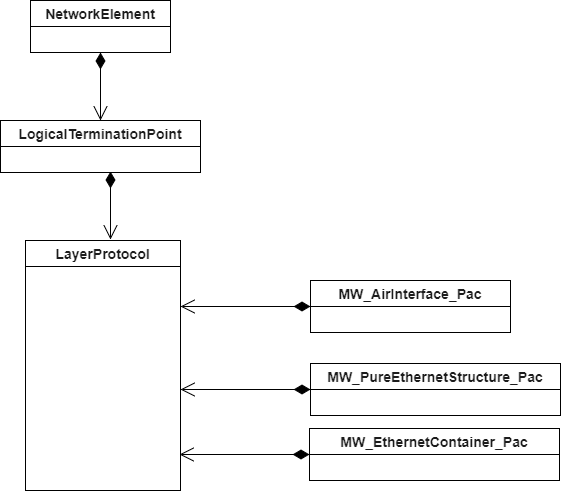
\includegraphics[width=1\textwidth]{microwave_model_overview}
	\caption{Reprezentare UML simplificată a \textit{MicrowaveModel} și legătura acestuia cu \textit{CoreModel} \cite{onftr532}.}
	\label{fig:microwave_model}
\end{figure}

În următoarele paragrafe se vor detalia obiectele acestui model care sunt importante din punctul de vedere al simulatoarelor dezvoltate în această lucrare.

\subsection{Obiectul \textit{MW\_AirInterface\_Pac}}

Obiectul \textit{MW\_AirInterface\_Pac} reprezintă o interfață radio fizică a unui echipament. Este denumit în recomandare ca \textit{punct de terminaţie a traseului secţiunii fizice de microunde} - \gls{mwps-ttp}, astfel că nivelul de transport al obiectului \textit{\gls{lp}} asociat este Secţiunea Fizică de Microunde - \textit{\gls{mwps}} \cite{onftr532}. O reprezentare simplificată în limbajul \gls{uml} a \textit{MW\_AirInterface\_Pac} se poate observa în Figura \ref{fig:airinterface_pac}.

\begin{figure}[h]
	\centering
	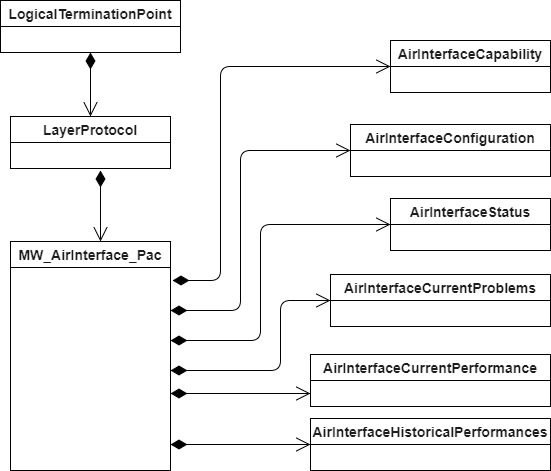
\includegraphics[width=1\textwidth]{airinterface_pac}
	\caption{Reprezentare UML simplificată a obiectului \textit{MW\_AirInterface\_Pac} \cite{onftr532}.}
	\label{fig:airinterface_pac}
\end{figure}

Acest obiect conţine alte câteva obiecte care modelează caracteristice unei interfețe radio fizice, cum ar fi: (i) capabilităţi ale modemului și ale transmiţătorului interfeţei radio asociate (de exemplu tipurile de modulaţie suportate pentru transmisie, valorile admisibile ale puterii de transmisie, intervalul de frecvenţe suportate de emiţător sau de receptor, alarmele expuse de interfață, suportul interfeţei pentru modulaţie adaptivă, etc.), (ii) parametrii configurabili ai interfeţei radio (de exemplu numele interfeţei, lărgimea de bandă a canalului de transmisie/de recepţie, frecvenţele folosite pentru transmisie/recepţie, puterea de transmisie, intervalul în care modulaţia poate lua valori, diferite alte caracteristici configurabile ale interfeţei, cum ar fi Anularea Interferenţei dintre Polarizări - \gls{xpic}, Intrări Multiple - Ieşiri multiple - \gls{mimo}, criptarea datelor, etc.), (iii) parametrii care descriu starea interfeţei la un anumit moment de timp (de exemplu frecvenţele actuale de transmisie/recepţie, nivelurile actuale de putere a semnalului de transmisie/recepţie, modulaţia actuală folosită, raportul semnal-zgomot măsurat de către modem, temperatura actuală a unităţii radio, etc.), (iv) problemele actuale ale interfeţei radio (adică alarmele care apar pe interfață la un moment dat), (v) valorile actuale ale parametrilor de performanţă a interfeţei și (vi) valorile istorice ale parametrilor de performanţă a interfeţei \cite{onftr532}.

\subsection{Obiectul \textit{MW\_PureEthernetStructure\_Pac}}

Obiectul \textit{MW\_PureEthernetStructure\_Pac} este o reprezentare logică a unei interfețe radio capabilă să transporte doar trafic Ethernet. Acest obiect este reprezentat într-un mod simplificat, în limbajul \gls{uml}, în Figura \ref{fig:pureethstructure_pac}. Asocierea cu o interfață fizică radio se face la nivelul modelului informațional de bază, printr-o relaţie de tip client-server.

\begin{figure}[h]
	\centering
	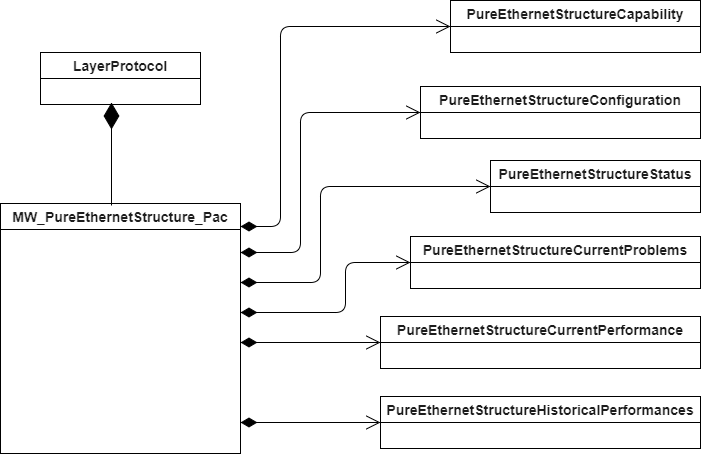
\includegraphics[width=1\textwidth]{pureethstructure_pac}
	\caption{Reprezentare UML simplificată a obiectului \textit{MW\_PureEthernetStructure\_Pac} \cite{onftr532}.}
	\label{fig:pureethstructure_pac}
\end{figure}

Acest obiect este denumit în recomandare ca \textit{punct de terminaţie a traseului secţiunii microunde} - \gls{mws-ttp}, astfel că nivelul de transport al obiectului \textit{\gls{lp}} asociat este Secținea de Microunde - \textit{\gls{mws}}. 

Structura obiectelor conţinute de către \textit{MW\_PureEthernetStructure\_Pac} este similară cu cea a obiectului \textit{MW\_AirInterface\_Pac}. Conţine obiecte care reprezintă (i) capabilitățile acestei interfețe logice (de exemplu alarmele aplicabile ei sau identificatorul structurii respective, care poate fi folosit de alte obiecte), (ii) parametrii configurabili ai interfeţei logice (de exemplu gradul de severitate a alarmelor pe care această interfață le expune), (iii) parametrii care descriu starea interfeţei logice la un anumit moment de timp, (iv) problemele actuale ale interfeţei logice, (v) valorile actuale ale parametrilor de performanţă a interfeţei logice și (vi) valorile istorice ale parametrilor de performanţă a interfeţei logice \cite{onftr532}.

\subsection{Obiectul \textit{MW\_EthernetContainer\_Pac}}

Obiectul \textit{MW\_EthernetContainer\_Pac} reprezintă de asemenea o interfață logică și este denumit în recomandare \textit{punct de terminaţie a conexiunii unui client de microunde}, pentru un semnal Ethernet client. Practic, este o interfață logică ce are rol de container pentru traficul Ethernet care este transmis de echipament prin radio. În raport cu obiectul \textit{\gls{lp}} acesta are un nivel de transport denumit Container Ethernet - \textit{\gls{etc}}. O reprezentare grafică simplificată în limbajul \gls{uml} a obiectului \textit{MW\_EthernetContainer\_Pac} poate fi găsită în Figura \ref{fig:ethcontainer_pac}.

\begin{figure}[h]
	\centering
	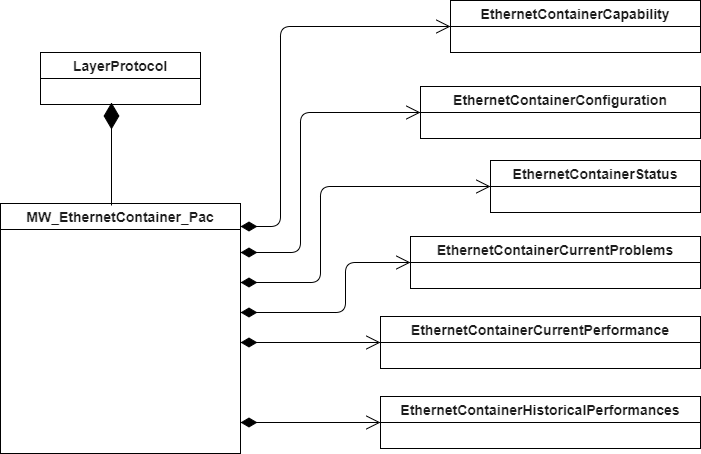
\includegraphics[width=1\textwidth]{ethcontainer_pac}
	\caption{Reprezentare UML simplificată a obiectului \textit{MW\_EthernetContainer\_Pac} \cite{onftr532}.}
	\label{fig:ethcontainer_pac}
\end{figure}

Și în cazul obiectului \textit{MW\_EthernetContainer\_Pac} se păstrează aceeaşi structura a obiectelor pe care le conţine, ca în cazul celorlalte două obiecte detaliate anterior. Astfel, acesta prezintă obiecte care reprezintă (i) capabilitățile containerului (de exemplu dacă există compresie la diferite niveluri, criptare a datelor sau alarmele pe care această interfață le expune), (ii) parametrii configurabili ai containerului (de exemplu un identificator al containerului, identificatoarele segmentelor folosite pentru a transporta traficul Ethernet asociat acestui container, etc.), (iii) parametrii care descriu starea containerului, (iv) alarmele la momentul actual de timp pe care containerul le raportează, (v) valorile actuale ale parametrilor de performanţă a containerului și (vi) valorile istorice ale parametrilor de performanţă a containerului \cite{onftr532}.
\section{Protocolul NETCONF}

Standardizare: ONF, etc..
\section{Alegerea unei soluții software pentru serverul NETCONF}

Există numeroase soluții care lucrează cu protocolul \gls{netconf}, atât pe partea de client, cât și pe cea de server. O listă a acestora este menţinută de către grupul de lucru \gls{netconf} și poate fi găsită online \cite{netconfwiki}. Conţine și soluții software proprietare, dar și soluții cu sursă deschisă. Pentru implementarea simulatoarelor prezentate în această lucrare au fost considerate trei opţiuni de implementare a unui server \gls{netconf}, cu sursă deschisă: \textit{Netopeer}, \textit{OpenYuma} și \textit{\gls{netconf} Test Tool} (unealtă oferită de proiectul \gls{odl}). O comparaţie între acestea va fi prezentată în continuare, justificând astfel alegerea de a folosi una dintre ele în simulatoare \cite{stancu2016comparison}.

\subsection{Netopeer}

\textit{Netopeer} este o soluție ce se bazează pe librăria \textit{libnetconf}, oferind atât o implementare pentru server, cât și una pentru un client al serverului. Această librărie este una cu sursă deschisă, implementată în limbajul C, ce oferă o implementare a protocolului \gls{netconf} \cite{krejci2013building}. Este o soluție care poate fi personalizată, oferind numeroase posibilităţi pentru implementările de server și de client și suportă toate caracteristicile protocolului \gls{netconf}.

\textit{Netopeer} oferă câteva unelte, de exemplu pentru a facilita integrarea modelelor informaționale \gls{yang} în module ale serverului, denumită \textit{administrator-netopeer - netopeer-manager}, sau pentru a configura caracteristicile serverului \gls{netconf}. Orice model de date \gls{yang} poate fi adăugat ca un modul al serverului, însă acesta trebuie prelucrat înainte. Astfel, fişierul \textit{*.yang} este transformat de către această soluție în fişiere pe care serverul le poate recunoaşte, inclusiv un fişier \textit{*.c}, care conţine un schelet de cod C, reprezentând așa-numite funcții cu apel invers (\textit{callback functions}) ce pot fi implementate pentru ca serverul să ofere comportamentul dorit, în raport cu modelul \gls{yang} folosit. Apoi, codul C este compilat, rezultând o bibliotecă partajată (\textit{shared library}) care poate fi utilizată de către codul de bază al serverului.

\subsection{OpenYuma}

\textit{OpenYuma} este o soluție software care se bazează pe proiectul \textit{Yuma}, care a devenit proprietar în anul 2011. Propune de asemenea implementări pentru server și client \gls{netconf}, scrise în limbajul C, oferind chiar posibilitatea de a încorpora acest cod în dispozitive al căror software folosește tot limbajul C.

\textit{OpenYuma} are o filosofie asemănătoare cu \textit{Netopeer}, oferind unelte pentru transformarea modelelor \gls{yang} în cod C schelet, care să fie apoi implementat pentru ca serverul \gls{netconf} să ofere facilităţile propuse. Unealta propusă de această soluție software se numeşte \textit{yangudmp} și transformă fişierele \textit{*.yang} în fişiere \textit{*.h} și \textit{*.c}, conţinând, la fel ca în cazul \textit{Netopeer}, funcții de apel invers ce trebuie rescrise.

Codul C obţinut după transformarea modelelor \gls{yang} se compilează, rezultând tot o bibliotecă partajată care să poată fi folosită de către codul de cază al serverului. Aceasta poate fi încărcată în momentul inițializării serverului sau chiar în mod dinamic, în timp ce acesta rulează.

\subsection{Unealta de Test Netconf - \textit{Netconf Testtool}}

Unealta de Test Netconf este o soluție software oferită în cadrul proiectului OpenDaylight \cite{odlnetconftesttool}. Este o soluție simplă, care nu poate fi personalizată foarte mult, oferind doar o implementare Java pentru un server \gls{netconf}. Aceasta este folosită de proiectul \gls{odl} pentru a-și testa interfaţa de Sud care implementează protocolul \gls{netconf}.

Scopul acestei soluții este puţin diferit de al celorlalte, deoarece \textit{Testtool} nu își propune oferirea unei soluții software care implementează un server \gls{netconf} care apoi să poată fi integrat cu echipamentele de rețea, ci oferirea unei soluții simple și rapide care să încarce un model \gls{yang} specific, cu scopul de a-l testa. Cu toate acestea, acest software a fost considerat pentru comparaţie, deoarece și scopul simulatoarelor este de a testa modelele \gls{yang} și de a crea topologii specifice rețelelor de transport de date fără fir, expunând modelele informaționale descrise anterior.

\subsection{Comparaţie între soluţiile care oferă server NETCONF}

Soluţiile descrise anterior au fost evaluate atât prin compararea documentaţiei relevante pe care acestea o pun la dispoziţie, cât și prin experimente practice care iar în considerare diferite scenarii. 

Comparaţia bazată pe lucrurile descrise în documentaţie este rezumată în Tabelul \ref{tab:Table_1}, în timp ce un sumar al comparaţiei bazată pe experimentare se găseşte în Tabelul \ref{tab:Table_2}.

\begin{table}[hp]
	\caption{Comparaţie a caracteristicilor oferite de cadrele software considerate.\label{tab:Table_1}}
	
	\begin{tabular}{|M{0.35\textwidth}|M{0.17\textwidth}|M{0.17\textwidth}|M{0.16\textwidth}|}
		\hline 
		\textbf{Criteriile} & \multicolumn{3}{c|}{\textbf{Soluții servere NETCONF}} \tabularnewline
		\cline{2-4} 
		\textbf{de comparație} & \textbf{\emph{Netopeer}} & \textbf{\emph{OpenYuma}} & \textbf{\emph{Testtool}}\tabularnewline
		\hline 
		Limbajul de programare & C & C & Java\tabularnewline
		\hline 
		Încărcarea modelelor YANG brute & Nu & Nu & Da\tabularnewline
		\hline 
		Încărcarea dinamică a modulelor în server & Da & Da & Nu\tabularnewline
		\hline 
		Baza de stocare a datelor NETCONF & toate & toate & de operare \tabularnewline
		\hline 
		Suport pentru notificări & da & da & da\tabularnewline
		\hline 
		Port configurabil & da & da & da\tabularnewline
		\hline 
		Mai multe instanțe de server & nu & da & da \tabularnewline
		\hline 
		Mai multe conexiuni în același timp & da & da & da\tabularnewline
		\hline 
		Capabilități pentru depanare & jurnalizare & jurnalizare & jurnalizare\tabularnewline
		\hline
	\end{tabular}
\end{table}

Primul criteriu care poate fi considerat este limbajul pe programare în care aceste soluții software sunt implementate: \textit{Netopeer} și \textit{OpenYuma} sunt scrise în limbajul C, pe când \textit{Testtool} este o implementare Java.

Un alt criteriu pentru evaluare constă în abilitatea serverului de a încărca în mod direct (dinamic sau în momentul inițializării) modele \gls{yang}. Această posibilitate este oferită doar de implementarea Java. Celelalte două soluții au nevoie de o fază premergătoare de procesare,transformând fişierele \textit{*.yang} în \textit{*.c}. \textit{Netconf Test Tool} poate încărca modelul \gls{yang} doar în momentul inițializării serverului, dintr-un director anume, pe când celelalte cadre software pot încărca acest model, după ce a fost procesat, în mod dinamic.

Un alt subiect pentru comparaţie este dat de tipurile de baze de stocare de date propuse de protocolul \gls{netconf} suportate de implementările serverelor. \textit{Netopeer} și \textit{OpenYuma} folosesc fişiere \gls{xml} în care stochează informaţiile și suportă toate cele trei tipuri de baze de stocare a datelor propuse de \gls{netconf}: de iniţializare, de rezervă și de operare. Cealaltă soluție software, \textit{Testtool} oferă posibilitatea de a utiliza doar baza de stocare de date de operare stocând valorile parametrilor în variabile de execuţie, acestea pierzându-se în momentul în care serverul este oprit. O diferenţă importantă apare în acest context, între cele două soluții implementate în C, \textit{OpenYuma} oferind o flexibilitate mai mare. În cazul \textit{Netopeer}, atunci când serverul se iniţializează, încarcă valorile parametrilor din bazele de stocare de date de iniţializare și de operare în memorie. Apoi, începe să analizeze valorile din baza de stocare de date de iniţializare, comparându-le cu valorile corespunzătoare atributelor din cea de operare. Dacă valorile nu sunt egale, sau valoarea din baza de stocare de date de operare nu există (însemnând prima utilizare a serverului), atunci serverul copiază valoarea din baza de stocare de date de iniţializare și apelează funcţia de apel invers asociată parametrului de configurare. Prin această abordare severul se asigură ca nu există inconsistenţe între bazele de stocare de date de iniţializare și de operare și, mai mult, dacă acest server este conectat la un echipament real de rețea, prin apelarea funcţiei cu apel invers asociate parametrului, dispozitivul va fi configurat astfel încât valorile din server să reflecte valorile de pe echipament. \textit{OpenYuma} are o abordare mai flexibilă, permiţând dezvoltatorilor să altereze baza de stocare de date de operare în timpul inițializării modulului, fără a implica baza de stocare de date de iniţializare.

\begin{table}[tp]
	
	\caption{Compararea practică a cadrelor software considerate\label{tab:Table_2}}
	\begin{tabular}{|M{0.35\textwidth}|M{0.17\textwidth}|M{0.17\textwidth}|M{0.16\textwidth}|}
		\hline
		\textbf{Scenariul experimentat} & \textbf{\emph{Netopeer}} & \textbf{\emph{OpenYuma}} & \textbf{\emph{Testtool}} \tabularnewline
		\hline 
		Procesarea \textit{*.yang} în \textit{*.c} & lnctool & yangdump & N/A\tabularnewline
		\hline 
		Reprezentarea bazei de stocare a datelor în cadrul serverului & fişier XML & fișier XML & variabile de execuție \tabularnewline
		\hline 
		Încărcarea datelor în faza de iniţializare a serverului & \textit{startup} & flexibilă, orice se poate suprascrie & N/A \tabularnewline
		\hline 
		Implementarea notificărilor NETCONF & \textit{libnetconf} & funcție cu apel invers oferită & fișier XML \tabularnewline
		\hline 
		Funcții pentru parametrii configurabili & câte una per atribut & câte una per atribut & N/A\tabularnewline
		\hline 
		Funcții pentru parametrii de stare & doar una, globală & câte una per atribut & N/A\tabularnewline
		\hline 
		Conexiuni concurente de la clienți & da & suportă, trebuie implementat & da\tabularnewline
		\hline \end{tabular}
\end{table}

O altă caracteristică importantă a serverelor care poate fi comparată este abilitatea de a genera notificări \gls{netconf}. Toate cele trei soluții oferă notificări. În cazul \textit{Testtool} este o implementare simplă, acestea fiind declanşate printr-o comandă \gls{netconf} și trimise dintr-un fişier \gls{xml} care le conţine. \textit{OpenYuma} oferă câte o funcție cu apel invers pentru fiecare notificare pe care o găseşte în momentul procesării modelului \gls{yang}. \textit{Netopeer} nu are această abilitate în mod implicit, însă suportul este oferit de \textit{libnetconf}.

Din perspectiva funcţiilor cu apel invers generate în momentul procesării modelului \gls{yang} putem compara doar cele două soluții implementate în limbajul C, deoarece \textit{Testtool} nu oferă astfel de caracteristici. Soluția \textit{Netopeer} oferă posibilitatea de a alege care dintre parametrii configurabili vor avea o funcție cu apel invers asociată, în timp ce \textit{OpenYuma} va genera o astfel de funcție pentru fiecare din parametrii configurabili pe care îi găseşte în modelul \gls{yang}. Pentru informaţiile de stare \textit{Netopeer} generează o singură funcție cu apel invers care este apelată pentru orice operaţie \gls{netconf} de tip \textit{get} care ajunge la server, iar \textit{OpenYuma} generează câte o astfel de funcție pentru fiecare parametru de stare.

Din punctul de vedere al abilităţii de a configura portul pe care serverul acceptă conexiuni, toate soluţiile oferă această posibilitate. \textit{Testtool} are nevoie de un port de plecare, incrementând apoi numărul portului pentru celelalte instanţe ale serverului. Și celelalte soluții oferă posibilitatea de a schimba portul pe care serverul ascultă. Din perspectiva rulării mai multor instanţe de server pe aceeaşi mașină, atât \textit{Testtool} cât și \textit{OpenYuma} oferă această posibilitate, diferitele instanţe folosind porturi diferite. \textit{Netopeer}, pe de altă parte, nu permite rularea mai multor instanţe pe aceeaşi mașină.

Un alt criteriu pentru compararea acestor cadre software este dat de suportul pentru mai multe fire de execuție, adică abilitatea serverului de a permite conectarea mai multor clienţi în același timp. \textit{Testtool} oferă această posibilitate. \textit{OpenYuma} oferă de asemenea acest suport, cu menţiunea că accesul concurent la resursele comune trebuie rezolvat în funcțiile cu apel invers care vor fi implementate de către dezvoltatori, nefiind rezolvat de către cadrul software. În cazul \textit{Netopeer}, acest acces concurent este rezolvat din faza de proiectare a serverului și este oferit de \textit{libnetconf}.

Și capabilitățile de depanare oferite ar putea constitui un criteriu de comparaţie, însă toate soluţiile se bazează pe fişiere de tip jurnal, oferind mai multe niveluri de jurnalizare.

Pe baza acestei comparaţii a fost aleasă soluţia \textit{OpenYuma} pentru implementarea serverului \gls{netconf} folosit în simulatoare, ea oferind cea mai mare flexibilitate.
\section{Arhitectura demonstraţiilor de concept WT SDN}

Standardizare: ONF, etc..

\chapter{Mediatorul cu valori implicite (DVM)\label{ch:dvm_v01}}

\graphicspath{ {cap-dvm_v01/figures/} }

Nivelul mediator a apărut în arhitectura demonstraţiilor de concept, cum a fost prezentat anterior, deoarece dispozitivele de rețea încă nu au suport pentru modelul informațional pentru microunde TR-532. Astfel, această aplicație software trebuie să traducă operaţiile \gls{netconf} care vin de la echipamentul de control într-un limbaj care să fie recunoscut de echipamente. Fiecare producător de dispozitive care a participat la cea de-a doua demonstraţie de concept \gls{wt} \gls{sdn} a fost nevoit să implementeze un astfel de mediator.

Am dezvoltat mediatorul cu valori implicite (\textit{Default Values Mediator - \gls{dvm}}) special pentru cea de-a doua demonstrație de concept \gls{wt} a \gls{onf}, pentru a oferi posibilitatea dezvoltatorilor de aplicații \gls{sdn} care nu au acces la echipament de transport de date fără fir și la mediatoarele asociate acestora posibilitatea de a implementa și testa astfel de aplicații, care vor putea apoi interacţiona cu mediatoare reale, pentru că folosesc aceeaşi interfață \gls{netconf} care expune modelul informațional de bază și modelul informațional pentru microunde. Apoi, această implementare a evoluat în cea de-a doua versiune a \gls{dvm}, care a fost folosită pentru ce-a de-a doua demonstrație de concept.

\gls{dvm} este o implementare software cu sursă deschisă a unui server \gls{netconf}, bazându-se pe soluţia software \textit{OpenYuma}. Spre deosebire de mediatoarele reale, \textit{\gls{dvm}} are o singură interfață (cea prin care comunică cu controlerul \gls{sdn}), neavând nevoie de o interfață care să se lege la dispozitive reale de rețea. Acest simulator va returna valori implicite pentru atributele interogate de către controler.

\section{Arhitectura}

SDN și reţelele actuale..
\section{Implementarea DVM versiunea 1}

Primul pas al implementării a fost reprezentat de alegerea modelelor \gls{yang} care să fie expuse de serverul \gls{netconf}. În cea de-a doua demonstraţie de concept \gls{wt} a fost agreată folosirea unor modele informaționale reduse, care să permită demonstrarea cazurilor de utilizare alese \cite{onf2016_poc2}. Acestea conţineau aproximativ şaizeci de atribute care făceau parte atât din modelul informațional de bază, cât și din modelul informațional pentru microunde. Astfel, au fost alese trei modele \gls{yang} pentru implementarea în cadrul primei versiuni a \gls{dvm}: \textit{CoreModel-CoreNetworkModule-ObjectClasses}, \textit{MicrowaveModel-ObjectClasses-MwConnection} și \textit{MicrowaveModel-Notifications}. Asta a însemnat, practic, generarea a trei biblioteci partajate reprezentând module ale serverului \gls{netconf}, care să poată fi încărcate în soluţia \textit{OpenYuma} și să ofere capabilitățile dorite.

O organigramă a fazei de dezvoltare și implementare a \gls{dvm} este ilustrată în Figura \ref{fig:dvm_v01_workflow}.

\begin{figure}[h]
	\centering
	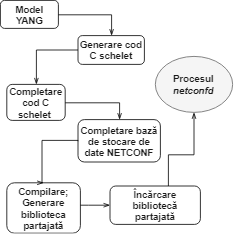
\includegraphics{dvm_v01_workflow}
	\caption{Organigramă a dezvoltării și implementării DVM \cite{stancu2016default}.}
	\label{fig:dvm_v01_workflow}
\end{figure}

Cel de-al doilea pas al implementării a constat în procesarea modelelor \gls{yang} alese și generarea codului C schelet al modulelor asociate acestora. Acest lucru a fost realizat cu utilitarul \textit{yangdump} oferit de soluţia \textit{OpenYuma}. Pentru a îmbunătăţi flexibilitatea \gls{dvm} și pentru a avea o mai bună separare între codul folosit de server și codul utilizatorului, care trebuie rescris, utilitarul a fost folosit cu opţiunea \textit{--split}. Astfel, pentru fiecare modul au fost generate patru fişiere: câte unul \textit{.c} și \textit{.h} pentru codul de server, respectiv pentru cel de utilizator.

Următorul pas a fost reprezentat de implementarea funcţiilor cu apel invers generate pentru fiecare atribut al modelului \gls{yang}. Pentru a asocia câte o valoare implicită fiecărui parametru, funcțiile au fost modificate astfel încât să întoarcă valoarea respectivă în momentul apelării.

Cea mai importantă parte a implementării \gls{dvm} a constat în construirea bazei de stocare a datelor de operare, reprezentând de fapt arborele atributelor \gls{yang} pe care serverul \gls{netconf} le va utiliza atunci când va fi interogat de către echipamentul de control \gls{sdn}. Nu a fost posibilă construirea automată a acestui arbore de parametri, astfel că atributele au fost implementate manual, de la rădăcină către frunze. Pentru acest lucru a fost nevoie să se altereze funcţia de iniţializare \textit{init2()} generată automat pentru fiecare model \gls{yang}. A fost necesară adăugarea câte unui nod \textit{OpenYuma} pentru fiecare parametru \gls{yang}, având asociată o funcție cu apel invers în care se setează valoarea implicită a acelui atribut. În cazul parametrilor anterior menţionaţi, care fac parte din fişierul de configurare, implementarea funcţiei constă în citirea valorii respective din acel fişier. Această abordare a permis utilizatorilor \gls{dvm} un acces facil la valorile implicite asociate fiecărui atribut. Dacă un utilizator avea nevoie de schimbarea valorii unui parametru \gls{yang}, o putea face uşor prin funcţia cu apel invers asociată sau prin fişierul de configurare, fără să fie nevoit să ştie detaliile de implementare referitoare la construirea arborelui de valori.

Următorii paşi ai implementării sunt simpli și direcţi: codul rezultat se compilează, rezultând bibliotecile partajate care apoi sunt încărcate în serverul \gls{netconf} (mai exact în procesul \textit{netconfd} asociat acestuia).

Etapele anterior menţionate se aplică în cazul modelului informațional de bază și în cazul modelului informațional pentru microunde, excluzând cazul notificărilor \gls{netconf}, unde abordarea este puţin diferită.

Deoarece modelul asociat notificărilor \gls{netconf}, \textit{MicrowaveModel-Notifications}, are o structură diferită, conţinând obiecte \gls{yang} ce reprezintă notificări în locul atributelor obişnuite, comportamentul soluţiei \textit{OpenYuma} este diferit în acest caz. În loc să se genereze funcții cu apel invers pentru obţinerea și setarea valorilor atributelor, în cazul notificărilor soluţia \textit{OpenYuma} va genera funcții cu apel invers folosite pentru declanşarea acestora (trimiterea lor de către server tuturor utilizatorilor care s-au abonat).

Pentru implementarea notificărilor \gls{netconf} în \gls{dvm}, un nou fir de execuţie s-a creat în funcţia de iniţializare a modulului, \textit{init2()}. Acesta rulează o singură funcție care implementează o buclă infinită în care se folosește funcţia cu apel invers asociată pentru a trimite o notificare fictivă, la un interval de secunde definit în fişierul de configurare. În cazul în care valoarea intervalului este zero, declanşarea notificărilor nu va fi activată. Detaliile conţinute în notificarea \gls{netconf} fictivă se găsesc în interiorul funcţiei care implementează generarea și modificarea acestora nu este banală pentru un utilizator neexperimentat.

Structura fişierului de configurare este foarte simplă și nu oferă prea multă flexibilitate utilizatorilor \gls{dvm}. Aceasta este fixă și poate fi observată în Figura \ref{fig:dvm_v01_config}, într-un exemplu în care un dispozitiv conţine două interfețe radio. Conţine doar trei tipuri de parametri, așa cum a fost menţionat anterior: numele echipamentului de rețea (\textit{NeName}), identificatoarele legăturilor radio (\textit{radioSignalId} - există câte un identificator pentru fiecare interfață radio a dispozitivului) și intervalul de timp, exprimat în secunde, dintre două notificări fictive consecutive (\textit{eventFrequency}).

\begin{figure}[h]
	\centering
	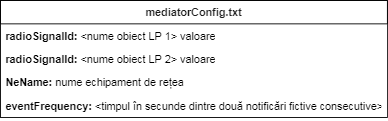
\includegraphics{dvm_v01_config}
	\caption{Structura fişierului de configurare al DVM. Exemplu pentru un echipament cu două interfețe radio.}
	\label{fig:dvm_v01_config}
\end{figure}
\section{Folosirea în contextul demonstraţiilor de concept a DVM versiunea 1}

Prima versiune a mediatorului cu valori implicite a fost o unealtă foarte importantă în contextul celei de-a doua demonstraţii de concept a proiectului rețelelor de transport de date fără fir din cadrul \gls{onf}. Acesta a ajutat la accelerarea implementării aplicațiilor \gls{sdn} care au fost dezvoltate pentru cazurile de utilizare propuse în \cite{onf2016_poc2}.

\gls{dvm} a oferit interfaţa de Sud \gls{netconf} care expune modelele informaționale dezvoltate de \gls{onf}, în același mod în care ar expune-o un mediator real ce se conectează la echipamente de transport de date fără fir. În acest mod, dezvoltatorii aplicațiilor \gls{sdn} au putut utiliza acest simulator pentru implementarea și testarea acestora, fără a avea nevoie să deţină dispozitive de rețea, care au un preţ foarte ridicat.

Această primă versiune de simulator a accelerat activitățile de pregătire a celei de-a doua demonstraţii de concept, permiţând lucrul în paralel la aplicațiile \gls{sdn} și la dezvoltarea mediatoarelor. Interfaţa \gls{netconf} comună a putut fi testată înainte ca producătorii de echipamente să își implementeze mediatoarele, oferind astfel mai mult timp dezvoltatorilor aplicațiilor \gls{sdn} pentru depanarea programelor. De exemplu, generarea unei notificări \gls{netconf} se poate face mult mai facil cu ajutorul simulatorului. Pentru un mediator real, trebuie ca dispozitivul să fie făcut să genereze o notificare către mediator, prin interfaţa proprietară echipamentului respectiv, apoi mediatorul să traducă acel mesaj într-o notificare \gls{netconf}.

Figura \ref{fig:dvmv01_poc_usage} reprezintă elementele de bază ale demonstraţiei de concept, așa cum sunt prezentate în lucrarea apărută după desfăşurarea acestuia \cite{onf2016_poc2}, în care se poate vedea \gls{dvm}.

\begin{figure}[h]
	\centering
	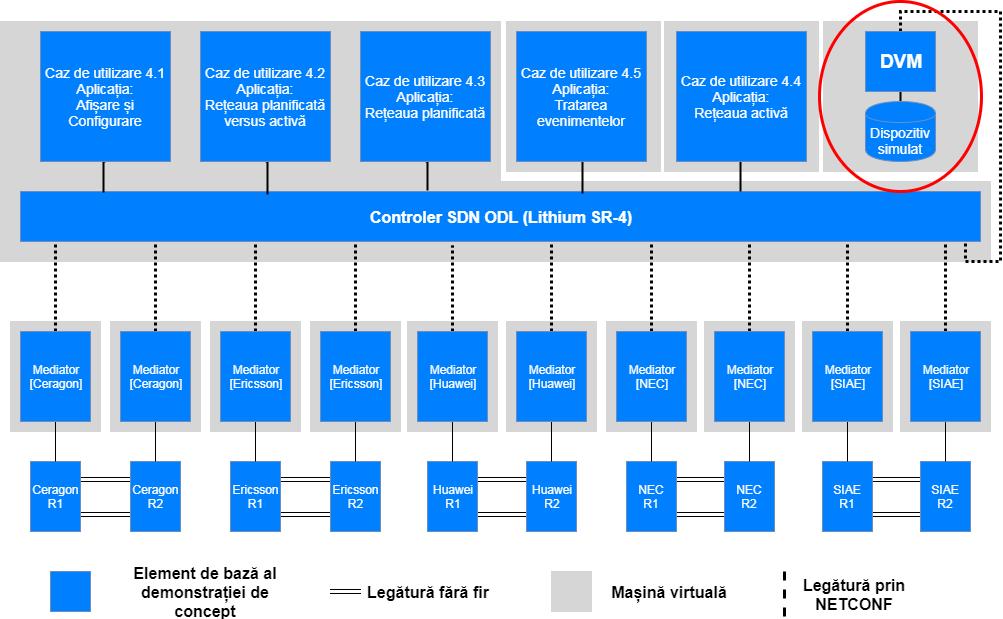
\includegraphics[width=1\textwidth]{dvmv01_poc_usage}
	\caption{Configurarea rețelei de test SDN utilizând mașini virtuale \cite{onf2016_poc2}.}
	\label{fig:dvmv01_poc_usage}
\end{figure}

Înregistrarea la controlerul \gls{sdn} a primei versiuni a simulatoarelor \gls{dvm}, se face la fel ca pentru un mediator real. Astfel, echipamentul de control oferă o interfață de programare a aplicaţiei - \gls{api} - prin care o aplicație \gls{sdn} poate înregistra un astfel de mediator în controlerul \gls{sdn}. Înregistrarea nu este una automată, utilizatorul fiind nevoit să facă această înregistrare manual. În cea de-a doua demonstraţie de concept, acest lucru a fost făcut prin interfaţa grafică a echipamentului de control folosit (\gls{odl}). După înregistrare, controlerul stabileşte conexiunea \gls{netconf} cu mediatorul.

Codul asociat primei versiuni a \gls{dvm} este oferit cu sursă deschisă și se poate găsi în repertoriul asociat \gls{onf} de pe platforma GitHub, denumit CENTENNIAL \cite{dvmv01github}.
\section{Arhitectura DVM versiunea 2}

Cea de-a doua versiune a \gls{dvm} a fost implementată pentru a treia demonstraţie de concept a rețelelor de transport de date fără fir desfăşurată în cadrul \gls{onf}. A fost dezvoltată pe scheletul primei versiuni, păstrând aceeaşi abordare: un server \gls{netconf} care se bazează pe soluţia software \textit{OpenYuma} și un fişier de configurare din care serverul poate citi valori pentru atributele \gls{yang} pe care le expune. Din acest punct de vedere, \gls{dvm} versiunea 2 folosește întregul model informațional pentru microunde TR-532 și o parte semnificativă din modelul informațional de bază, TR-512.1, cumulând aproximativ 300 de astfel de parametri.

Arhitectura celei de-a doua versiuni a \gls{dvm} este influenţată de natura atributelor \gls{yang} ce alcătuiesc modelul informațional pentru microunde \cite{stancu2017enabling}: parametri de configurare, de stare sau care prezintă capabilitățile dispozitivului. Atributele de configurare pot fi citite sau scrise și prin intermediul acestora un utilizator poate influenţa comportamentul dispozitivului. Parametrii de stare pot fi doar citiţi și reprezintă situația curentă a echipamentului, în timp ce capabilitățile sunt atribute care pot fi doar citite și descriu abilităţile dispozitivului.

Mediatorul cu valori implicite a fost gândit astfel încât să fie flexibil și să ofere posibilitatea înlocuirii citirii valorilor din fişierul de configurare cu o citire dintr-un echipament real, cu ajutorul unui protocol la alegere. Deoarece mediatorul este o aplicație software externă, care nu face parte din echipamentele de transport de date fără fir, în momentul inițializării ar trebui să reflecte configurația echipamentului la care se conectează. Din cauza faptului că dispozitivul nu are o configuraţie statică și aceasta poate fi modificată înaintea inițializării mediatorului, nu poate fi utilizată baza de stocare de date de iniţializare oferită de serverul \gls{netconf}. Asta înseamnă ca în momentul inițializării mediatorul trebuie să își construiască baza de stocare de date de operare într-un mod arborescent, interogând dispozitivul de rețea asupra valorilor atributelor. Acest lucru se aplică doar în cazul parametrilor configurabili sau în cazul celor care au un caracter static, precum capabilitățile echipamentului. Deoarece aceste valori se salvează în baza de stocare de date de operare, înseamnă că acestea nu sunt persistente și vor fi citite la fiecare iniţializare din dispozitiv. Fiindcă simulatorul \gls{dvm} a fost proiectat ca un mediator real, toate aceste aspecte se reflectă și în arhitectura acestuia, diferenţa fiind că valorile atributelor nu se citesc dintr-un dispozitiv, ci dintr-un fişier de configurare descris în limbajul \gls{xml}.

Natura atributelor \gls{yang}, descrisă anterior, a dus la arhitectura celei de-a doua versiuni a \gls{dvm} care se poate vedea în Figura \ref{fig:dvm_v02_architecture}. Atributele \gls{yang} au fost împărţite în trei categorii: de iniţializare, de execuţie și de configurare.

\begin{figure}[h]
	\centering
	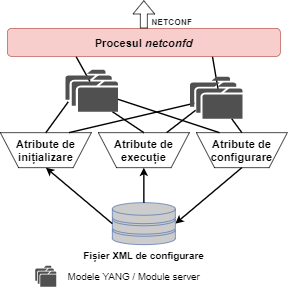
\includegraphics{dvm_v02_architecture}
	\caption{Arhitectura simulatorului DVM versiunea 2.}
	\label{fig:dvm_v02_architecture}
\end{figure}

Parametrii de iniţializare reprezintă acele atribute statice, care sunt citite din dispozitiv o singură dată, în momentul inițializării simulatorului. În cadrul serverului \gls{netconf} pot fi doar citite, în cazul parametrilor care reprezintă capabilitățile echipamentului (adică informaţie statică, prezentată de către dispozitiv, care nu se poate schimba) sau pot fi și scrise și citite, ca în cazul parametrilor de configurare. În momentul inițializării \gls{dvm} aceștia sunt consideraţi parametri de iniţializare, ca apoi să devină de configurare, având câte o funcție cu apel invers asociată, care permite modificarea acestei valori în fişierul \gls{xml} de configurare prin intermediul serverului \gls{netconf}. Nu este nevoie ca aceste atribute de configurare să fie citite din dispozitiv decât în momentul inițializării, deoarece apoi se presupune că orice configurare asupra dispozitivului se va face prin echipamentul de control \gls{sdn}, deci prin intermediul serverului \gls{netconf} care va fi astfel informat asupra noii valori a parametrilor respectivi.

Atributele de execuţie reprezintă parametrii dinamici, care pot fi doar citiţi ai dispozitivului, precum alarme, informații de stare sau de monitorizare a performanţelor. Acestea trebuie citite din echipament de fiecare dată când controlerul \gls{sdn} le cere, din cauza naturii lor dinamice. Soluția acestei abordări constă în nodurile virtuale oferite de soluția \textit{OpenYuma}. În loc de a avea o valoare stocată pentru un atribut \gls{yang}, sau valori pentru grupuri de atribute, \textit{OpenYuma} oferă posibilitatea de a asocia o funcție cu apel invers pentru astfel de parametri. Aceasta va fi apelată de fiecare dată când valoarea atributului asociat este cerută serverului \gls{netconf}, iar implementarea acesteia va prelua valoarea din fişierul \gls{xml} de configurare, sau va construi arborele asociat răspunsului, în cazul unui grup de atribute.

Cea de-a doua versiune a simulatorului \gls{dvm} se bazează pe abordarea \textit{OpenYuma} de a folosi funcții cu apel invers pentru implementarea funcţionalităţii de citire sau scriere asociată atributelor modelelor \gls{yang}. Proiectarea \gls{dvm} urmăreşte separarea descrisă anterior a parametrilor, oferind diferite funcții cu apel invers pentru diferitele categorii. Fiecare atribut din modelele \gls{yang} va fi modelat ca un nod \textit{OpenYuma}, care reprezintă un tip de date pus la dispoziţie de această soluție software, conţinând diverse informații rezultate din analizarea modelului \gls{yang}, precum numele, constrângeri asupra valorilor pe care atributul le poate lua și funcţia cu apel invers asociată, de citire sau de scriere. Astfel, au fost considerate trei funcții cu apel invers generice, care să fie folosite în cele trei cazuri date de împărțirea atributelor \gls{yang}: pentru parametrii de iniţializare, de execuţie și de configurare. Acestea sunt considerate generice, deoarece o singură astfel de funcție cu apel invers este utilizată pentru fiecare tip de atribut, diferenţierea pentru fiecare atribut în parte făcându-se în implementarea acesteia, în funcție de numele atributului. Această abordare oferă flexibilitate și uşurinţă în implementarea simulatorului \gls{dvm}.


\section{Implementarea DVM versiunea 2}

Istoria reţelelor definite prin software.
\section{Folosirea în contextul demonstraţiilor de concept a DVM versiunea 2}

Așa cum prima versiune a \gls{dvm} a fost foarte importantă în contextul celei de-a doua demonstraţii de concept a rețelelor de transport de date fără fir și a doua versiune a acestui simulator a fost o unealtă critică pentru pregătirea celei de-a treia demonstraţii de concept. A permis dezvoltatorilor de aplicații \gls{sdn} să le testeze și să le depaneze într-o manieră facilă, eliminând necesitatea deţinerii unor echipamente de rețea și a mediatorului asociat.

\gls{sdn} nu influenţează doar modul în care rețelele sunt controlate și administrate, ci și modul în care sunt organizate proiectele și modul în care anumite cerinţe și capabilităţi sunt dezvoltate și implementate. Dacă înainte aplicațiile și dispozitivele de rețea erau oferite împreună, de către producătorii de echipamente, interfeţele standard dintre dispozitive și echipamentele de control \gls{sdn}, sau dintre echipamentele de control și aplicații, oferă posibilitatea companiilor de a oferi doar anumite secţiuni din întreaga soluție. Aceste companii pot profita de simulatorul \gls{dvm}, deoarece le oferă acces la aceste interfețe fără a avea nevoie să deţină echipamente de rețea foarte scumpe.

Avantajul pe care \gls{dvm} îl oferă și care a fost folosit în cea de-a treia demonstraţie de concept \gls{onf} este reprezentat de faptul că orice modificare în modelele \gls{yang} dezvoltate poate fi testată cu ajutorul simulatorului, deoarece acesta oferă o modalitate rapidă de a o implementa, simulând astfel, din punctul de vedere al echipamentului de control \gls{sdn}, interacţiunea cu un dispozitiv de rețea. După dezvoltarea simulatorului și a aplicațiilor \gls{sdn}, acestea din urmă pot fi testate, chiar înainte ca software-ul din elementele de rețea să fie implementat. Cu toate acestea, este nevoie ca aplicațiile să efectueze teste de integrare cu dispozitivele de rețea, deoarece comportamentul simulatorului nu poate fi identic cu cel al echipamentelor. Simulatorul \gls{dvm} folosit în cea de-a treia demonstraţie de concept nu a simulat dispozitivele de rețea, ci nivelul mediator care oferă interfaţa \gls{netconf} ce expune modelele \gls{yang} dorite. A fost posibilă simularea diferitor topologii de rețea, având dispozitive cu diferite configurări și interfețe de transport de date. Simulatorul \gls{dvm} a fost și în cazul celor de-a doua și de-a treia demonstraţii de concept \gls{onf} unealta principală pentru a putea crea o topologie de rețea simulată \cite{onf2016_poc2, onf2016_poc3}. 

Simulatorul a fost folosit și pentru teste de extensibilitate și de performanţă ale aplicațiilor \gls{sdn} dezvoltate. Fişierul \gls{xml} de configurare poate fi manipulat foarte uşor, adăugând interfețe de transport de date echipamentelor sau intrări pentru valorile indicatorilor de performanţă. De exemplu, un dispozitiv de rețea are nevoie de 24 de ore pentru a genera 96 de intrări ale indicatorilor de performanţă de 15 minute și 30 de zile pentru a genera 30 de intrări ale indicatorilor de performanţă de 24 de ore. O altă funcție importantă a \gls{dvm} care a fost folosită în pregătirea demonstraţiei de concept a fost cea de generare a notificărilor \gls{netconf}. Au putut fi simulate diferite tipuri de notificări care să apară la un interval de timp configurabil.

În mod evident, timpii de răspuns ai simulatorului sunt foarte reduşi, deoarece nu există o comunicaţie cu un echipament de rețea real, deci nici nevoia de a procesa valorile atributelor care sunt citite din dispozitivele de rețea. Nevoia de a procesa valorile unor atribute apare în cazul mediatoarelor reale, în momentul în care atributele definite în modelul informațional pentru microunde nu se potrivesc în totalitate cu atributele dispozitivului și o anume procesare a acelei valori este necesară pentru a transforma-o în ce se doreşte în modelul \gls{yang}.

Tabelul \ref{tab:Table_3} ilustrează diferenţele între \gls{dvm} și un mediator real, în diferite situaţii care au apărut în pregătirea celei de-a treia demonstraţii de concept \gls{onf} \cite{stancu2017enabling}.

\begin{table}[h]
	
	\caption{Comparaţie între comportamentele unui mediator real și al simulatorului în diferite situații \cite{stancu2017enabling}.\label{tab:Table_3}}
	\begin{tabular}{|M{0.5\textwidth}|M{0.2\textwidth}|M{0.2\textwidth}|}
		\hline
		\textbf{Situația} & \textbf{\emph{Mediator real}} & \textbf{\emph{Simulatorul DVM}} \tabularnewline
		\hline 
		Dezvoltarea aplicațiilor \gls{sdn} & costisitoare & eficientă \tabularnewline
		\hline 
		Timpul de implementare & greoi & rapid \tabularnewline
		\hline 
		Topologia de rețea & complex de schimbat & flexibilă, uşor de schimbat \tabularnewline
		\hline 
		Generarea notificărilor \gls{netconf} & greu de controlat & simplă \tabularnewline
		\hline 
		Timpi de răspuns & reali & nerealişti \tabularnewline
		\hline 
		Procesare a valorilor atributelor & în unele cazuri & nu este nevoie \tabularnewline
		\hline \end{tabular}
\end{table}

Pentru a oferi un suport mai bun testelor de extensibilitate și de performanţă ale aplicațiilor, simulatorul \gls{dvm} ar fi putut implementa timpi de răspuns configurabili la operaţiile \gls{netconf} sau generarea de notificări care să urmărească anumite pofile temporale, în funcție de nevoile aplicațiilor \gls{sdn}.

La fel ca în cazul versiunii anterioare a \gls{dvm}, înregistrarea simulatoarelor la echipamentul de control \gls{sdn} se face manual, cu ajutorul interfeţei grafice a controlerului, care stabileşte apoi conexiunea securizată și iniţiază o sesiune \gls{netconf}.
\section{Integrarea DVM cu comutatorul software LINC: \textit{LINC-WE}}

Așa cum a fost descris anterior, simulatorul \gls{dvm} permite emularea nivelului mediator care apare în arhitectura \gls{sdn} a rețelelor de transport de date fără fir. Se pot simula diferite topologii de rețea prin manipularea fişierelor \gls{xml} de configurare ale diferitelor instanţe ale \gls{dvm}, făcând simulatoarele să prezinte diferite configuraţii. Această abordare oferă un bun prim pas pentru simularea rețelelor de transport de date fără fir în contextul \gls{sdn}, însă nu este suficient, deoarece instanţele \gls{dvm} sunt independente și rețeaua simulată nu este completă. În plus, nu există legături între dispozitivele simulate. Din acest motiv, această secţiune prezintă încercarea de a integra simulatorul \gls{dvm} cu un comutator software deja existent, care a fost folosit anterior pentru simulări de rețele optice în contextul \gls{sdn}: \textit{Legătura Nu Este Închisă} - \gls{linc} și cu simulatorul de rețele definite prin software, \textit{mininet}. Comutatorul software folosit anterior în simularea rețelelor optice~\cite{parulkar2015sdn, kretsis2016emulation, mehmeri2017software}, bazat pe \gls{linc} se numeşte \textit{Legătura Nu Este Închisă - Extensii Optice} - \gls{linc-oe}, astfel că am denumit comutatorul rezultat în urma integrării \gls{dvm} cu \gls{linc}: \textit{Legătura Nu Este Închisă - Emulator Fără Fir} - \gls{linc-we}~\cite{stancu2017wireless}.

\subsection{LINC}

\gls{linc} este un comutator software ce suportă protocolul OpenFlow, scris în limbajul de programare Erlang~\cite{lincsw}. Acesta a fost proiectat să fie modular, oferind o metodă rapidă de a face prototipuri \gls{sdn} și de a testa noi caracteristici ale protocolului OpenFlow. Este oferit ca o implementare cu sursă deschisă de către \textit{FlowForwarding.org} și are ca scop oferirea unei soluții prin care utilizatorii pot evalua rapid protocoalele OpenFlow și OF-Config.

Un singur comutator este implementat ca un nod Erlang și cuprinde mai multe comutatoare logice. Acestea, porturile și legăturile dintre porturi sunt descrise de către utilizator prin intermediul unui fișier de configurare, așa cum este ilustrat și în Figura \ref{fig:linc_architecture}. Datorită acestei arhitecturi modulare, comutatorul \gls{linc} este capabil să ofere mai multe implementări pe care utilizatorul le poate alege, fiecare având asociată o versiune diferită a protocolului OpenFlow (versiunile 1.2, 1.3 sau 1.4). Aceste implementări sunt responsabile de comutarea pachetelor și modificarea tabelelor de fluxuri de date.

\begin{figure}[h]
	\centering
	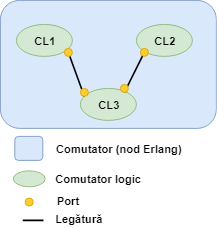
\includegraphics{linc_architecture}
	\caption{Arhitectura comutatorului software LINC~\cite{linc2014qsg}.}
	\label{fig:linc_architecture}
\end{figure}

După cum este prezentat în~\cite{linc2014qsg}, \gls{linc} prezintă mai multe blocuri software: comutatorul capabil OpenFlow, modului protocolului OpenFlow, modului protocolului OF-Config. Acestea sunt dezvoltate ca aplicații Erlang separate, respectând principiile \textit{Platforma Telecom Deschisă} - \gls{otp} ale limbajului Erlang. Există și o componentă separată care se ocupă de conexiunea la un echipament de control \gls{sdn}. Tabelele de fluxuri, porturile sau tabelele de grup sunt administrate de implementările separate reprezentând diferitele versiuni ale protocolului OpenFlow.

\subsubsection{LINC-OE}

Datorită naturii modulare a comutatorului \gls{linc}, a apărut o nouă implementare care să acopere cazurile de utilizare ale \gls{sdn} din domeniul optic: \gls{linc-oe} \cite{parulkar2015sdn}. Acesta reprezintă un simulator de comutatoare optice care suportă extensiile optice ale protocolului OpenFlow. Diferenţa dintre \gls{linc} și \gls{linc-oe} este că, în cazul celui din urmă, comutatoarele logice care sunt simulate reprezintă comutatoare optice, astfel încât spre deosebire de interfeţele electrice, porturile optice oferă mai multe canale de comunicaţie independente, diferenţiate prin lungimea de undă. În implementarea \gls{linc-oe}, mesajele ce se transmit printr-un astfel de port optic nu mai sunt pachete Ethernet, ci mesaje Erlang, ce conţin informații adiţionale, pe lângă pachetul Ethernet propriu-zis. O altă diferenţă este dată de faptul ca \gls{linc-oe} oferă interfețe pentru simularea defectării legăturilor dintre porturi.

\subsubsection{Interfaţa NETCONF}

Comutatorul software \gls{linc} include de asemenea și o interfață \gls{netconf}. Este folosită de către protocolul OF-Config și este disponibilă pentru un comutator doar dacă acel protocol este folosit. În cazul în care este permisă utilizarea acestuia, o nouă aplicație Erlang este pornită în cadrul nodului Erlang: \textit{enetconf}, care pornește un server \gls{netconf} ce aşteaptă conexiuni pe adresa \gls{ip} și portul selectate de utilizator.

Această abordare prezintă un dezavantaj major: doar un singur server \gls{netconf} este pornit pentru comutatorul \gls{linc}, astfel că nu se pot accesa comutatoarele logice care alcătuiesc comutatorul \gls{linc} individual prin interfaţa \gls{netconf}. Acestea pot fi configurate doar prin intermediul protocolului OpenFlow \cite{lincsw}.

De asemenea, modelul informațional \gls{yang} care este oferit de către server nu este configurabil, astfel încât utilizatorul nu poate alege un model \gls{yang} pe care comutatorul software să îl poată folosi. Dacă acest lucru ar fi fost oferit, ar fi fost banală transformarea \gls{linc-oe} în \gls{linc-we}, prin înlocuirea modelului \gls{yang} expus cu modelul informațional pentru microunde și apoi corelarea atributelor \gls{yang} cu parametrii comutatorului \gls{linc}.

\subsection{LINC-WE}

\gls{linc-we} a apărut ca o încercare de a îmbunătăţi simulatorul \gls{dvm} dezvoltat anterior, prin oferirea unei soluții care să simuleze nu doar dispozitive de rețea independente, ci și legăturile dintre acestea. Astfel, am luat în considerare integrarea \gls{dvm} cu un comutator software deja existent, \gls{linc}, având în vedere și faptul că acesta a fost folosit anterior pentru simularea de rețele optice în contextul \gls{sdn}, prin \gls{linc-oe} \cite{parulkar2015sdn}.

Spre deosebire de \gls{linc} și \gls{linc-oe}, \gls{linc-we} nu ilustrează utilizarea protocolului OpenFlow pentru configurarea comutatorului, ci pune accent pe protocolul \gls{netconf} pentru administrarea dispozitivelor de rețea. Oferă totuşi suportul pentru protocolul OpenFlow, prin modulele \gls{linc} care implementează versiunile 1.2, 1.3 și 1.4 ale acestuia. Deoarece configurarea și administrarea dispozitivelor de transport de date fără fir a migrat de la protocolul OpenFlow (prin dezvoltarea de extensii specifice) la \gls{netconf}, așa cum demonstrează activitatea de cercetare din cadrul \gls{onf}, prin apariția modelelor informaționale care pot fi ușor transformate în modele \gls{yang} \cite{onftr532, onftr512v1.0, onftr512v1.1, onftr512v1.2}, această abordare oferind mai multă flexibilitate. \gls{linc-we} încearcă să construiască pe această bază prin oferirea unui comutator software care să expune modelele \gls{yang} propuse de \gls{onf} și să poată fi folosit în simulări.

Abordarea aleasă în acest caz a fost înlocuirea aplicaţiei Erlang \textit{enetconf}, care implementa serverul \gls{netconf} pentru comutatorul software \gls{linc} cu o aplicație externă, dezvoltată în C, care să expună modelele \gls{yang} specifice rețelelor de transport de date fără fir: \gls{dvm}.

Implementarea serverului \gls{netconf} este dată de simulatorul descris anterior, \gls{dvm}. Pentru integrarea acestuia cu comutatorul software \gls{linc} am înlocuit aplicaţia Erlang ce implementa suportul pentru acest protocol, \textit{enetconf}, cu o aplicație Erlang nouă, dezvoltată în acest scop: \textit{erl\_yuma}. Aceasta se ocupă de pornirea și oprirea serverului \gls{netconf} implementat pentru \gls{dvm}, prin deschiderea unui port Erlang care va avea această sarcină. Codul acestei soluții este oferit cu sursă deschisă și poate fi găsit pe platforma GitHub~\cite{lincwe2017}.

Din punctul de vedere al echipamentului de control \gls{sdn}, acesta va comunica prin interfaţa \gls{netconf} cu \gls{dvm}, care a fost pornit anterior din mediul Erlang (prin aplicaţia \textit{erl\_yuma}). Comunicaţia dintre aplicațiile dezvoltate în Erlang și în C este administrată de către sistemul de execuţie Erlang. Din perspectiva \textit{erl\_yuma}, comunicaţia cu \gls{dvm} se face prin mesaje standard Erlang, care sunt transmise prin portul Erlang asociat acesteia. Din cealaltă perspectivă, a \gls{dvm}, comunicaţia se realizează prin fluxurile standard de intrare și de ieșire, \textit{stdin} și \textit{stdout}. O imagine de ansamblu a arhitecturii \gls{linc-we} este prezentată în Figura \ref{fig:linc_we_architecture}.

\begin{figure}[h]
	\centering
	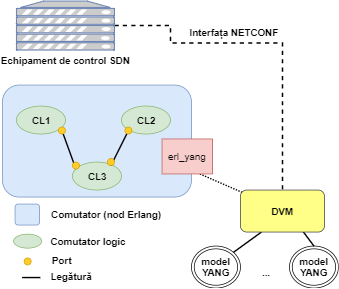
\includegraphics{linc_we_architecture}
	\caption{Arhitectura comutatorului software LINC-WE~\cite{linc2014qsg}.}
	\label{fig:linc_we_architecture}
\end{figure}

Restul arhitecturii \gls{linc} nu este influenţată: există în continuare comutatorul software, care expune o interfață \gls{netconf} (doar că acum este oferită prin \gls{dvm}) și conţine mai multe comutatoare logice, împreună cu porturile acestora și legăturile dintre ele, așa cum a fost definit în fişierul de configurare \gls{linc}. Aplicaţia ce oferă interfaţa \gls{netconf}, \textit{erl\_yuma}, este pornită doar în cazul în care protocolul OF-Config este activat.

\subsubsection{Interfața NETCONF - Aplicația Erlang}

Aplicaţia care transformă comutatorul software \gls{linc} în \gls{linc-we}, prin integrarea cu \gls{dvm} este \textit{erl\_yuma}. Aceasta este o aplicație Erlang tipică, ce respectă principiile \gls{otp} \cite{logan2010erlang}.

Structura aplicaţiei respectă recomandările \gls{otp}. În dosarul rădăcină \textit{erl\_yuma} al aplicaţiei sunt create următoarele directoare: \textit{ebin}, ce conţine fişierele compilate *.beam, dar și fişierul de resurse ale aplicaţiei \gls{otp} (ce conţine informații precum descrierea, versiunea, etc.). Directoarele \textit{include} și \textit{priv} ar trebui să conţină fişierele de incluziune *.hrl și respectiv aplicațiile externe de care depinde aplicaţia Erlang. Încă două dosare alcătuiesc aplicaţia: \textit{src}, unde se găsesc fişierele sursă și \textit{test}, ce conţine fişiere de test.

O imagine de ansamblu a aplicaţiei Erlang poate fi văzută în Figura \ref{fig:erlang_application}. Există trei fişiere sursă importante: \textit{ey\_app.erl}, \textit{ey\_sup.erl} și \textit{ey\_server.erl}.

\begin{figure}[h]
	\centering
	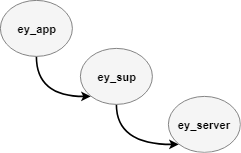
\includegraphics{erlang_application}
	\caption{Structura aplicației Erlang \textit{erl\_yuma}~\cite{linc2014qsg}.}
	\label{fig:erlang_application}
\end{figure}

Primul fişier sursă, \textit{ey\_app.erl}, reprezintă implementarea unui comportament \textit{aplicație}, așa cum este definit în \gls{otp}. Este o implementare simplă și directă a acestui comportament \gls{otp}, care oferă doar două funcții cu apel invers: \textit{start} și \textit{stop}. Prima este folosită pentru a porni procesul care este responsabil pentru implementarea aplicaţiei. Acesta este un proces \gls{otp} supervizor.

Cel de-al doilea fişier sursă, \textit{ey\_sup.erl}, implementează un comportament \textit{supervizor} definit de \gls{otp}. Acesta este procesul central al aplicaţiei \textit{erl\_yuma} și este responsabil pentru supravegherea acestuia. Este necesară implementarea unei singure funcții cu apel invers oferite de acest comportament: \textit{init}. În momentul în care procesul supervizor este pornit, această funcție este invocată, acesta fiind și locul în care ar trebui să pornim procesul \textit{ey\_server.erl}, conform cu structura aplicaţiei noaste. Nu trebuie să pornim mai multe procese copil în acest punct, deoarece dorim să expunem o singură interfață \gls{netconf}. Astfel, procesul supervizor va porni un singur modul \textit{ey\_server}.

Ultimul fişier sursă care alcătuieşte aplicaţia \textit{erl\_yuma} este \textit{ey\_server.erl}. Din punctul de vedere \gls{otp}, acest modul implementează un comportament \textit{gen\_server} (server generic). Acest proces este responsabil de crearea unui port Erlang, care porneşte aplicaţia externă C, reprezentată de \gls{dvm}. Astfel, procesul va stoca portul care a fost creat. În funcţia cu apel invers \textit{init}, practic însemnând atunci când procesul este pornit, un port Erlang este creat. Intern, acest lucru înseamnă crearea unui nou proces, bazată pe o anumită comandă. Comanda este definită ca o variabilă de mediu și este stocată în fişierul de resurse ale aplicaţiei și reprezintă de fapt comanda necesară pornirii \gls{dvm}. A fost folosită această abordare pentru a fi uşor de modificat în cazul în care comanda cu care se porneşte \gls{dvm} se va schimba pe viitor. Astfel, aplicaţia Erlang nu va trebui recompilată.

Un aspect interesant îl constituie modalitatea în care portul Erlang trebuie închis. Când utilizatorul doreşte închiderea \gls{linc-we}, trebuie ca și \gls{dvm} să fie închis, astfel încât să fie pregătit pentru o eventuală viitoare rulare. Acest lucru se face prin implementarea funcţiei cu apel invers \textit{terminate} a modulului \textit{ey\_server}. Este important de menţionat faptul că pentru ca această funcție să fie invocată în momentul închiderii aplicaţiei, aceasta trebuie să proceseze mesaje capcană (\textit{trap message}). Implementarea funcţiei \textit{terminate} va trebui să închidă instanţa \gls{dvm} care rulează (prin trimiterea unui semnal de închidere a procesului către sistemul de operare).

În prima versiune a \gls{linc-we} nu a fost implementată comunicaţia dintre aplicațiile Erlang și C. Cu ajutorul acesteia s-ar fi putut manipula parametrii comutatorului software, prin operații \gls{netconf}. Practic, \gls{linc-we} doar crează o instanţă un simulator \gls{dvm}, expunând o interfață \gls{netconf}, care însă nu implementează și modificarea atributelor comutatorului \gls{linc}.

\subsection{Concluziile integrării}

O unealtă ce oferă posibilitatea de a simula rețele ce conţin dispozitive de transport de date fără fir, care să expună și modelul informațional pentru microunde propus de \gls{onf} este importantă atât pentru membrii \gls{onf}, care pot testa, revizui și îmbunătăţi modelul, cât și pentru dezvoltatorii de aplicații \gls{sdn} care pot începe implementarea și testarea de software pentru astfel de rețele. Deoarece TR-532 a fost propus de curând, în decembrie 2016, nu există încă suport pentru acesta în simulatoare de rețea consacrate, precum OPNET sau OMNeT++, făcând \gls{linc-we} prima încercare de simulator care să ofere o astfel de interfață unui echipament de control \gls{sdn}.

\gls{linc-we} oferă posibilitatea unei lansări rapide a unui simulator ce suportă modelul TR-532 și, spre deosebire de \gls{dvm}, care era oferea doar serverul \gls{netconf} ce expunea modelele informaționale \gls{onf}, oferă și posibilitatea de a transmite trafic de date prin rețeaua simulată. Acest lucru este posibil deoarece \gls{linc-we} se bazează pe soluţia deja existentă și folosită în rețele optice, \gls{linc-oe}. Parte din cercetarea anterioară a fost și integrarea \gls{linc-oe} cu simulatorul de rețele definite prin software, \textit{mininet}, astfel că și \gls{linc-we} va fi integrat implicit cu această unealtă.

Această abordare a permis o integrare rapidă a \gls{linc} cu \gls{dvm}. După parcurgerea etapei destul de greoaie de învăţare a limbajului de programare Erlang, în care este implementat comutatorul software \gls{linc}, integrarea cu \gls{dvm} a fost facilă, aplicaţia Erlang ce se ocupă de acest aspect, descrisă anterior, fiind destul de simplă. Aceasta respectă principiile \gls{otp} și porneşte instanţa \gls{dvm} ce expune modelele \gls{yang} dorite.

Un alt avantaj oferit de această soluție este faptul că \gls{linc-we} oferă atât suport pentru protocolul \gls{netconf}, cât și pentru protocolul OpenFlow. Astfel, un echipament de control \gls{sdn} poate folosi, pe de o parte, interfaţa \gls{netconf} pentru a configura parametrii dispozitivelor simulate și, pe de altă parte, interfaţa OpenFlow pentru a administra traficul din rețea prin manipularea tabelelor de fluxuri ale echipamentelor.

Principalul dezavantaj al abordării folosite în cadrul \gls{linc-we} este faptul că poate oferi o singură interfață \gls{netconf}, care este asociată cu comutatorul software și nu câte o interfață \gls{netconf} pentru fiecare comutator logic din interiorul topologiei. Soluția evidentă ar fi pornirea câte unei aplicații \textit{erl\_yuma} pentru fiecare astfel de comutator, însă aceasta nu este banală și uşor de implementat, deoarece \gls{dvm} nu este proiectat să ruleze mai multe instanţe pe aceeaşi mașină, având anumite lucruri ce nu pot fi împărţite (de exemplu portul pe care aşteaptă conexiuni serverul \gls{netconf}, sau fişierul \gls{xml} de configurare).

Un alt dezavantaj îl constituie faptul că \gls{linc-we} nu este uşor de utilizat. Trebuie urmaţi mai mulți paşi înainte ca acesta să poată fi pornit: instalarea comutatorului software \gls{linc}, care implică instalarea mediului Erlang în prealabil; apoi, simulatorul \gls{dvm} trebuie instalat, după ce a fost instalată anterior soluţia software OpenYuma.

Fiind doar prima versiune a \gls{linc-we}, a fost implementată rapid pentru a putea fi folosită pentru teste. Asta înseamnă că se pot aduce multe îmbunătăţiri acestei soluții. Un aspect important ce ar putea fi luat în considerare este asocierea parametrilor din modelul informațional pentru microunde cu parametri reali din comutatorul software. Asta implică, însă, o înţelegere mai aprofundată a limbajului de programare Erlang. Implementarea comutatorului \gls{linc} ar putea ţine cont de aceşti parametri în simulare. De exemplu, dacă frecvenţele emiţătoarelor și receptoarelor unor porturi care comunică nu se potrivesc, comunicarea între acestea ar putea fi oprită în implementarea comutatorului.

Dată fiind dificultatea limbajului de programare Erlang și limitările descrise anterior, am renunţat la dezvoltarea unei a doua versiuni a \gls{linc-we} și am căutat o alternativă la această abordare care să fie mai facilă și mai uşor de dezvoltat și implementat. Soluția găsită a fost folosirea unei unelte de creare a unor containere software care pot rula într-un mod izolat anumite aplicații: \textit{docker}. Aceasta va fi detaliată în capitolul următor.
\chapter{Mediatorul cu valori implicite (DVM) - a doua versiune\label{ch:dvm_v02}}

\section{Arhitectura}

SDN și reţelele actuale..
\section{Implementarea}

Istoria reţelelor definite prin software.
\section{Folosirea în contextul demonstraţiilor de concept}

Standardizare: ONF, etc..
\section{LINC-WE. Integrarea cu \textit{mininet}}

Standardizare: ONF, etc..

\chapter{Simulatorul reţelelor de transport de date fără fir (WTE)\label{ch:wte}}

\section{Arhitectura}

Simulatorul rețelelor de transport de date fără fir a fost proiectat pentru a rula pe o singură mașină Linux și să simuleze acolo o topologie de rețea, folosind diferite unelte. Scopul simulatorului a fost să expună în continuare modelele informaționale de bază și pentru microunde, precum versiunea precedentă, \gls{dvm}. Astfel, există un fişier de configurare în care se specifică topologia ce se vrea a fi simulată, în limbajul \textit{Notaţie de Obiecte JavaScript} - \gls{json}. Formatul acestui fişier de topologie este unul fix și este influenţat de către nivelurile de transport ale obiectelor \gls{ltp} definite în modelul informațional de bază. Mai multe detalii despre acest format vor fi date în secţiunea următoare.

Există mai multe unelte care sunt folosite în arhitectura \gls{wte}, care împreună alcătuiesc simulatorul. Fiecare dispozitiv de rețea este simulat printr-un container \textit{docker}, în care rulează o imagine \textit{Linux} și serverul \gls{netconf} reprezentat de \gls{dvm}. Această abordare a fost aleasă pentru a obţine o izolare la nivelul sistemului de fişiere, astfel încât mai mule instanţe ale \gls{dvm} să poată funcţiona fără probleme pe aceeaşi mașină. Interfețele prezente în fiecare echipament sunt reprezentate prin interfețe de rețea în imaginea Linux, iar legăturile dintre dispozitive se fac cu ajutorul acestora. Fiecare element de rețea are o interfață de administrare, prin care se conectează la echipamentul de control \gls{sdn}. Pentru a obţine o izolare a acestor interfețe (mai exact pentru ca traficul de date care ar putea fi transmis prin interfeţele unui dispozitiv să nu tracă prin interfaţa de administrare), astfel încât echipamentele să nu comunice între ele prin aceste interfețe, au fost folosite \textit{rețelele docker}. Toate aceste elemente sunt ilustrare în Figura \ref{fig:wte_architecture} și vor fi detaliate în continuare.

\begin{figure}[h]
	\centering
	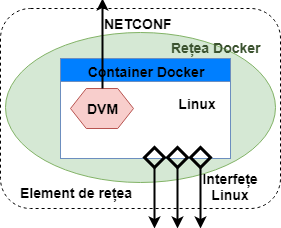
\includegraphics{wte_architecture}
	\caption{Arhitectura WTE.}
	\label{fig:wte_architecture}
\end{figure}

\textit{Docker} este o unealtă care permite crearea de containere software în care pot rula aplicații într-un mod izolat față de aplicațiile sistemului de operare gazdă, care lansează aceste containere \cite{merkel2014docker}. Acestea permit împachetarea unei aplicații într-un container \textit{docker}, împreună cu toate aplicațiile software de care ea depinde. Consumul de resurse al unui astfel de container este mult mai redus decât al unei mașini virtuale, deoarece nu se replică tot sistemul de operare, ci doar bibliotecile și procesele necesare aplicaţiei care este virtualizată. După cum este prezentat și în \cite{chamberlain2014using}, \textit{docker} poate fi utilizat și pentru a produce activitate de cercetare reproductibilă. Astfel, această unealtă este folosită și în cazul \gls{wte} pentru a obţine izolarea, la nivelul sistemului de fişiere al maşinii gazdă, a aplicaţiei ce implementează serverul \gls{netconf} ce expune modelele informaționale dorite: \gls{dvm}.

\textit{Rețelele docker} reprezintă o facilitate oferită de soluţia \textit{docker} prin care se poate izola și stiva de rețea asociată unei imagini \textit{docker}. Astfel, un container poate fi asociat unei \textit{rețele docker} și imaginile ce aparţin unor \textit{rețele docker} diferite sunt izolate și din punctul de vedere al comunicației dintre ele. Un utilizator își poate crea diferite \textit{rețele docker}, având adrese de rețea sau spaţii de adrese la alegere.

Din punctul de vedere al legăturilor ce se pot face între aceste containere, mai exact între interfeţele Linux ce fac parte din imaginile \textit{docker} care reprezintă elementele de rețea, au fost considerate două abordări, care vor fi descrise în secțiunea următoare. În prima abordare, s-a încercat folosirea unui comutator software prin intermediul căruia să se facă conexiunile, \textit{Comutatorul Virtual Deschis} - \gls{ovs}. Cea de-a doua abordare constă în crearea unei conexiuni între aceste interfețe printr-o \textit{pereche Ethernet virtuală (virtual ethernet pair - \textbf{veth})}. %Diferenţele între cele două abordări vor fi detaliate în secţiunea următoare.

%\begin{figure}[h]
%	\centering
%	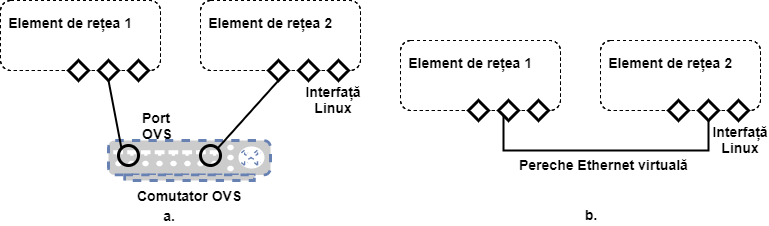
\includegraphics[width=1\textwidth]{wte_links}
%	\caption{Legăturile între dispozitivele de rețea simulate în WTE: a) prin OVS; b) prin \textit{veth}.}
%	\label{fig:wte_links}
%\end{figure}

În urma proiectării \gls{wte} a rezultat o abordare simplă: în momentul inițializării, simulatorul ar trebui să analizeze fişierul care conţine topologia ce trebuie simulată. Apoi, ar trebui să construiască \textit{rețelele docker} asociate fiecărui dispozitiv de rețea definit în topologie și să pornească imaginile \textit{docker} necesare, să creeze interfeţele Linux asociate cu diferitele niveluri de transport ale obiectelor \gls{ltp} definite în topologie, după care să construiască legăturile dintre aceste interfețe.

Componentele care alcătuiesc \gls{wte} sunt prezentate în Figura \ref{fig:wte_components} și sunt următoarele: \gls{dvm}, care a fost adaptat pentru a putea funcţiona în mediul propus de \gls{wte}, fişierul \gls{json} care conţine topologia ce trebuie simulată, fişierul care conţine detalii despre cum ar trebui să fie configurat \gls{wte}, comutatorul software \gls{ovs} (doar în cazul primei abordări propuse pentru reprezentarea legăturilor dintre două elemente de rețea) și un cadru software care să pună toate componentele împreună și să implementeze logica simulatorului. Această ultimă componentă este scrisă în limbajul Python și reprezintă nucleul \gls{wte}.

\begin{figure}[h]
	\centering
	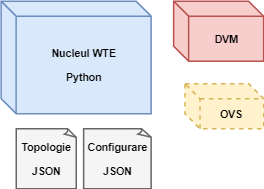
\includegraphics{wte_components}
	\caption{Componentele majore ale WTE.}
	\label{fig:wte_components}
\end{figure}

Nucleul \gls{wte} care este scris în limbajul Python este responsabil pentru implementarea infrastructurii de care simulatorul are nevoie și este proiectat să fie modular și flexibil. Este dezvoltat într-o manieră orientată pe obiecte, având clase pentru fiecare componentă importantă de care este nevoie: cadrul general al simulatorului, elementele de rețea, legăturile de date, topologia, etc. Aceasta oferă posibilitatea de extindere folosind, de exemplu, altă soluție care să implementeze un server \gls{netconf}.
\section{Implementarea}

Implementarea \gls{wte} se bazează pe cod scris în limbajele Python, pentru nucleul simulatorului, ce implementează infrastructura și pe cod scris în limbajul C, pentru serverul \gls{netconf}, soluţia \gls{dvm} ce a fost dezvoltată anterior fiind adaptată pentru noua abordare. Codul este oferit cu sursă deschisă și poate fi găsit pe platforma GitHub~\cite{wte2017}. Paragrafele următoare vor prezenta detalii despre implementare, evidenţiind avantajele acestei abordări și motivele pentru care soluţia poate fi considerată un adevărat simulator de rețele de transport de date fără fir. 

\subsection{Fişierele de configurare}

\gls{wte} folosește fişiere de configurare, pentru a oferi o interfață simplă de configurare utilizatorilor. Există două fişiere scrise în limbajul \gls{json}, \textit{topology.json} și \textit{config.json}, primul pentru descrierea topologiei care va fi simulată și celălalt pentru a descrie caracteristicile configurabile ale simulatorului. Din aceeaşi categorie fac parte și modelele informaționale. Fişierele \gls{yang} asociate acestora sunt folosite de către simulator pentru a fi expuse de serverul \gls{netconf}.

Fişierul \gls{json} care descrie topologia are un format static, ce va fi prezentat în continuare. Acesta este ilustrat și în Figura~\ref{fig:wte_topology_json}.

\begin{figure}[h]
	\centering
	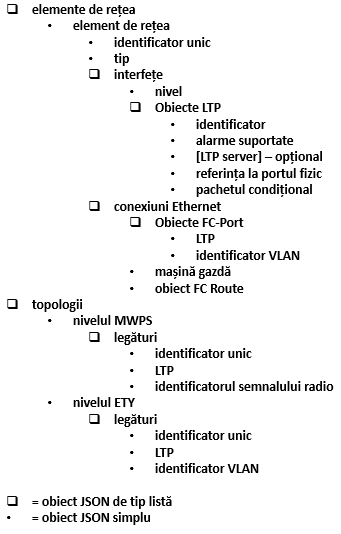
\includegraphics{wte_topology_json}
	\caption{Formatul fișierului JSON care descrie topologia rețelei simulată cu WTE.}
	\label{fig:wte_topology_json}
\end{figure}

Pentru descrierea topologiei unei rețele este suficient să cunoaştem dispozitivele și legăturile dintre acestea. Fiind rețele de transport de date fără fir, în cele mai simple cazuri, putem avea două tipuri de legături între echipamente: fără fir, sau legături Ethernet. Astfel, fişierul de topologie conţine două obiecte \gls{json} de tip listă: (i) \textbf{elemente de rețea} (\textit{network-elements}), ce descrie dispozitivele de rețea și (ii) \textbf{topologii} (\textit{topologies}), reprezentând legăturile dintre echipamente.

Fiecare element de rețea va avea mai multe detalii prezente în fişierul de topologie. Identificatorul unic reprezintă un nume unic ce va fi dat fiecărui dispozitiv de rețea, pentru a-l putea recunoaşte în topologia simulată. Tipul elementului se referă la soluţia ce va fi folosită pentru implementarea serverului \gls{netconf} ce va expune modelele informaționale dorite. În cazul alegerii \gls{dvm}, valoarea acestui element este \textit{OpenYuma}. Pentru cea de-a patra demonstraţie de concept \gls{onf}, o companie a folosit simulatorul \gls{wte} pentru dezvoltarea de aplicații \gls{sdn}, dar a preferat o soluție mai simplă, dar cu mai puţine capabilităţi pentru implementarea serverului \gls{netconf}, astfel că a folosit acest parametru pentru a informa nucleul simulatorului să folosească celălalt server. 

Elementul cel mai important al unui dispozitiv de rețea este reprezentat de obiectul \gls{json} de tip listă \textit{interfețe}, fiind responsabil pentru descrierea interfeţelor acelui dispozitiv. O interfață a unui echipament are ca echivalent un obiect \gls{ltp} din modelul informațional de bază. Obiectul \textit{nivel} din lista de interfețe reprezintă nivelul de transport asociat obiectului \gls{ltp}. Valorile pe care acesta le poate lua sunt descrise în modelul informațional de bază, în Capitolul~\ref{ch:sdn_in_contextul_wt}: \gls{mwps}, \gls{mws}, \gls{etc}, \gls{ety} și \gls{eth}. Fiecare interfață prezintă câteva detalii de care simulatorul are nevoie: identificatorul obiectului \gls{ltp}, alarmele suportate (simulatorul are nevoie de această valoare, deoarece în modelul informațional pentru microunde, pe baza acestui atribut este definită lista alarmelor suportate și aceasta are un număr minim elemente; dacă nu este implementat acest număr minim, modelul \gls{yang} prezentat de serverul \gls{netconf} nu va fi valid), obiectul \gls{ltp} care reprezintă serverul pentru obiectul \gls{ltp} curent, dacă există (pentru reprezentarea relaţiilor de tip client-server dintre interfețe), referinţa la portul fizic și pachetul condiţional folosit de acest obiect \gls{ltp}.

Următorul obiect \gls{json} care face parte din fişierul de descriere a topologiei este tot un obiect de tip listă, \textit{conexiuni Ethernet}. Acestea reprezintă obiectele \gls{fc} definite în modelul informațional de bază. Practic, acestea exprimă conexiunile interne între interfeţele dispozitivului (de exemplu, traficul de pe o interfaţă radio R1 va fi dirijat către o interfață Ethernet E2). De aceea, obiectul \textit{conexiuni Ethernet} conţine două obiecte de tipul porturi \gls{fc}, care descriu exact această legătură internă. Obiectul \gls{json} \textit{mașină gazdă} care este prezent aici este folosit pentru simularea unei gazde care folosește această conexiune internă și este utilizat pentru generarea sau recepţionarea de trafic în cadrul simulatorului.

Obiectul \gls{json} \textit{topologii} descrie legăturile dintre dispozitivele de rețea. Există două niveluri de transport la care pot exista aceste conexiuni: \gls{mwps}, adică legăturile fără fir și \gls{ety}, reprezentând conexiunile Ethernet dintre echipamente. Fiecare legătură este reprezentată ca un obiect \gls{json} de tip listă, având doar două elemente, ce descriu cele două capete ale conexiunii, prin identificatorul unic al dispozitivului și identificatorul unic al interfeţei.

Cel de-al doilea fişier \gls{json} folosit de \gls{wte} este \textit{config.json}. Formatul acestuia poate fi observat în Figura~\ref{fig:wte_config_json}.

\begin{figure}[h]
	\centering
	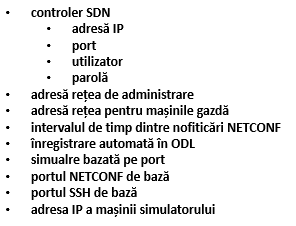
\includegraphics{wte_config_json}
	\caption{Formatul fişierului JSON de configurare a simulatorului WTE.}
	\label{fig:wte_config_json}
\end{figure}

Acesta conţine detaliile de conectare la echipamentul de control \gls{sdn}, în cazul în care se doreşte înregistrarea automată a dispozitivelor simulate la controler, constând în adresa \gls{ip}, portul, numele de utilizator și parola folosite pentru autentificare. Următorul parametru descrie adresa rețelei de administrare care să fie folosită pentru alocarea adreselor \gls{ip} pentru interfeţele de administrare ale echipamentelor simulate. În același mod se poate configura și plaja de adrese \gls{ip} care să fie alocată maşinilor gazdă, folosite pentru generarea și recepţionarea traficului de date prin rețeaua simulată. 

Echipamentele simulate pot genera, la fel ca \gls{dvm}, notificări \gls{netconf} fictive. Intervalul de timp dintre două astfel de notificări este prezent în fişierul \gls{json} de configurare. Parametrul \textit{înregistrare automată în \gls{odl}} este folosit de către utilizator pentru a configura simulatorul să facă sau nu înregistrarea automată a dispozitivelor în echipamentul de control specificat prin detaliile de conectare anterioare. Metoda de înregistrare folosită este specifică echipamentului de control \gls{odl}, dar poate fi extinsă și pentru altele.

Următorii parametri sunt folosiţi în cazul în care utilizatorul nu doreşte adrese \gls{ip} diferite pentru administrarea dispozitivelor simulate. Astfel, echipamentele vor putea fi accesate prin adresa \gls{ip} a maşinii pe care rulează simulatorul, dar prin porturi diferite. De aceea, este nevoie ca utilizatorul să configureze portul de bază (portul de la care începe numărătoarea în momentul asignării porturilor pentru fiecare element de rețea simulat), pentru protocoalele \gls{netconf} și \gls{ssh}.

\subsection{Adaptarea DVM pentru WTE}

Folosirea \gls{dvm} fără o adaptare prealabilă la cerințele \gls{wte} nu ar fi fost posibilă. În primul rând, \gls{dvm} a fost transformat astfel încât să poată fi folosit într-un container \textit{docker}. Cerinţa pentru \gls{dvm} a fost să permită rularea mai multor instanţe, fiecare în containerul \textit{docker} asociat, însă având o configuraţie proprie la dispoziţie, în funcție de detaliile cuprinse în fişierul de descriere a topologiei.

Am decis astfel împărțirea atributelor prezente în modelele informaționale de bază și pentru microunde în două tipuri: de configurare și de stare. Dacă în versiunile anterioare, baza de stocare de date de execuţie se construia manual, pentru toate atributele, în codul C al serverului \gls{netconf}, această abordare nu ar mai fi fost posibilă, deoarece configurația era variată pentru diferitele dispozitive de rețea ce trebuie simulate. Am dezvoltat astfel o soluție automată care să construiască această bază de stocare de date de execuţie \gls{netconf}. În cazul atributelor de configurare, soluţia a fost folosirea unui fişier \gls{xml} care să le conţină, împreună cu conceptul bazei de stocare de date de iniţializare. Astfel, în momentul în care serverul \gls{netconf} porneşte, va încărca în baza de stocare de date de execuţie conţinutul acelui fişier de iniţializare. Dacă structura fişierului \gls{xml} este corectă, serverul \gls{netconf} va expune interfeţele și celelalte detalii oferite de atributele de configurare către echipamentul de control \gls{sdn}. Această soluție înseamnă, din punctul de vedere al nucleului \gls{wte}, construirea acelui fişier \gls{xml} astfel încât să aibă o structură corectă și să reflecte informaţiile din fişierul care descrie topologia ce trebuie simulată.

În cazul atributelor de stare, am renunţat la abordarea folosită anterior pentru \gls{dvm}, și anume împărțirea acestora în atribute de execuţie și de iniţializare, deoarece nu s-ar fi putut aplica într-o manieră automată. Soluția în acest caz a fost modificarea uneltei oferite de cadrul software \textit{OpenYuma}, care generează scheletul codului C din fişierul *.yang asociat modelului informațional. Acesta a fost alterat astfel încât să preia valoarea oricărui atribut de stare prezent în model dintr-un fişier \gls{xml} care conţine valorile acestor atribute. Astfel, din punctul de vedere al nucleului \gls{wte}, acest lucru înseamnă construirea unui fişier \gls{xml} care să conţină atributele de stare prezente în modelele \gls{yang} și valorile acestora.

Fiecare instanţă de server \gls{netconf} va avea la dispoziţie două fişiere \gls{xml}: unul care conţine valorile atributelor de configurare, reprezentând baza de stocare de date de iniţializare și celălalt cuprinzând atributele de stare, oferind utilizatorilor diferite valori implicite. Structura acestora este bazată pe modelele informaționale de bază și pentru microunde și este generată automat. Detalii despre această generare vor fi oferite în secţiunea următoare, în contextul prezentării nucleului \gls{wte}.

Mecanismul de generare a notificărilor \gls{netconf} fictive a fost îmbunătăţit în această versiune și este prezentat în Figura~\ref{fig:wte_notif_generation}. 

\begin{figure}[h]
	\centering
	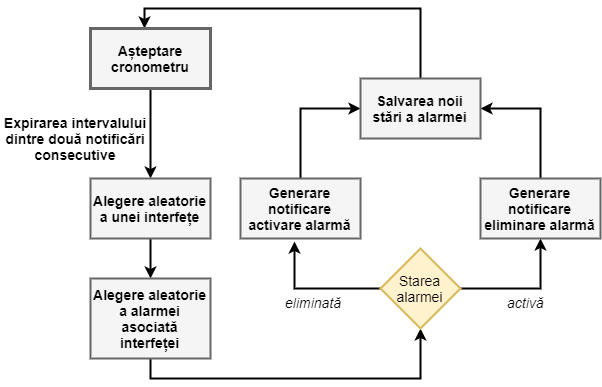
\includegraphics[width=1\textwidth]{wte_notif_generation}
	\caption{Organigrama mecanismului de generare a notificărilor NETCONF fictive al WTE.}
	\label{fig:wte_notif_generation}
\end{figure}

Până acum, generarea acestora se baza pe intervalul dintre două notificări consecutive definit în fişierul de configurare al \gls{dvm} și pe detaliile notificării ce se preluau din același loc. Acum, abordarea este diferită. În cazul notificărilor de tip \textit{valoarea atributului s-a schimbat - attributeValueChanged}, am modificat unealta care generează automat scheletul de cod C asociat serverului \gls{netconf}, astfel încât fiecare funcție cu apel invers asociată unui atribut configurabil va invoca funcţia ce trimite această notificare, conţinând valorile reale de care este nevoie: obiectul căruia i s-a schimbat valoare și noua valoare a acestuia. În acest mod, notificările de schimbare a valorii unui atribut nu mai sunt fictive, ci vor fi recepţionate de clienţii \gls{netconf} care s-au abonat la primirea acestora, chiar în momentul în care valoarea se schimbă. În cazul notificărilor de tip \textit{problemă - problemNotification}, sau alarmele pe care le generează dispozitivele de rețea, a fost păstrat principiul declanşării acestora în mod fictiv. Prin natura modelului informațional pentru microunde, fiecare interfață are asociată o listă de probleme pe care le poate avea și este definit și un număr minim de elemente pe care această listă să le aibă. \gls{wte} profită de acest aspect, implementând următorul mecanism de generare a alarmelor fictive: pentru fiecare problemă se retine starea acesteia: \textit{activă} sau \textit{eliminată}. Când intervalul dintre două notificări fictive consecutive s-a scurs, simulatorul se va pregăti să trimită o nouă notificare, astfel: se va alege în mod aleator o interfață a dispozitivului, iar din lista de probleme asociată interfeţei se va alege, din nou în mod aleator, o alarmă. În cazul în care starea acesteia este \textit{activă}, se trimite o notificare care conţine eliminarea acestei alarme și se schimbă starea asociată acestei probleme în \textit{eliminată}. Dacă starea acesteia era \textit{eliminată}, se va trimite o notificare care conţine activarea acestei probleme și starea ei va fi schimbată în \textit{activă}. Acest mecanism oferă dezvoltatorilor de aplicații \gls{sdn} un oarecare realism al simulatorului, alarmele fiind generate aleatoriu și, în cazul în care o alarmă era deja prezentă în echipamentul de control, există și posibilitatea ca această problemă să fie eliminată acum.

\subsection{Nucleul simulatorului WTE}

Nucleul simulatorului \gls{wte} reprezintă codul de bază ce oferă infrastructura care, împreună cu celelalte unelte software, furnizează funcţionalitatea propusă: emularea unei rețele de transport de date fără fir, în același timp expunând modelele informaționale dezvoltate de \gls{onf}, TR-532 și TR-512. Este implementat în limbajul Python, folosind o metodă orientată pe obiecte, fiind astfel flexibil și modular, oferind posibilitatea unei extinderi facile. Această abordare este similară cu cea folosită în cadrul celui mai important simulator pentru rețele definite prin software, \textit{mininet}. Asemănările, dar și motivele pentru care \gls{wte} nu a fost dezvoltat pe infrastructura oferită de \textit{mininet} vor fi detaliate în capitolul următor. Diagrama de clase a nucleului \gls{wte} este prezentată în Figura~\ref{fig:wte_class_diagram}.

\begin{figure}[h]
	\centering
	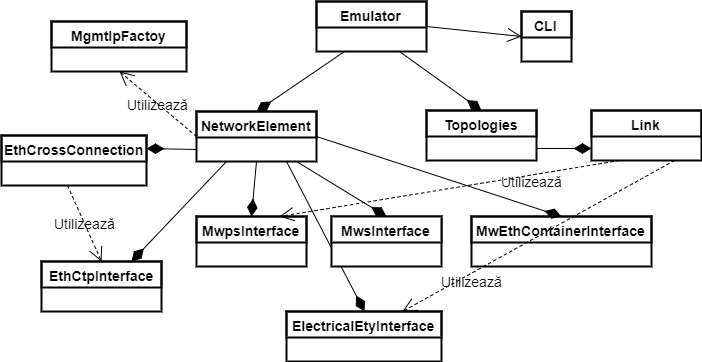
\includegraphics[width=1\textwidth]{wte_class_diagram}
	\caption{Diagrama de clase a nucleului WTE.}
	\label{fig:wte_class_diagram}
\end{figure}

Clasele proiectate pentru \gls{wte} sunt folosite în scopul reprezentării obiectelor care au o anumită semnificaţie în interiorul simulatorului. Astfel, clasa \textit{Emulator} este cea mai importantă, asigurând mediul în care toate celelalte instanţe ale obiectelor \gls{wte} vor fi create. Respectă modelul de programare obiect orientată \textit{Singleton}, însemnând că un singur obiect de acest tip va exista în momentul execuţiei programului. Este responsabilă de încărcarea și analizarea fişierelor \gls{json} de configurare a simulatorului. Parametrii din fişierul \textit{config.json} vor fi salvaţi ca variabile de execuţie, pentru a putea fi folosiţi ulterior. În cazul fişierului \textit{topology.json}, clasa \textit{Emulator} este responsabilă de analiza acestuia și de crearea obiectelor reprezentând elementele de rețea, respectiv legăturile de date dintre interfeţele acestora. Această clasă oferă și metode pentru executarea unor comenzi în maşina Linux sub care rulează \gls{wte}.

Clasa \textit{NetworkElement} este folosită pentru reprezentarea unui dispozitiv de rețea. În funcție de fişierul care descrie topologia, vor fi create mai multe instanţe ale acestei clase de către obiectul \textit{Emulator}. Atributele clasei sunt reprezentate, printre altele, de numele elementului de rețea, tipul acestuia (acest tip se referă de fapt la soluţia aleasă pentru implementarea serverului \gls{netconf} asociat, care poate fi \gls{dvm} sau altă variantă ce poate fi dezvoltată de către utilizator), lista conexiunilor Ethernet interne (reprezentând practic obiectele \gls{fc} din modelul informațional de bază), scheletul fişierului \gls{xml} care conţine atributele \gls{yang} configurabile, necesar pentru iniţializarea serverului \gls{netconf} și scheletul fişierului \gls{xml} care conţine atributele de stare, din care \gls{dvm} va returna valorile asociate acestora. Clasa \textit{NetworkElement} este responsabilă și pentru menținerea listei de obiecte reprezentând interfeţele pe care acel dispozitiv le prezintă. Oferă metode pentru crearea acestora, dar și pentru alterarea fişierelor \gls{xml} astfel încât să reflecte configurația definită de către utilizator în topologie. Celelalte metode importante pe care această clasă le oferă sunt în legătură cu lucrul cu containerul \textit{docker} asociat elementului de rețea: executarea de comenzi în interiorul containerul, iniţializarea containerului, copierea fişierelor \gls{xml} asociate \gls{dvm} în interiorul containerului \textit{docker}, etc.

Există mai multe clase care definesc obiecte de tip interfață a unui echipament de rețea, în funcție de tipul acestora. Tipul lor este dat de nivelul de transport specificat în modelul informațional de bază. Astfel, clasele asociate interfețelor de rețea sunt:
\begin{itemize}
	\item \textit{MwpsInterface} - asociată obiectelor \gls{ltp} de pe nivelul de transport \gls{mwps};
	\item \textit{MwsInterface} - asociată obiectelor \gls{ltp} de pe nivelul de transport \gls{mws};
	\item \textit{MwEthInterface} - asociată obiectelor \gls{ltp} de pe nivelul de transport \gls{etc};
	\item \textit{ElectricalEtyInterface} - asociată obiectelor \gls{ltp} de pe nivelul de transport \gls{ety};
	\item \textit{EthCtpInterface} - asociată obiectelor \gls{ltp} de pe nivelul de transport \gls{eth}.
\end{itemize}

Toate aceste clase oferă funcţionalitatea asociată unei interfețe, cu elementele specifice date de nivelul de transport la care operează (de exemplu relaţia client-server dintre obiectele \gls{ltp}, metode pentru alterarea fişierelor \gls{xml} asociate \gls{dvm} cu informații despre interfaţa respectivă, etc.).

Clasa \textit{Topology} reprezintă topologiile care se definesc în fişierul de configurare. Acestea pot fi prezente la două niveluri, \gls{mwps} și \gls{ety}. Aceste obiecte conţin de fapt obiectele de tip legătură, ce definesc topologia de rețea.

Clasa \textit{Link} reprezintă o legătură dintre două interfețe de rețea. Este responsabilă de stocarea celor două capete ce formează această legătură, dar și să valideze faptul că aceste capete sunt valide (există obiecte de tip interfață create anterior, între care se va putea face legătura efectivă). O metodă importantă pe care această clasă o oferă este cea responsabilă de crearea efectivă a legăturii (prin \gls{ovs} sau prin perechi Ethernet virtuale, așa cum va fi descris ulterior) dintre interfeţele de rețea Linux prezente în containerul \textit{docker}.

Figura~\ref{fig:wte_seq_diagram} prezintă o diagramă de secvenţă simplificată ce arată iniţializarea \gls{wte}.

\begin{figure}[h]
	\centering
	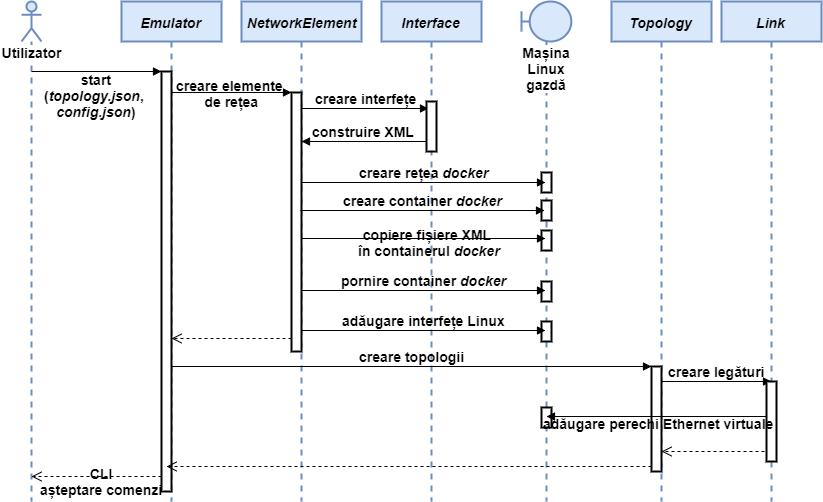
\includegraphics[width=1\textwidth]{wte_seq_diagram}
	\caption{Diagrama de secvenţă simplificată a inițializării WTE.}
	\label{fig:wte_seq_diagram}
\end{figure}

Construirea fişierelor \gls{xml} folosite de către \gls{dvm} este responsabilitatea fiecărui obiect dispozitiv de rețea, împreună cu interfeţele sale asociate. Fiecare obiect va altera modelul informațional adăugând informaţiile care îl reprezintă, astfel încât serverul \gls{netconf} să le pună la dispoziţie aplicațiilor \gls{sdn}. Apoi, aceste fişiere vor fi copiate în interiorul containerului \textit{docker} asociat și vor fi folosite de către \gls{dvm} pentru iniţializarea serverului \gls{netconf} și citirea valorilor atributelor de stare.

\subsection{Reprezentarea interfeţelor unui dispozitiv de rețea}

Fiecare interfață de rețea a echipamentelor, cu alte cuvinte fiecare obiect \gls{ltp} din modelul informațional de bază, indiferent de nivelul de transport pe care se află (\gls{mwps}, \gls{mws}, \gls{etc}, \gls{ety}, \gls{eth}), va fi reprezentată ca o interfață Linux, în interiorul containerului \textit{docker} asociat fiecărui dispozitiv de rețea. Legăturile interne din acest container, între interfeţele de rețea, vor fi descrise în paragrafele următoare. Pentru o mai bună înţelegere, acestea sunt prezentate în Figurile \ref{fig:wte_ltp_relationship} și \ref{fig:wte_ltp_ne_internal}.

\begin{figure}[h]
	\centering
	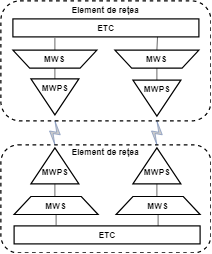
\includegraphics{wte_ltp_relationship}
	\caption{Obiectele LTP în contextul legăturii dintre două dispozitive de transport de date fără fir.}
	\label{fig:wte_ltp_relationship}
\end{figure}

\begin{figure}[h]
	\centering
	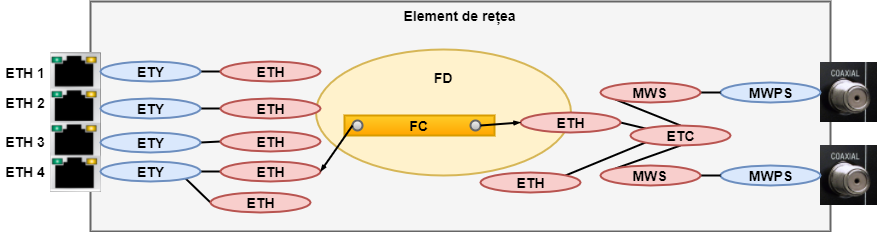
\includegraphics[width=1\textwidth]{wte_ltp_ne_internal}
	\caption{Obiectele LTP în interiorul unui dispozitiv de transport de date fără fir.}
	\label{fig:wte_ltp_ne_internal}
\end{figure}

Toate obiectele \gls{ltp} vor fi adăugate ca interfețe Linux având drept nume identificatorul unic universal asociat acestuia, așa cum este definit de către utilizator în fişierul de topologie al simulatorului. Adăugarea se va face cu ajutorul utilitarului \textit{\textbf{ip}}, oferit de Linux. Obiectele \gls{ltp} care se află la nivelurile \gls{mwps} sau \gls{ety} reprezintă interfețe ale dispozitivului de rețea cu exteriorul (radio, respectiv Ethernet). Astfel, dacă nu sunt definite legături în topologie care să utilizeze obiectul respectiv, acesta va fi reprezentat în containerul \textit{docker} drept o \textit{interfață fictivă de rețea (dummy interface)}. Adăugarea obiectului în Linux, în cazul în care acesta face parte dintr-o legătură va fi descrisă în sub-secţiunea următoare.

Obiectele \gls{ltp} de pe celelalte niveluri de transport vor avea, obligatoriu, o relaţie de tip client-server. Relaţiile, așa cum sunt definite în modelul informațional pentru microunde, sunt următoarele: obiectele de pe nivelurile \gls{mwps} și \gls{ety} nu își pot asuma rolul de client. Un obiect \gls{ltp} de pe nivelul \gls{mws} va avea drept server un obiect \gls{ltp} de pe nivelul \gls{mwps}, în timp ce un obiect \gls{ltp} de pe nivelul \gls{etc} va avea drept server un obiect \gls{ltp} de pe nivelul \gls{etc}. Obiectele \gls{ltp} de pe nivelul \gls{eth} pot avea ca server obiecte \gls{ltp} de pe nivelurile \gls{etc} sau \gls{ety}. Figura \ref{fig:wte_ltp_ne_internal} prezintă aceste legături. Soluția pentru reprezentarea acestor relaţii de tip client-server în Linux este folosirea interfeţelor de tip \textit{legătură (bond)}. O interfață de tip \textit{legătură} este o conexiune logică ce poate agrega mai multe interfețe. În acest mod, putem privi conexiunea logică, sau agregatorul, ca fiind clientul, iar interfeţele care sunt agregate ca fiind serverul. Considerând exemplul din Figura \ref{fig:wte_ltp_relationship}, pentru un element de rețea, obiectele \gls{ltp} de pe nivelul \gls{mws} vor fi reprezentate ca interfețe de tip \textit{legătură}, care agregă o singura interfață fiecare, dintre cele asociate obiectelor \gls{ltp} de pe nivelul \gls{mwps}, în timp ce obiectul \gls{ltp} de pe nivelul \gls{etc} va fi reprezentat printr-o interfață de tip \textit{legătură} ce va agrega cele două interfețe logice create pentru obiectele \gls{ltp} de pe nivelul \gls{mws}. Există mai multe moduri de funcţionare pentru interfeţele de tip \textit{legătură}, dar cel ales pentru \gls{wte} este acela în care distribuţia traficului pe conexiunile ce fac parte din acestă interfață logică este una simplă: conexiunile agregate sunt iterate și li se transmite câte un pachet de date, pe rând (\textit{round-robin}).

Obiectele \gls{ltp} de pe nivelul \gls{eth} sunt reprezentate ca interfețe virtuale de tip \textit{vlan}. Deoarece acestea au obligatoriu un identificator \gls{vlan} asociat, unei interfețe care reprezintă obiecte \gls{ltp} de pe nivelurile \gls{ety} sau \gls{etc} i se va putea asocia o interfață virtuală ce va semnifica obiectul \gls{ltp} de pe nivelul \gls{eth}.

Reprezentarea obiectelor de tip conexiuni Ethernet (\gls{fc}) este diferită față de celelalte. În acest caz, legătura dintre două obiecte de tip \gls{ltp} de pe nivelul \gls{eth} se face printr-o interfață logică de tip \textit{bridge}. Acesteia i se adaugă cele două interfețe de tip \textit{vlan} ce reprezintă cele două capete ale conexiunii Ethernet, astfel traficul va fi dirijat, prin interfaţa de tip \textit{bridge}, între acestea.

\subsection{Legăturile dintre interfeţele elementelor de rețea}

Au existat două abordări pentru reprezentarea legăturilor dintre elementele de rețea: prima metodă consta în realizarea unor conexiuni între două interfețe printr-un comutator software \gls{ovs}, iar cea de-a doua în crearea unei legături logice între două interfețe prin perechi Ethernet virtuale (\textit{veth pairs}). Cea din urmă a fost aleasă pentru implementare, însă vor fi prezentate ambele metode, pentru a înţelege de ce am făcut această alegere. Abordările considerate sunt ilustrate în Figura \ref{fig:wte_link_representation}.

\begin{figure}[h]
	\centering
	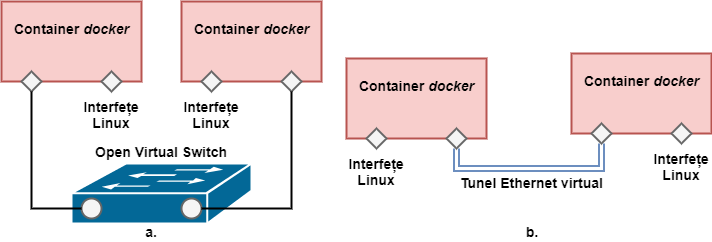
\includegraphics[width=1\textwidth]{wte_link_representation}
	\caption{Legăturile dintre interfeţele elementelor de rețea considerate pentru WTE: a) prin OVS; b) prin perechi Ethernet virtuale}
	\label{fig:wte_link_representation}
\end{figure}

Prima soluție considerată pentru reprezentarea legăturilor dintre interfeţele elementelor de rețea a fost prin intermediul unui comutator software \gls{ovs}. Astfel, pentru fiecare legătură trebuia creat un comutator \gls{ovs}, la care cele două capete ale legăturii (câte unul în fiecare container \textit{docker} asociat elementului de rețea) trebuiau legate. Ar fi fost posibilă și crearea unui singur comutator \gls{ovs} care să cuprindă toate legăturile din topologie, însă apoi trebuiau implementate restricţii la nivelul acestuia, pentru a nu exista legături nedorite (între alte interfețe decât cele specificate în fişierul de topologie). Modelarea legăturii fără fir era posibilă prin aplicarea unor restricţii de calitate de servicii - \gls{qos} asupra conexiunii respective, în interiorul comutatorului \gls{ovs} (de exemplu lărgimea de bandă să fie una specifică unei legături între echipamente de transport de date fără fir). Această abordare prezenta însă un dezavantaj major. Presupunând că o interfață Linux dintr-un container \textit{docker} ar fi fost dezactivată, era de așteptat ca acest lucru să fie vizibil și în celălalt capăt al legăturii și interfaţa îndepărtată să raporteze o stare operaţională \textit{închisă}. Deoarece legătura era făcută prin comutatorul software \gls{ovs}, acest lucru nu s-ar fi întâmplat, pentru că stările porturilor din comutator sunt independente și nu s-ar fi propagat între porturile prin care se face conexiunea. Acest dezavantaj major a condus la căutarea unei alte soluții pentru reprezentarea acestor legături. O altă problemă pe care această abordare o ridică este consumul de resurse. Fiecare legătură va avea propriul comutator \gls{ovs} asociat, astfel că pentru o topologie de rețea cu multe conexiuni, va exista un consum de resurse nejustificat de mare. De asemenea, instalarea \gls{wte} pe maşina Linux gazdă va fi mai greoaie, deoarece ar implica și instalarea prealabilă a \gls{ovs}.

Răspunsul la provocările menţionate anterior constă în următorul concept pus la dispoziţie de Linux: perechi Ethernet virtuale. Acestea reprezintă perechi de interfețe virtuale Linux de rețea care sunt conectate printr-un \textit{tunel}. Tot traficul care va intra într-o interfață va fi dirijat către interfaţa pereche, ca și când acestea ar fi conectate printr-un cablu Ethernet virtual. În cazul \gls{wte}, în momentul în care se încearcă reprezentarea unei legături din fişierul de topologie, o astfel de pereche este creată. Apoi, un capăt al conexiunii va fi asociat containerului \textit{docker} asociat primului dispozitiv de rețea al legăturii, iar celălalt capăt celui de-al doilea container \textit{docker}. În acest mod, în momentul în care una dintre interfețe este dezactivată, acest lucru se va propaga imediat la interfaţa îndepărtată, care va raporta o stare operaţională \textit{închisă}. Modelarea unei legături fără fir se poate face în mod facil folosind această abordare. Linux oferă utilitarul \textit{\textbf{tc}} - Traffic Control. Acesta poate instrui nucleul sistemului de operare să altereze caracteristicile unei interfețe virtuale, precum: debitul interfeţei, latenţa pe care interfaţa o introduce în traficul pe care îl transportă, procentul de pachete pe care interfaţa de poate pierde, etc.

Pe baza considerentelor expuse anterior, a fost implementată ce-a de-a doua soluție pentru reprezentarea legăturilor dintre interfeţele echipamentelor de rețea: folosirea perechilor Ethernet virtuale.

\subsection{Modelarea conexiunilor dintre dispozitivele simulate ca legături fără fir}

O parte importantă a \gls{wte}, care este reprezentativă pentru considerarea acestuia ca fiind un simulator de rețele de transport de date fără fir, nu doar o unealtă care expune modelele informaționale dezvoltate de \gls{onf} conform cu fişierul în care este definită topologia, este dată de modelarea conexiunilor dintre dispozitivele de rețea simulate având caracteristicile unei legături fără fir.

Caracteristicile ce pot fi alterate prin unealta \textit{\textbf{tc}} oferită de Linux, care sunt relevante pentru simularea unei legături fără fir, sunt reprezentate de debitul interfeţei, întârzierea pachetelor ce tranzitează această conexiune și procentul de pachete pierdute.

Debitul unei interfețe este influenţat de mai mulți parametri, dintre care unii sunt configurabili. TR-532 oferă și o formulă de calcul pentru acest debit, tocmai pentru ca aplicațiile \gls{sdn} ce se folosesc de acest model să fie aliniate asupra acestei metode. Ecuația \ref{eq:txCapacityFormula} descrie această metodă de calcul.

\begin{equation}\label{eq:txCapacityFormula}
\begin{split}
txCapacity& =AirInterface::AirInterfaceConfiguration::\textbf{\textit{txChannelBandwidth}}\\
& \quad * \log_{2}(AirInterface::AirInterfaceStatus::\textbf{\textit{modulationCur}})\\
& \quad * AirInterface::AirInterfaceStatus::\textbf{\textit{codeRateCur}} * 0,85
\end{split}
\end{equation}
unde:

$txCapacity$ = debitul interfeţei de rețea, în kbps

$txChannelBandwidth$ = lărgimea de bandă a emiţătorului, în kHz

$modulationCur$ = schema de modulaţie folosită, în număr de simboluri

$codeRateCur$ = procentul informaţiei utile din informaţia transmisă\\

Rata de transmisie a încărcăturii utile, reprezintă produsul dintre rata de transmisie brută și procentul informaţiei utile din informaţia transmisă ($codeRateCur$), unde acesta reprezintă numărul de biţi ai încărcăturii utile, raportat la numărul total de biţi transmişi. Acest procent apare din cauza redundanţei introduse pentru corectarea de erori și alte informații care nu fac parte din încărcătura utilă și are o valoare tipică între 0,85 și 0,95~\cite{kizer2013digital}. În cazul \gls{wte}, am considerat valoarea acestei rate curente a codului ca fiind 0,9.

Rata de transmisie brută este definită ca produsul dintre rata simbolurilor și numărul de biţi per simbol. Valoarea acestuia din urmă este dată de modulaţia folosită la transmisie. Modulaţia tipică folosită în echipamentele de transport de date fără fir este Modulaţia de Amplitudine în Cuadratură - \gls{qam}. În acest caz, numărul de biţi per simbol este definit ca $\log_{2}$ din numărul de constelaţii (reprezentat în modelul informațional prin $modulationCur$). Rata simbolurilor tipică pentru acest tip de echipamente este de aproximativ 85\% din lărgimea de bandă ($txChannelBandwidth$) a canalului de transmisie~\cite{kizer2013digital}.

Această formulă este implementată în cadrul \gls{wte}. În momentul în care unul dintre atributele unei interfețe pe baza cărora se face calculul se schimbă (de exemplu o aplicație \gls{sdn} modifică lărgimea de bandă folosită de o interfață a unui echipament, sau modulaţia care se folosește pentru transmisie), instanţa \gls{dvm} asociată dispozitivului de rețea va calcula debitul interfeţei respective și apoi va folosi utilitarul Linux \textit{\textbf{tc}} pentru a modifica această caracteristică a interfeţei. În acest mod, legăturile fără fir vor fi modelate în simulator astfel încât să semene cu cele din rețelele reale, din punctul de vedere al ratei de transmisie.

În legătură cu latenţa pe care o introduc echipamentele de transport de date fără fir, tipic aceasta este de ordinul zecilor sau sutelor de microsecunde~\cite{kizer2013digital}. Această plajă de întârzieri nu pot fi simulate în cadrul \gls{wte}, deoarece utilitarul \textit{\textbf{tc}} oferă modificarea latenţei unei interfețe de rețea doar cu o rezoluţie de o milisecundă. Pentru a putea beneficia de rezoluţii mai mici, de ordinul microsecundelor, imaginea sistemului de operare Linux din containerul \textit{docker} ar trebui modificată și nucleul sistemului de operare recompilat, astfel încât să permită utilizarea unor cronometre de sistem de timp real. Versiunea curentă a \gls{wte} nu implementează acest comportament, dar acesta poate constitui subiectul unei alte cercetări, pentru a modela legăturile dintre interfeţele dispozitivelor de rețea simulate cât mai aproape de realitate.

Alterarea procentului de pachete pierdute de o interfață de rețea nu este încă folosit în \gls{wte}, deoarece presupunem că legătura fără fir este realizată în condiţii atmosferice optime, astfel încât să nu se piardă pachete. Ar putea fi totuşi utilizat, spre exemplu prin expunerea unei comenzi în linia de comandă a simulatorului, care să crească sau să scadă acest procent pentru o conexiune. Astfel, s-ar putea simula condiţii atmosferice potrivnice în anumite părţi ale topologiei de rețea. În acest mod ar putea fi testată, de exemplu, o aplicație \gls{sdn} care să detecteze faptul că există probleme în rețea (din cauza unei furtuni se pierd pachete, sau scade modulaţia folosită la emisie) și să dirijeze traficul prin altă parte a topologiei.

\subsection{Linia de comandă}

\gls{wte} dispune de un modul care oferă o interfață prin linie de comandă utilizatorului. După ce acesta porneşte simulatorul, la sfârşitul inițializării (adică după ce au fost create toate obiectele asociate cu topologia de rețea specificată în fişierul de configurare) se lansează modulul care implementează interfaţa prin linie de comandă - \gls{cli}. Acesta oferă utilizatorului posibilitatea unei interacţiuni simple cu simulatorul, prin furnizarea unor comenzi clare, simplu de folosit. O captură de ecran a acestei interfețe este prezentată în Figura \ref{fig:wte_cli_screenshot}.

\begin{figure}[h]
	\centering
	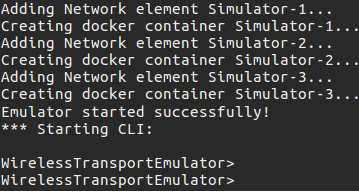
\includegraphics{wte_cli_screenshot}
	\caption{Captură de ecran a interfeţei prin linie de comandă a WTE.}
	\label{fig:wte_cli_screenshot}
\end{figure}

Comenzile implementate sunt următoarele:
\begin{itemize}
	\item \textit{afişare noduri} - afişează pe ecran numele tuturor dispozitivelor de rețea simulate;
	\item \textit{afişare informații nod} - afişează pe ecran toate informaţiile disponibile despre un anumit echipament de rețea simulat: nume, adresa \gls{ip} a interfeţei de administrare, portul folosit de serverul \gls{netconf}, lista interfeţelor nodului respectiv împreună cu nivelul de transport pe care acesta se află;
	\item \textit{afişare legături} - afişează pe ecran toate legăturile dintre interfețe prezente în topologia simulată, inclusiv nivelul de transport la care este realizată aceasta (\gls{mwps} sau \gls{ety});
	\item \textit{pornire terminal} - porneşte un terminal care se leagă la containerul \textit{docker} asociat unui element de rețea, oferind acces la mediul Linux din interiorul imaginii. Acesta poate fi folosit de utilizator pentru a interacţiona într-un mod facil și direct cu elementul de rețea respectiv.
	\item \textit{înregistrare / anularea înregistrării \gls{odl}} - această comandă oferă posibilitatea de a înregistra / anula înregistrarea în mod automat pentru elementele de rețea la / de la echipamentul de control \gls{sdn} (în particular \gls{odl}). Detaliile de conectare la echipamentul de control \gls{sdn} sunt cele specificate în fişierul de configurare al \gls{wte};
	\item \textit{închidere} - această comandă poate fi folosită de către utilizator pentru închiderea simulatorului (împreună cu toate obiectele pe care acesta le-a creat în interiorul maşinii Linux gazdă).
\end{itemize}

\subsection{Generarea traficului de date}

Pentru a oferi o soluție completă de simulare, inclusiv validarea topologiei și a legăturilor create, \gls{wte} pune la dispoziţie utilizatorilor și posibilitatea de a genera trafic de date între anumite puncte ale rețelei. În acest scop este folosită unealta software \textit{iperf3} \cite{iperf32017, tirumala2005iperf}. Aceasta este instalată în sistemul de operare Linux din imaginea \textit{docker} folosită de fiecare dispozitiv de rețea simulat.

Toate conexiunile descrise până acum sunt făcute la nivelul 2 (legătură de date) din stiva \gls{osi}. Astfel, interfeţele Linux din containerul \textit{docker} nu folosesc adrese \gls{ip} (în afară de cea de administrare). Generarea de trafic se face între două interfețe, una jucând rolul de client, iar cealaltă de server. Pentru ca unealta \textit{iperf3} să poată funcţiona, este nevoie de adăugarea de adrese \gls{ip} celor două interfețe. \gls{wte} poate face acest lucru în mod automat, dacă în fişierul care descrie topologia, obiectului \textit{conexiune Ethernet} i se adaugă un atribut \textit{gazdă}. Astfel, acelui obiect i se asociază, la nivel teoretic, un port capabil să genereze sau să recepţioneze trafic. Practic, o adresă \gls{ip} este adăugată la interfaţa asociata acelui obiect. Apoi, utilizatorul va putea genera trafic între oricare două astfel de porturi. 

Unealta \textit{iperf3} permite generarea de trafic \gls{tcp} sau \gls{udp}, oferind în același timp posibilitatea de a măsura latenţa pachetelor, variaţia acestei latenţe (jitter) sau lărgimea de bandă a canalului de comunicaţie folosit.
\section{Folosirea în contextul demonstraţiilor de concept}

Primele două versiuni ale \gls{dvm} au fost unelte foarte importante pentru cea de-a doua și cea de-a treia demonstraţie de concept desfăşurate în cadrul \gls{onf}. În același mod, \gls{wte} a fost o unealtă critică în contextul celei de-a patra demonstraţii de concept a proiectului \gls{wt} din grupul \gls{otwg}, care a dus la accelerarea și o bună desfăşurare a acesteia. A permis dezvoltatorilor de aplicații \gls{sdn} testarea unor implementări mai avansate, ce nu puteau fi acoperite de simulatoarele precedente, prin oferirea unei modalităţi facile de a simula diferite topologii de rețea, prin simpla descriere a acestora într-un fişier.

Pe lângă expunerea modelelor informaționale TR-532 și TR-512.1, \gls{wte} permite și modelarea legăturilor fără fir dintre dispozitivele de rețea simulate. Astfel, se pot testa și aplicații care influenţează dirijarea traficului în rețea. O versiune ulterioară a \gls{wte} va permite chiar simularea unor evenimente care influenţează traficul de date (de exemplu atenuări introduse pe o legătură fără fir de vreme nefavorabilă).

Un alt avantaj față de versiunile anterioare, care a fost folosit în cea de-a patra demonstraţie de concept, a constat în expunerea a încă două modele informaționale, care încă nu au fost lansate oficial de către \gls{onf}: un model informațional pentru Ethernet și un model informațional pentru sincronizare, bazat pe \gls{ptp}.

Modelul informațional pentru Ethernet a fost unul simplificat, având aceeaşi structură ca elemente ce se găsesc în modelul informațional pentru microunde: capabilităţi, configuraţie, stare, problemele curente, valori de performanţă curente și valori de performanţă istorice, legătura cu modelul de bază făcându-se printr-un obiect \gls{lp}. Singurul parametru configurabil în acest model simplificat a fost identificatorul rețelei locale virtuale (\gls{vlan} ID). Acest model reprezintă pachetul condiţional asociat obiectelor \gls{ltp} de pe nivelul de transport \gls{eth}. Identificatorul rețelei locale virtuale a fost reprezentat ca parametru al interfeţelor virtuale de tip \textit{vlan}, în interiorul containerelor \textit{docker}.

Modelul pentru sincronizare a fost o extindere a modelului dezvoltat de \gls{itu-t} pentru protocolul \gls{ptp}. Extinderea a constat în adăugarea unor parametri, dar și integrarea cu modelul informațional de bază, printr-un obiect \gls{lp}. Parametrii asociaţi acestui model nu au avut echivalent în implementarea interfeţelor în sistemul de operare Linux al containerelor \textit{docker}, au avut doar valori implicite ce au fost expuse echipamentului de control \gls{sdn}.

\subsection{Implementare alternativă de server NETCONF}

Arhitectura modulară și abordarea flexibilă pe care se bazează \gls{wte} facilitează integrarea acestuia cu alte implementări de servere \gls{netconf}, în funcție de nevoile fiecărui utilizator. În acest scop, trebuie folosită aceeași abordare, în sensul în care implementarea de server dorită trebuie să ofere un container \textit{docker} care să poată fi utilizat de către infrastructura \gls{wte}, pentru simularea elementelor de rețea.

În contextul celei de-a patra demonstraţii de concept \gls{onf}, o companie membră a proiectului \gls{wt}, \textit{highstreet technologies} a ales să integreze propriul server \gls{netconf}, o implementare Java bazată tot pe fişiere de configurare \gls{xml}, dar cu mult mai puţine facilități decât \gls{dvm}. Au făcut această alegere deoarece implementarea lor era potrivită doar pentru teste simple și rapide, oferind o soluție de server \gls{netconf} mai uşor de folosit decât \gls{dvm}.

Chiar dacă au renunţat la facilităţile oferite de \gls{wte} în combinație cu \gls{dvm} (precum simularea legăturilor fără fir), soluţia lor a demonstrat utilitatea infrastructurii folosite de simulator și faptul ca aceasta poate fi extinsă într-un mod facil, pentru a îndeplini și alte nevoi ale utilizatorilor. Practic, faptul că \gls{wte} a fost folosit de unul dintre membrii proiectului și pentru altceva în afară de utilizarea obişnuită (adică doar rularea simulatorului, cu scopul testării unor aplicații \gls{sdn}), mai exact pentru extinderea acestuia prin integrarea cu altă soluție de server \gls{netconf}, a validat încă o dată, soluţia \gls{wte}.

Chiar dacă cea de-a patra demonstraţie de concept \gls{onf} s-a terminat, \gls{wte} oferă în continuare posibilitatea executării cazurilor de utilizare propuse și chiar dezvoltarea de noi aplicații care să folosească modelele informaționale propuse de \gls{onf} (de bază, pentru microunde, pentru Ethernet și pentru sincronizare). În acest scop, mediul de simulare pus la dispoziţie de \gls{wte} a fost instalat și încă rulează, până la sfârşitul anului 2017, într-un mediu \textit{Cloud} asigurat de gazda celei de-a patra demonstraţii de concept, \textit{Deutsche Telekom}. Utilizatorilor interesaţi li se poate oferi acces la acel mediu de simulare și la echipamentul de control \gls{sdn}, pentru a putea vizualiza cazurile de utilizare propuse, sau pentru a dezvolta altele.

\chapter{Rezultate și discuţii\label{ch:rezultate_discutii}}

\section{Evaluarea WTE}

Pentru a evalua simulatorul propus în această lucrare, au fost considerate patru caracteristici pentru a fi măsurate: puterea de procesare pe care simulatorul o folosește, procentul de \textit{memorie cu acces aleator} - \gls{ram} necesar funcţionării acestuia, timpul de iniţializare a simulatorului și spaţiul de stocare ocupat pe disc de \gls{wte}. Metoda de măsurare a acestor caracteristici și rezultatele acestora vor fi prezentate în paragrafele următoare.

\subsection{Metodologie}

Pentru a putea măsura cele patru caracteristici menţionate anterior, a fost nevoie de dezvoltarea unor soluții în simulator. Acestea au fost implementate în nucleul \gls{wte}.

Măsurarea timpului de iniţializare a simulatorului, a constat în folosirea unui cronometru oferit de limbajul Python. Acesta a fost pornit după citirea fişierelor de configurare și oprit după ce toate elementele topologiei simulate au fost create, înainte de pornirea interfeţei prin linie de comandă. Timpul astfel măsurat reprezintă durata de iniţializare a simulatorului și este exprimat în secunde, cu o precizie de trei zecimale. Valoarea acestuia a fost tipărită în consola simulatorului.

O abordare similară a fost folosită și în determinarea spațiului de stocare pe disc folosit de \gls{wte}. Înainte de începerea inițializării simulatorului se interoghează sistemul de operare asupra spațiului liber de pe disc. După terminarea inițializării se face o nouă interogare, diferenţa dintre aceste două valori reprezentând spaţiul pe disc ocupat de topologia simulată. Este ocupat și spațiu pe disc, nu doar în memoria \gls{ram} din cauza abordării folosite în utilitarul \textit{docker}, în care fiecare container are nevoie de spațiu pentru a-și reprezenta sistemul de fişiere din interior. Valoarea calculată este exprimată în MB și este afişată de asemenea în consola simulatorului, după terminarea inițializării.

Procentul memoriei cu acces aleator utilizat de simulator este dat, în cea mai mare parte, de către memoria necesară containerelor \textit{docker} asociate fiecărui element de rețea. Nucleul \gls{wte}, în calcularea acestui procent, neglijează alte valori (de exemplu chiar acest nucleu folosește la rândul său memorie cu acces aleator, care nu este însă semnificativă în comparaţie cu celelalte valori) și se bazează
doar pe valorile asociate containerelor \textit{docker}. În interfaţa prin linie de comandă a simulatorului a fost implementată o comandă care să calculeze acest procent. Calculul folosește informaţiile furnizate de o comandă a utilitarului \textit{docker}: \textit{docker stats}. Aceasta afişează procentul de memorie cu acces aleator utilizat de fiecare container care rulează. Implementarea comenzii din nucleul \gls{wte} va aduna aceste valori și va afişa pe ecran suma. Valoarea tipărită pe ecran reprezintă procentul de memorie cu acces aleator folosit pentru simularea topologiei de rețea.

Calcularea puterii de procesare a \gls{wte} se face prin aceeaşi comandă care afişează și procentul de memorie cu acces aleator folosit. Implementarea acesteia utilizează, de asemenea, comanda \textit{docker stats} oferită de utilitarul \textit{docker}, însă abordarea este puţin diferită. Diferenţa este dată de faptul că puterea de procesare nu este folosită în mod continuu de către containerele \textit{docker} asociate elementelor de rețea simulate. Astfel, dacă în momentul interogării sistemului de operare, unor containere nu le erau alocate cuante de timp de procesare, acestea apar cu zero procent de utilizare a procesorului. La o interogare ulterioară, acest procent ar putea fi altfel distribuit dispozitivelor simulate. Pentru ca valoarea măsurată să fie relevantă, a fost ales un număr de zece eşantioane pentru fiecare element de rețea simulat, procentul de putere de procesare asociat fiind reprezentat de media aritmetică a acestora. În mod empiric a fost observat că dacă s-ar fi ales un număr mai mare de eşantioane, de exemplu o sută, diferenţa valorii procentului final calculat ar fi fost foarte mică față de cazul celor zece eşantioane. Astfel, pentru a nu prelungi inutil timpul de calcul al acestui procent, s-a rămas la abordarea cu zece eşantioane. De asemenea, acest procent al puterii de procesare oferit de comanda \textit{docker stats} este raportat la un singur nucleu al procesorului, astfel încât în condiţii de utilizare intensă am fi putut avea valori ale procentului mai mari de 100\%. Din acest motiv, valoarea procentuală raportată a fost împărţită la numărul de nuclee ale procesorului. Pe scurt, procentul puterii de procesare se calculează astfel: se interoghează sistemul de operare prin comanda \textit{docker stats} asupra procentului folosit de fiecare container în parte și se face suma acestora. Acest lucru se repetă de zece ori (numărul de eşantioane considerat) și apoi se face media aritmetică. Valoarea astfel obţinută se împarte la numărul de nuclee ale procesorului, obţinând astfel valoarea finală a procentului de putere de procesare utilizată de simularea topologiei de rețea, care este afişată pe ecran.

Puterea de procesare și procentul de memorie cu acces aleator utilizate de către \gls{wte} au fost măsurate doar după ce dispozitivele simulate au fost înregistrate la echipamentul de control \gls{sdn}, stabilindu-se astfel conexiunile \gls{netconf} din rețea.

Toţi parametrii care au fost menţionaţi anterior au fost măsuraţi în diferite topologii tipice pentru rețelele de transport de date fără fir: topologii de tip inel (\textit{ring}), de tip arbore (\textit{tree}) sau de tip plasă (\textit{mesh}). Exemple de astfel de topologii, împreună cu detaliile dispozitivelor de rețea simulate în fiecare caz sunt ilustrate în Figurile~\ref{fig:topologies_ring}, \ref{fig:topologies_tree} și \ref{fig:topologies_mesh}.

\begin{figure}[h]
	\centering
	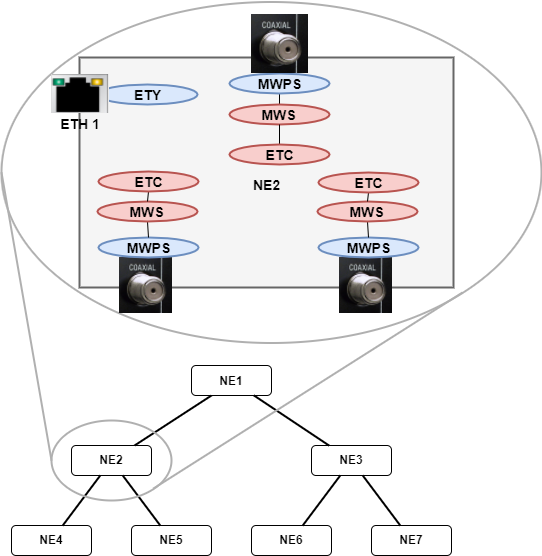
\includegraphics[width=0.6\textwidth]{topologies_tree}
	\caption{Topologie de rețea arbore, exemplu pentru 7 elemente simulate}
	\label{fig:topologies_tree}
\end{figure}

\begin{figure}[h]
	\centering
	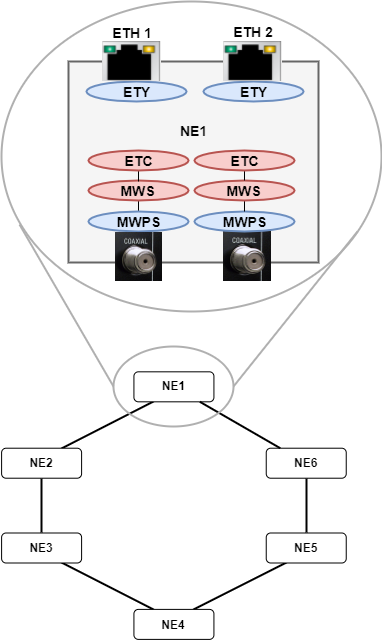
\includegraphics[width=0.6\textwidth]{topologies_ring}
	\caption{Topologie de rețea inel, exemplu pentru 6 elemente simulate}
	\label{fig:topologies_ring}
\end{figure}

\begin{figure}[h]
	\centering
	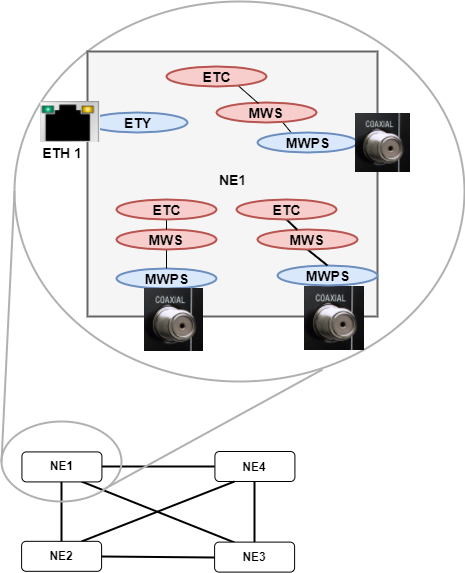
\includegraphics[width=0.6\textwidth]{topologies_mesh}
	\caption{Topologie de rețea plasă, exemplu pentru 4 elemente simulate}
	\label{fig:topologies_mesh}
\end{figure}

În cazul rețelelor de tip inel, au fost simulate topologii având un număr de elemente simulate de la 10 la 200, acesta crescând din 10 în 10. În această situaţie, un dispozitiv simulat are nevoie de două interfețe fără fir, reprezentate în modelele propuse de \gls{onf} prin obiecte de tip \gls{mwps}, pentru conexiunile cu vecinii. Fiecare astfel de interfață va avea și obiecte de tip \gls{mws} și \gls{etc} asociate. A fost aleasă și asocierea a două interfețe Ethernet fiecărui dispozitiv simulat, pentru a putea injecta trafic în nodul respectiv, reprezentată de obiecte de tip \gls{ety}. Astfel, fiecare dispozitiv simulat prezintă un număr de opt obiecte, care sunt reprezentate în containerul \textit{docker} asociat prin opt interfețe Linux.

Topologiile de tip arbore alese pentru simulare în cadrul evaluării au fost reprezentate de arbori binari. În acest caz, fiecare dispozitiv de rețea a avut nevoie de trei interfețe fără fir (una pentru conexiunea dinspre rădăcină și două pentru legăturile dinspre frunze), reprezentate prin obiecte de tip \gls{mwps}. Fiecare astfel de interfețe au asociate și obiectele de tip \gls{mws} și \gls{etc}. Fiecare element de rețea simulat a avut asociată și o interfață de tip Ethernet prin care să se poată injecta trafic, reprezentată de un element de tip \gls{ety}. În acest mod fiecare container \textit{docker} asociat a avut nevoie de zece interfețe Linux pentru reprezentarea internă a acestor obiecte. În simulările asociate evaluării au fost folosite topologii în care a fost variată adâncimea arborelui, de la 3 (însemnând un număr de 7 elemente de rețea), până la 7 (127 de dispozitive simulate).

Topologiile de tip plasă cu redundanţă maximă diferă de celelalte prin faptul că numărul total de interfețe simulate nu mai creşte liniar, ca în cazurile anterioare, ci pătratic cu numărul de elemente de rețea. Pentru o topologie de tip plasă cu $ N $ elemente de rețea vom avea un număr total de interfețe simulate de $ N(N-1) $ și respectiv $ N(N-1)/2 $ legături de date. Astfel, pentru \textit{N} elemente, fiecare dispozitiv simulat prezintă \textit{N-1} obiecte de tip \gls{mwps} pentru conexiunile dintre echipamente, respectiv \textit{N-1} obiecte de tip \gls{mws} și \textit{N-1} obiecte \gls{etc}. Fiecare astfel de dispozitiv are asociată și o interfață Ethernet (un obiect \gls{ety}), pentru injectarea de trafic.

Măsurătorile pentru evaluare au fost efectuate în trei medii diferite în care a fost instalat simulatorul \gls{wte}: local, pe un laptop cu o mașină virtuală Linux și în două medii de tip \textit{cloud}. Primul mediu \textit{cloud}, denumit Orbit \cite{orbitpage}, a fost pus la dispoziţie de compania AT\&T. Cel de-al doilea mediu este cel folosit în cea de-a patra demonstraţie de concept \gls{onf} și a fost asigurat de Deutsche Telekom (DT). Caracteristicile, precum și resursele de care dispune fiecare dintre aceste mașini sunt reprezentate în Tabelul~\ref{tab:resources}.

\begin{table}[h]
	
	\caption{Caracteristicile maşinilor pe care s-a făcut evaluarea WTE.\label{tab:resources}}
	\begin{tabular}{|M{0.25\textwidth}|M{0.2\textwidth}|M{0.2\textwidth}|M{0.2\textwidth}|}
		\hline
		\textbf{Caracteristica} & \textbf{\emph{Mașina locală}} & \textbf{\emph{Orbit Cloud}} & \textbf{\emph{DT Cloud}} \tabularnewline
		\hline 
		Sistemul de operare & Linux & Linux & Linux \tabularnewline
		\hline 
		Versiunea de kernel & 4.4.0-93-generic & 4.4.0-83-generic & 4.4.0-89-generic
		\tabularnewline
		\hline 
		Arhitectura procesorului & x86\_64 & x86\_64 & x86\_64 \tabularnewline
		\hline 
		Memoria cu acces aleator & 4096 MB & 8 GB & 8GB \tabularnewline
		\hline 
		Capacitatea de stocare a discului & 32 GB & 80 GB & 80 GB \tabularnewline
		\hline 
		Frecvenţa procesorului & 2591.59 MHz & 2 GHz & 2500 MHz \tabularnewline
		\hline 
		Nuclee procesor & 4 & 4 & 4 \tabularnewline
		\hline \end{tabular}
\end{table}

%\subsection{Rezultatele măsurătorilor}

\subsection{Timpul de inițializare a simulatorului}

Prima caracteristică măsurată în procesul de evaluare a fost timpul de iniţializare a simulatorului. Acesta reprezintă durata de când simulatorul \gls{wte} este pornit, până când toate elementele rețelei (dispozitive, interfețe ale acestora și legăturile dintre ele) au fost adăugate în mediul de simulare și interfaţa prin linie de comandă este accesibilă. Figura~\ref{fig:boot_vs_ne_ring_v1} prezintă variaţia timpului de iniţializare cu numărul de elemente de rețea simulate, în cazul unei topologii de tip inel. Din cauza faptului că maşina locală are doar 4 GB de memorie cu acces aleator, simularea în acest mediu se opreşte la 130 de dispozitive simulate. În Figura~\ref{fig:boot_vs_ne_tree_v1} este ilustrată aceeaşi variaţie, în cazul simulării unei topologii de tip arbore, în timp ce Figura~\ref{fig:boot_vs_ne_mesh_v1} este folosită pentru a descrie cazul topologiei de tip plasă. Acestea arată o dependenţă liniară (aproximativ) între numărul de dispozitive simulate și timpul de iniţializare. 

\begin{figure}[hp]
	\centering
	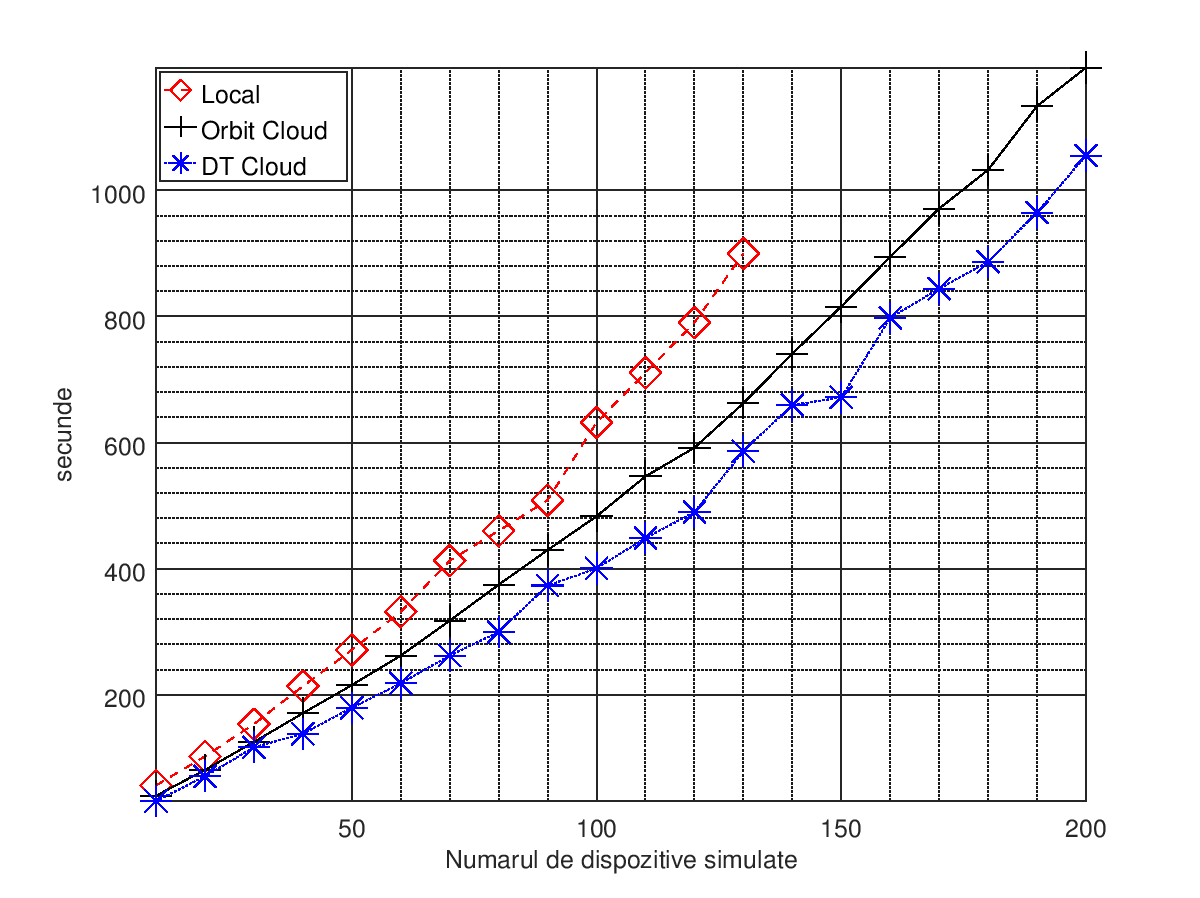
\includegraphics[width=0.85\textwidth]{boot_vs_ne_ring_v1}
	\caption{Timpul de iniţializare în funcție de numărul de dispozitive de rețea simulate, într-o rețea de tip \textbf{inel}}
	\label{fig:boot_vs_ne_ring_v1}
\end{figure}

\begin{figure}[hp]
	\centering
	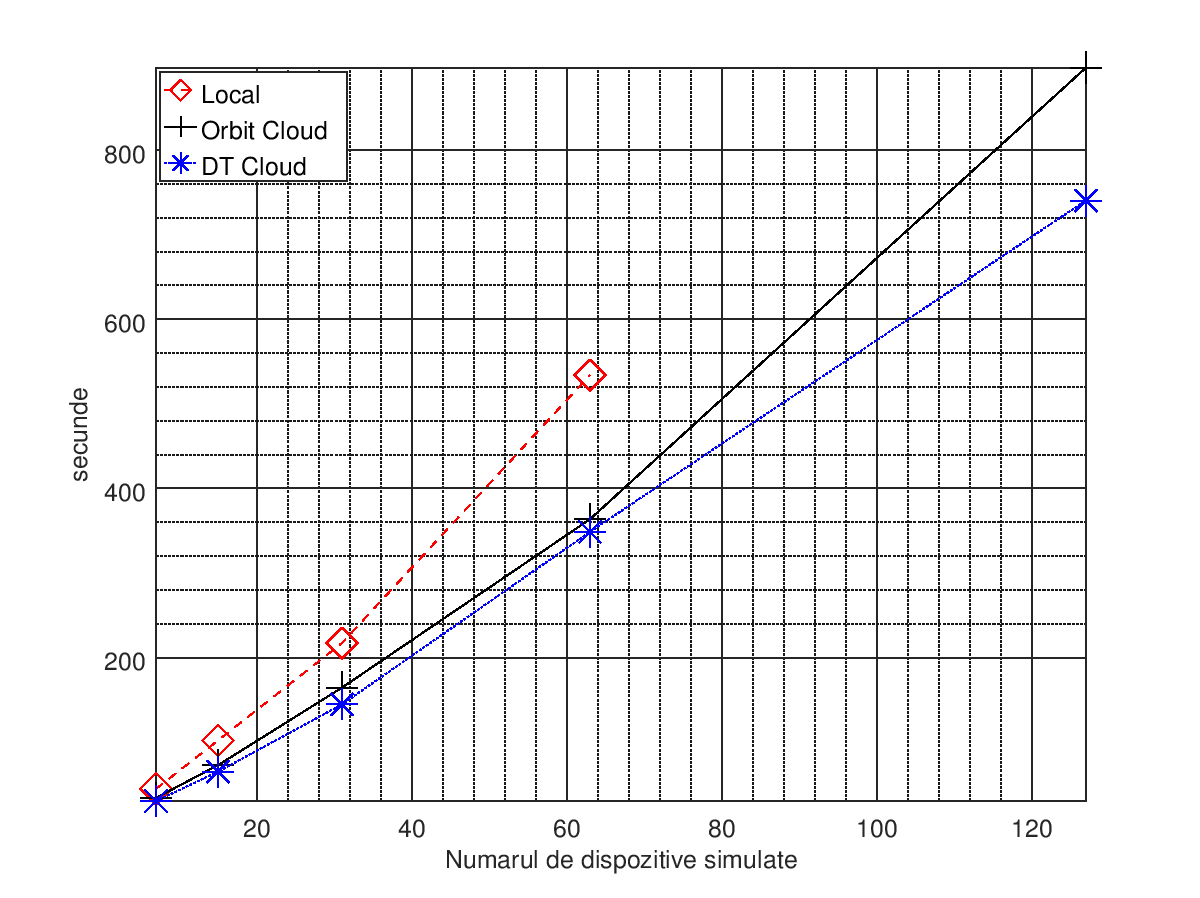
\includegraphics[width=0.85\textwidth]{boot_vs_ne_tree_v1}
	\caption{Timpul de iniţializare în funcție de numărul de dispozitive de rețea simulate, într-o rețea de tip \textbf{arbore}}
	\label{fig:boot_vs_ne_tree_v1}
\end{figure}

\begin{figure}[hp]
	\centering
	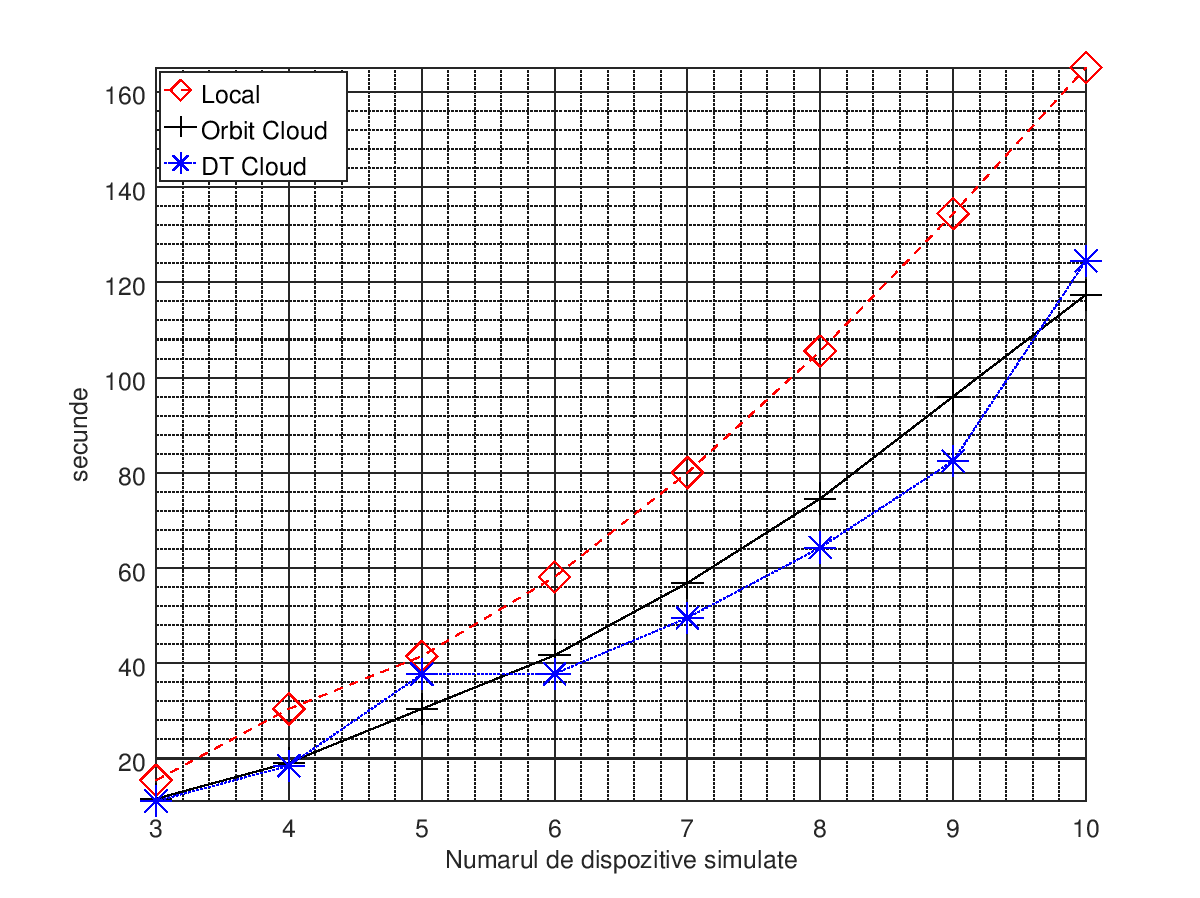
\includegraphics[width=0.85\textwidth]{boot_vs_ne_mesh_v1}
	\caption{Timpul de iniţializare în funcție de numărul de dispozitive de rețea simulate, într-o rețea de tip \textbf{plasă}}
	\label{fig:boot_vs_ne_mesh_v1}
\end{figure}

Se poate observa că, deşi frecvenţa procesorului în cazul măsurătorilor locale este mai mare decât cea a procesoarelor din mediile de tip \textit{cloud}, din cauza faptului că există două niveluri de virtualizare (unul dat de maşina virtuală Linux, celălalt de containerele \textit{docker}), iniţializarea în mediul de simulare local este mai lentă decât în celelalte cazuri (unde există un singur nivel de virtualizare). Deoarece rețelele de tip inel conţin cele mai multe eşantioane pentru numărul de dispozitive simulate, variaţia liniară a timpului de iniţializare se poate observa mai clar decât în celelalte cazuri.

O altă observaţie este că acest timp este foarte mare. În cazul simulării unor topologii mari, de peste 100 de elemente, timpul de iniţializare trece de 600 de secunde, depăşind chiar 1000 de secunde pentru 200 de elemente. Acest lucru a condus la investigarea cauzei pentru care \gls{wte} porneşte atât de greu. Din cauza utilitarului \textit{docker}, toate operaţiile se fac secvenţial. Întâi se crează și pornesc containere \textit{docker} asociate cu dispozitivele de rețea simulate, după care se adaugă legăturile dintre ele și apoi restul interfeţelor, pe rând, în fiecare container. Pentru adăugarea acestor interfețe Linux în fiecare container \textit{docker}, nucleul \gls{wte} îi trimite o comandă care se rulează în interiorul acestuia, după execuţia acesteia îi trimite comanda asociată următoarei interfețe, ș.a.m.d.

Această observaţie a dus la găsirea și implementarea unei soluții care să eficientizeze acest proces de pornire a simulatorului. Deoarece utilitarul \textit{docker} nu permite execuţia de comenzi în paralel, chiar dacă elementele simulate folosesc containere diferite, nu este posibilă paralelizarea operaţiilor, chiar dacă procesorul dispune de mai multe nuclee. Soluția care a fost implementată a fost de a adăuga toate comenzile care adaugă interfețe Linux într-un container \textit{docker} într-un fişier, care apoi va fi executat. În acest mod, toate apelurile către containerul \textit{docker} prin care se adăugau interfeţele Linux se înlocuiesc cu unul singur, prin care se adaugă toate interfeţele. Timpul de iniţializare al \gls{wte} se reduce astfel semnificativ, cu până la 35\%. Aceste noi durate de pornire a simulatorului sunt ilustrate în Figurile~\ref{fig:boot_vs_ne_ring_v2}, \ref{fig:boot_vs_ne_tree_v2} și \ref{fig:boot_vs_ne_mesh_v2}.

\begin{figure}[hp]
	\centering
	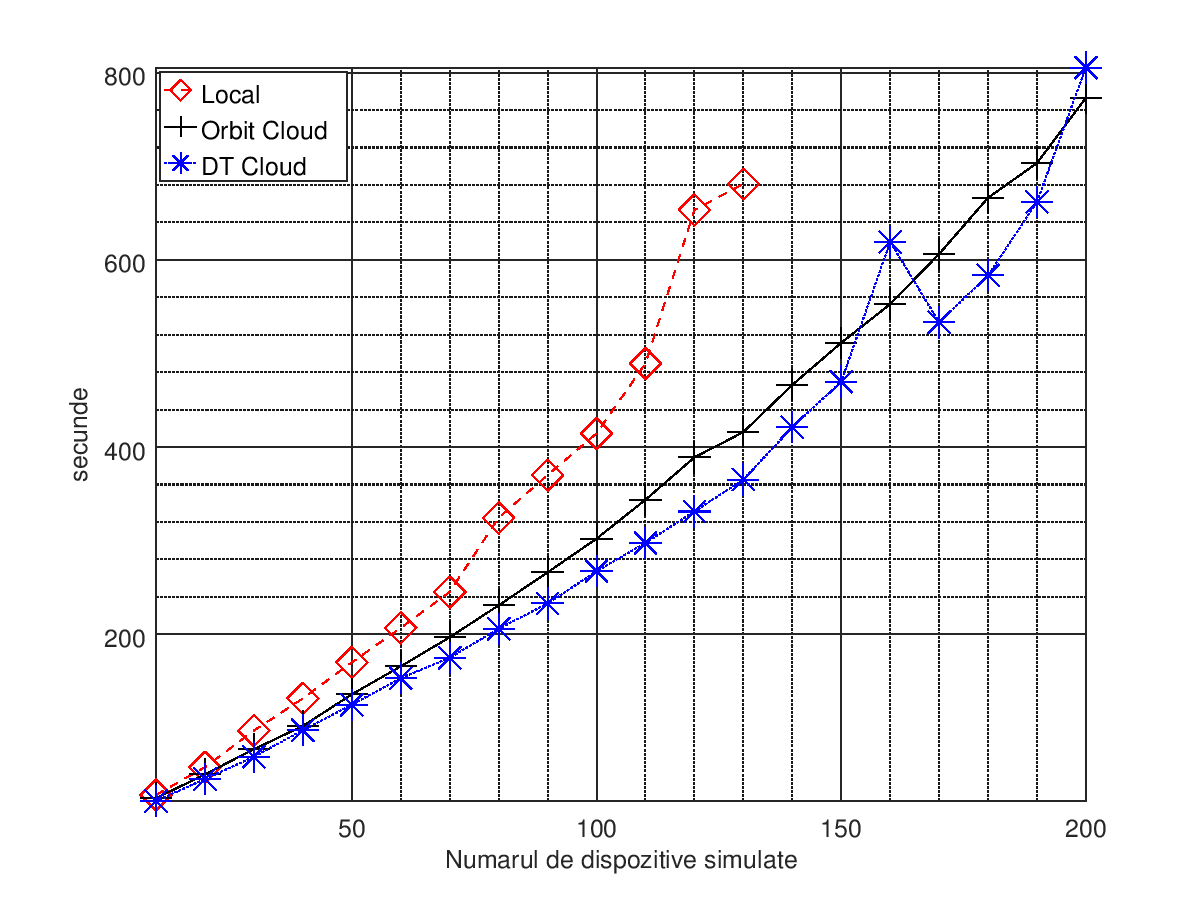
\includegraphics[width=0.85\textwidth]{boot_vs_ne_ring_v2}
	\caption{Timpul de iniţializare în funcție de numărul de dispozitive de rețea simulate, într-o rețea de tip \textbf{inel}, după optimizarea operaţiilor de pornire}
	\label{fig:boot_vs_ne_ring_v2}
\end{figure}

\begin{figure}[hp]
	\centering
	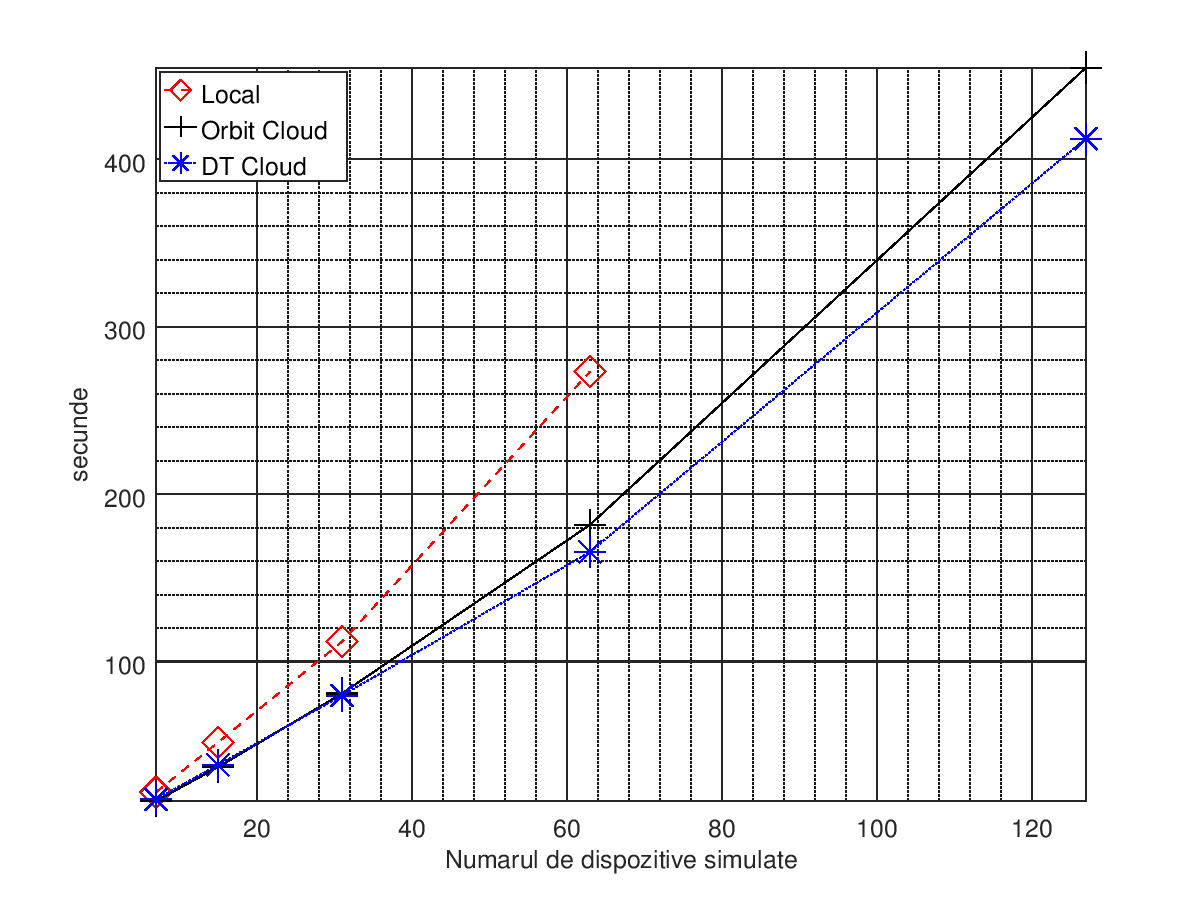
\includegraphics[width=0.85\textwidth]{boot_vs_ne_tree_v2}
	\caption{Timpul de iniţializare în funcție de numărul de dispozitive de rețea simulate, într-o rețea de tip \textbf{arbore}, după optimizarea operaţiilor de pornire}
	\label{fig:boot_vs_ne_tree_v2}
\end{figure}

\begin{figure}[hp]
	\centering
	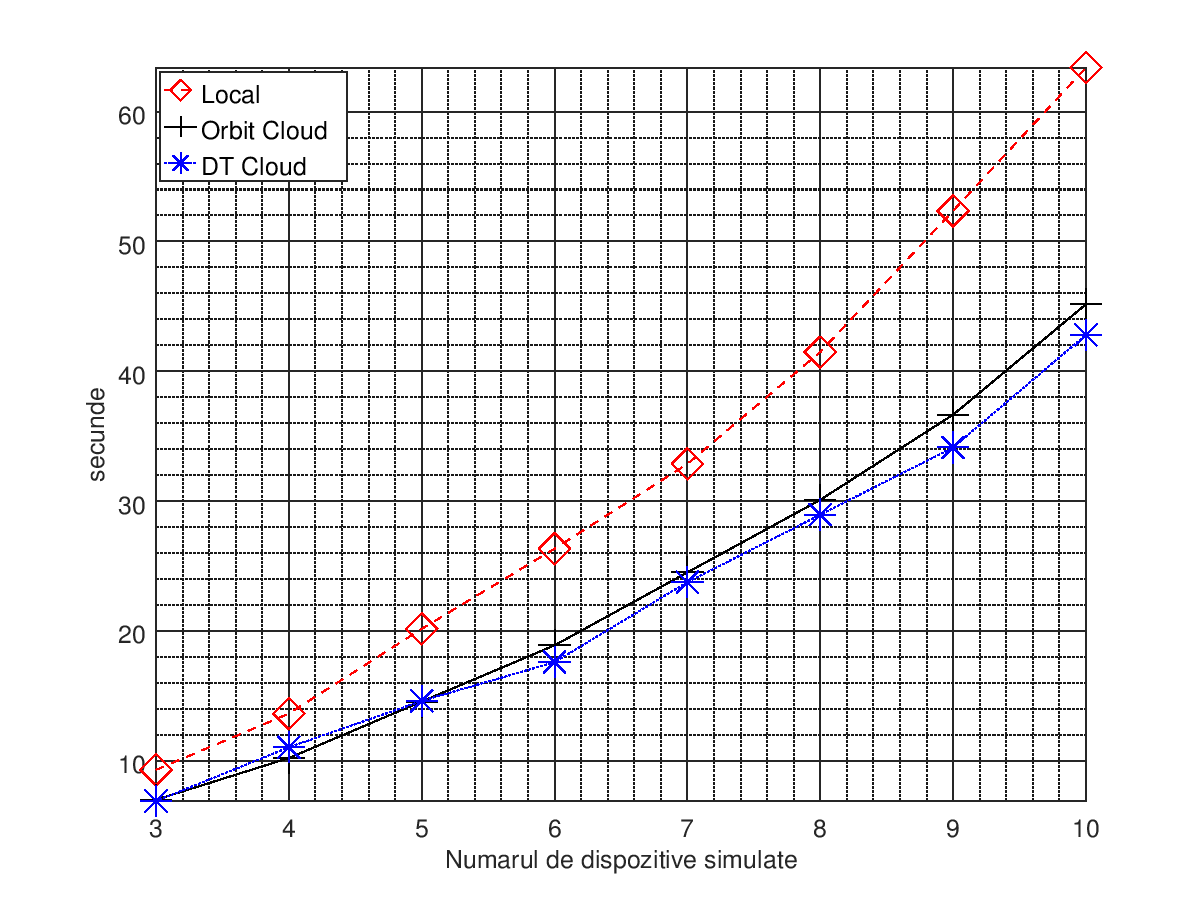
\includegraphics[width=0.85\textwidth]{boot_vs_ne_mesh_v2}
	\caption{Timpul de iniţializare în funcție de numărul de dispozitive de rețea simulate, într-o rețea de tip \textbf{plasă}, după optimizarea operaţiilor de pornire}
	\label{fig:boot_vs_ne_mesh_v2}
\end{figure}

\subsection{Spaţiul ocupat pe disc}

Următoarea caracteristică măsurată pentru \gls{wte} a fost spaţiul pe care topologiile simulate îl ocupă pe disc. Acesta este dat de utilitarul \textit{docker}, care are nevoie de el pentru reprezentarea sistemului de fişiere din interiorul fiecărui container \textit{docker}, dar și pentru salvarea informaţiilor despre interfeţele Linux reprezentate în fiecare container. Rezultatele măsurătorilor sunt ilustrate în Figurile~\ref{fig:storage_vs_ne_ring}, \ref{fig:storage_vs_ne_tree}, \ref{fig:storage_vs_ne_mesh} și \ref{fig:storage_vs_intf_mesh}.

\begin{figure}[hp]
	\centering
	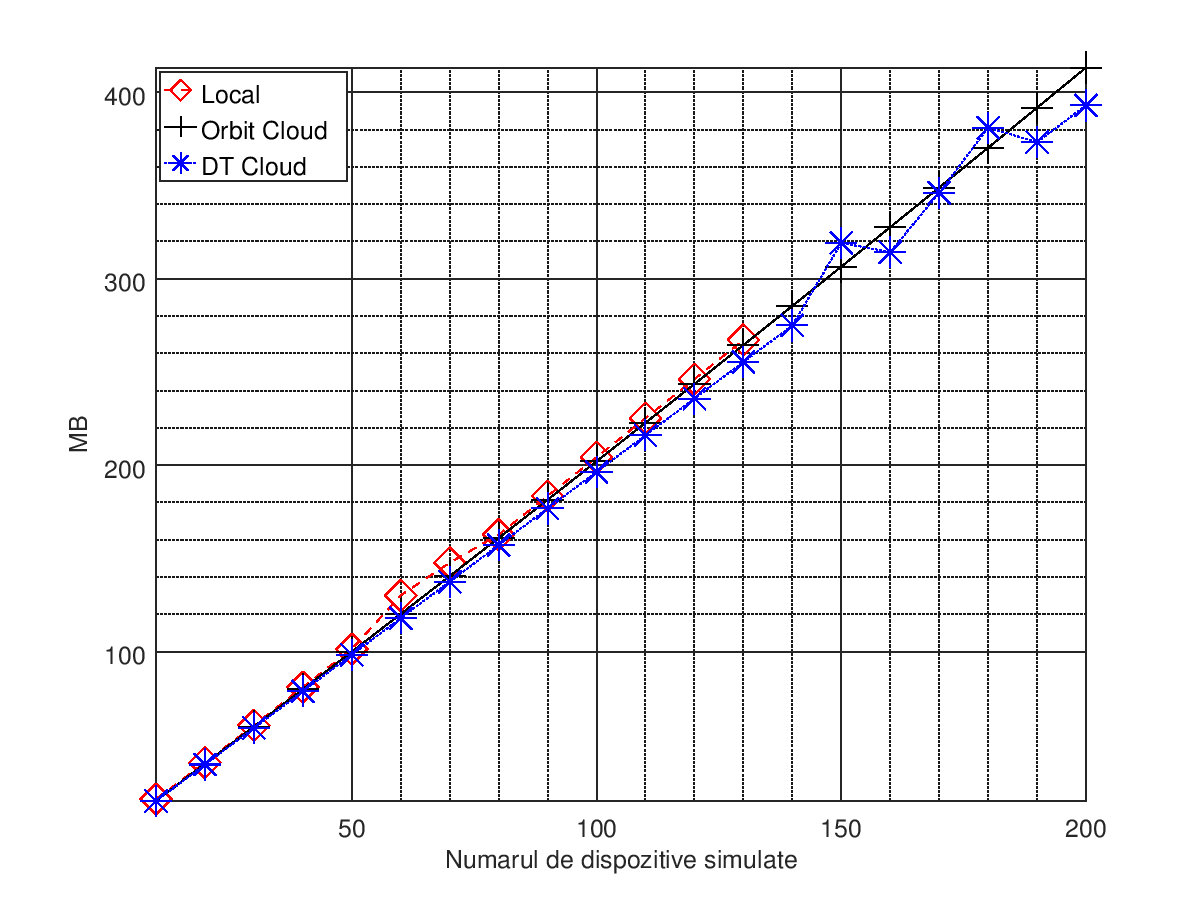
\includegraphics[width=0.85\textwidth]{storage_vs_ne_ring}
	\caption{Spaţiul de stocare utilizat în funcție de numărul de dispozitive de rețea simulate, într-o rețea de tip \textbf{inel}}
	\label{fig:storage_vs_ne_ring}
\end{figure}

\begin{figure}[hp]
	\centering
	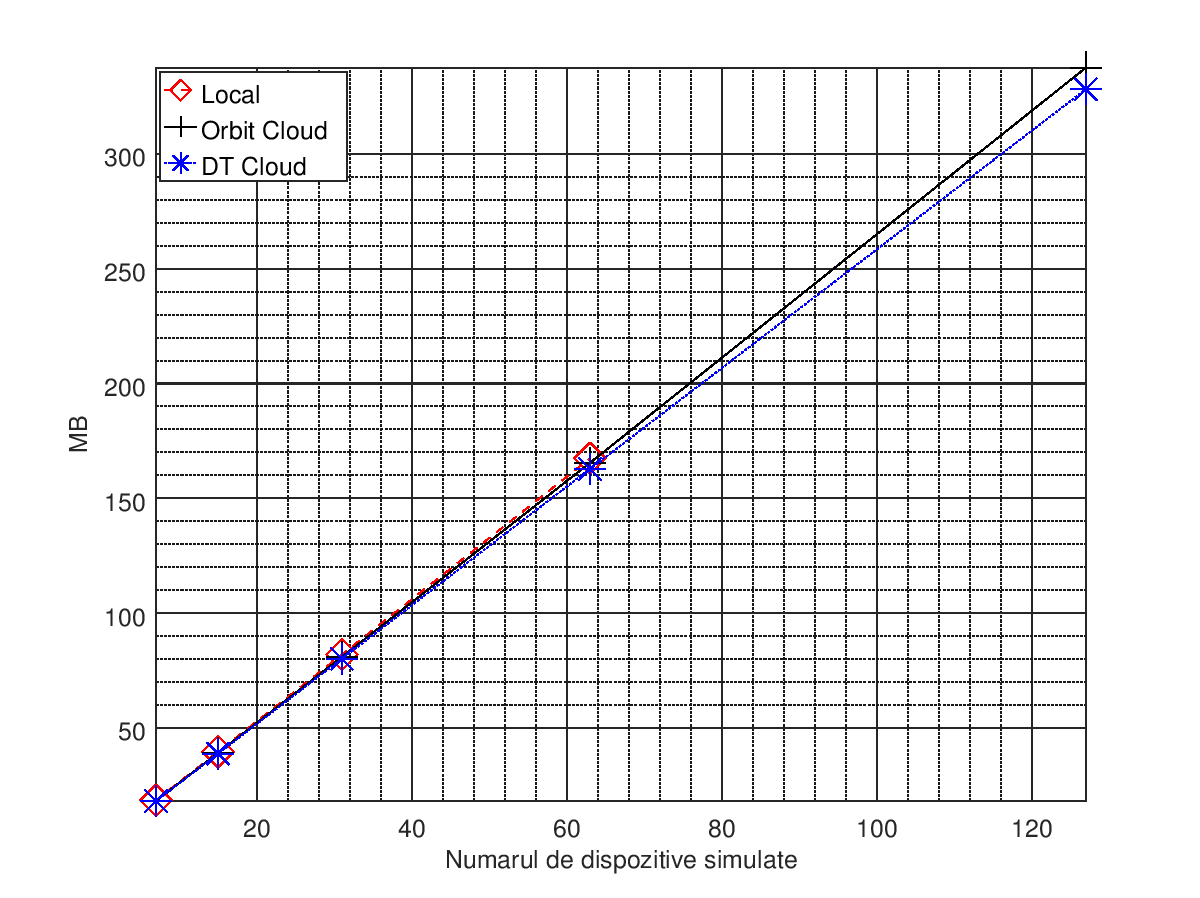
\includegraphics[width=0.85\textwidth]{storage_vs_ne_tree}
	\caption{Spaţiul de stocare utilizat în funcție de numărul de dispozitive simulate, într-o rețea de tip \textbf{arbore}}
	\label{fig:storage_vs_ne_tree}
\end{figure}

\begin{figure}[hp]
	\centering
	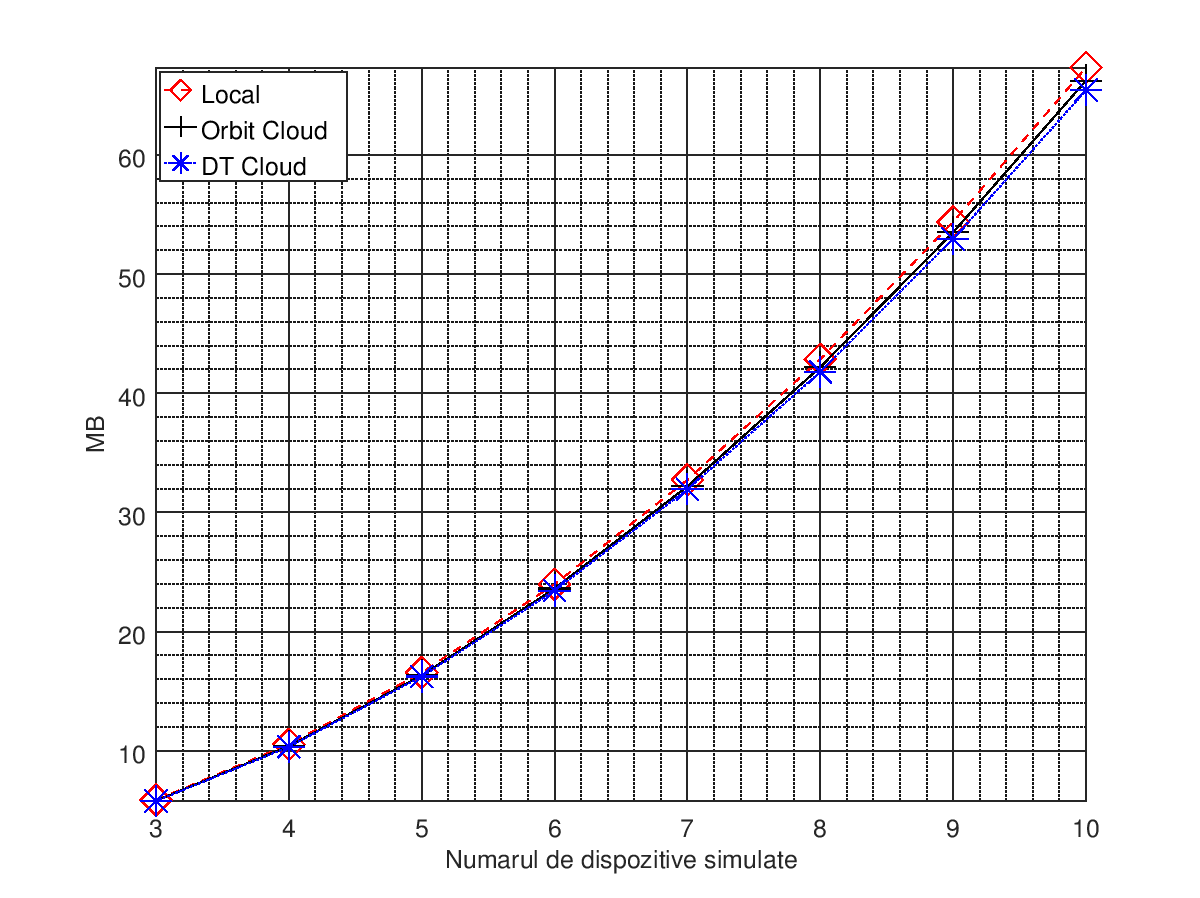
\includegraphics[width=0.85\textwidth]{storage_vs_ne_mesh}
	\caption{Spaţiul de stocare utilizat în funcție de numărul de dispozitive de rețea simulate, într-o rețea de tip \textbf{plasă}}
	\label{fig:storage_vs_ne_mesh}
\end{figure}

\begin{figure}[hp]
	\centering
	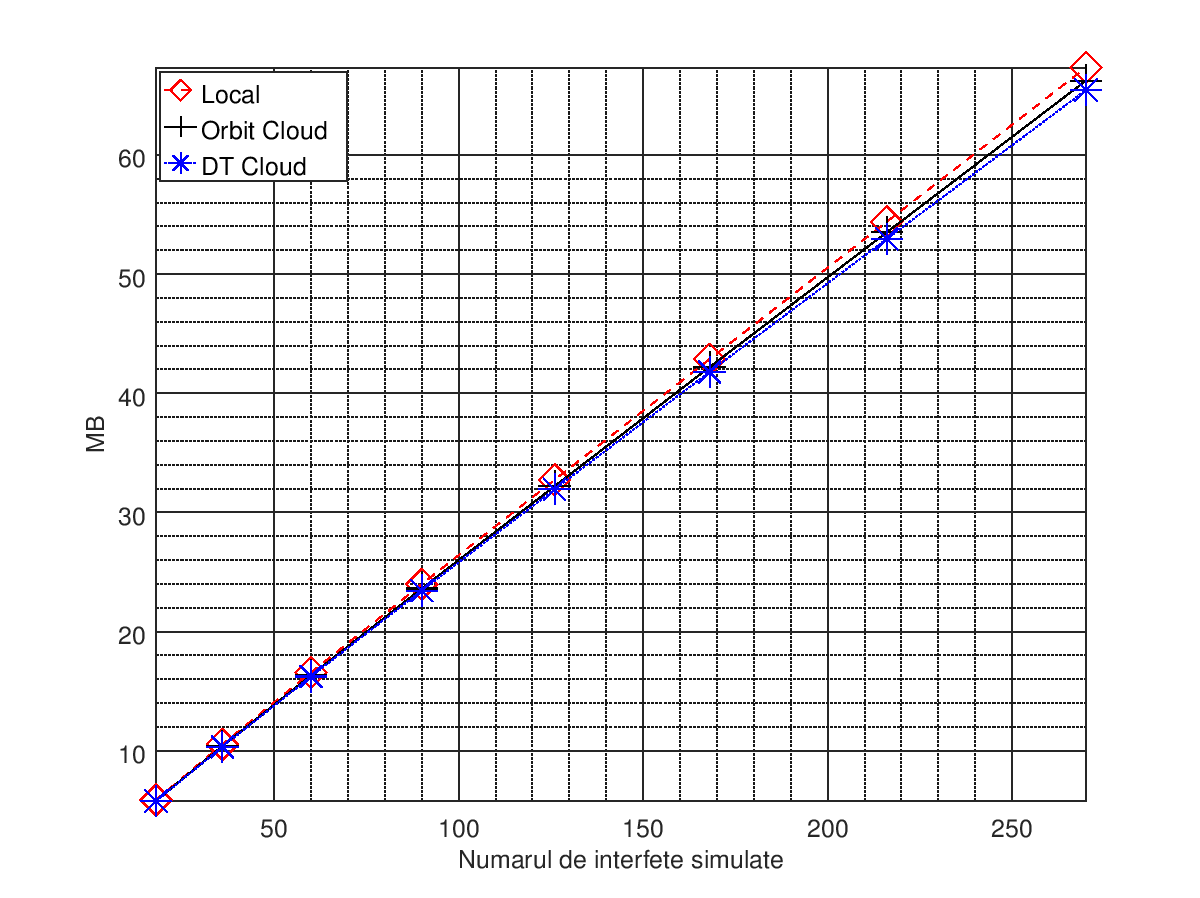
\includegraphics[width=0.85\textwidth]{storage_vs_intf_mesh}
	\caption{Spaţiul de stocare utilizat în funcție de numărul de interfețe simulate, într-o rețea de tip \textbf{plasă}}
	\label{fig:storage_vs_intf_mesh}
\end{figure}

Aceste figuri relevă faptul că spaţiul de stocare depinde liniar în principal de numărul de interfețe simulate, după cum se poate observa foarte clar în Figurile~\ref{fig:storage_vs_ne_mesh} și \ref{fig:storage_vs_intf_mesh}. În graficul ce reprezintă spaţiul de stocare în funcție de numărul de dispozitive simulate într-o topologie de tip plasă se poate observa o dependenţă pătratică, în timp ce în graficul ce prezintă spaţiul de stocare în funcție de numărul de interfețe simulate, în topologia de tip plasă, această dependenţă este liniară, de unde concluzia că această caracteristică măsurată depinde în principal de numărul interfeţelor simulate.

În cazul rețelelor de tip inel, la un număr de aproximativ 120 de dispozitive simulate, însemnând 960 de interfețe simulate, spaţiul de stocare ocupat de \gls{wte} ajunge în jurul valorii de 240 MB, pentru rețelele de tip arbore cu un număr de 120 de dispozitive simulate, adică aproximativ 1270 de interfețe simulate, sunt utilizaţi aproximativ 330 MB. Pentru rețelele de tip plasă, la un număr de 10 dispozitive simulate, având 270 de interfețe simulate, spaţiul pe disc utilizat ajunge la 65 MB. Practic, aceste valori duc la o medie aproximativă de 0,25 MB per interfață simulată.

\subsection{Puterea de procesare folosită}

Caracteristicile măsurate anterior nu sunt foarte importante după ce simulatorul a fost pornit: timpul de iniţializare nu mai e relevant, iar spaţiul de stocare nu are valori atât de mari (în funcție de topologie ajunge la zeci sau sute de MB) încât sa fie o problemă pe majoritatea maşinilor de calcul din zilele noastre. Însă, puterea de procesare și procentul memoriei cu acces aleator sunt caracteristici importante, deoarece limitează practic topologiile ce pot fi simulate pe un sistem.

Puterea de procesare măsurată este reprezentată ca procentul de folosire a procesorului, raportat la puterea totală de procesare a sistemului. De exemplu, dacă avem un procesor cu patru nuclee, iar simulatorul ar avea o putere de procesare folosită de 25\%, ar însemna că un nucleu este folosit în exclusivitate de către \gls{wte}.

Rezultatele măsurătorilor puterii de procesare folosită sunt ilustrate în Figurile~\ref{fig:cpu_vs_intf_ring}, \ref{fig:cpu_vs_intf_tree} și \ref{fig:cpu_vs_intf_mesh}.

\begin{figure}[hp]
	\centering
	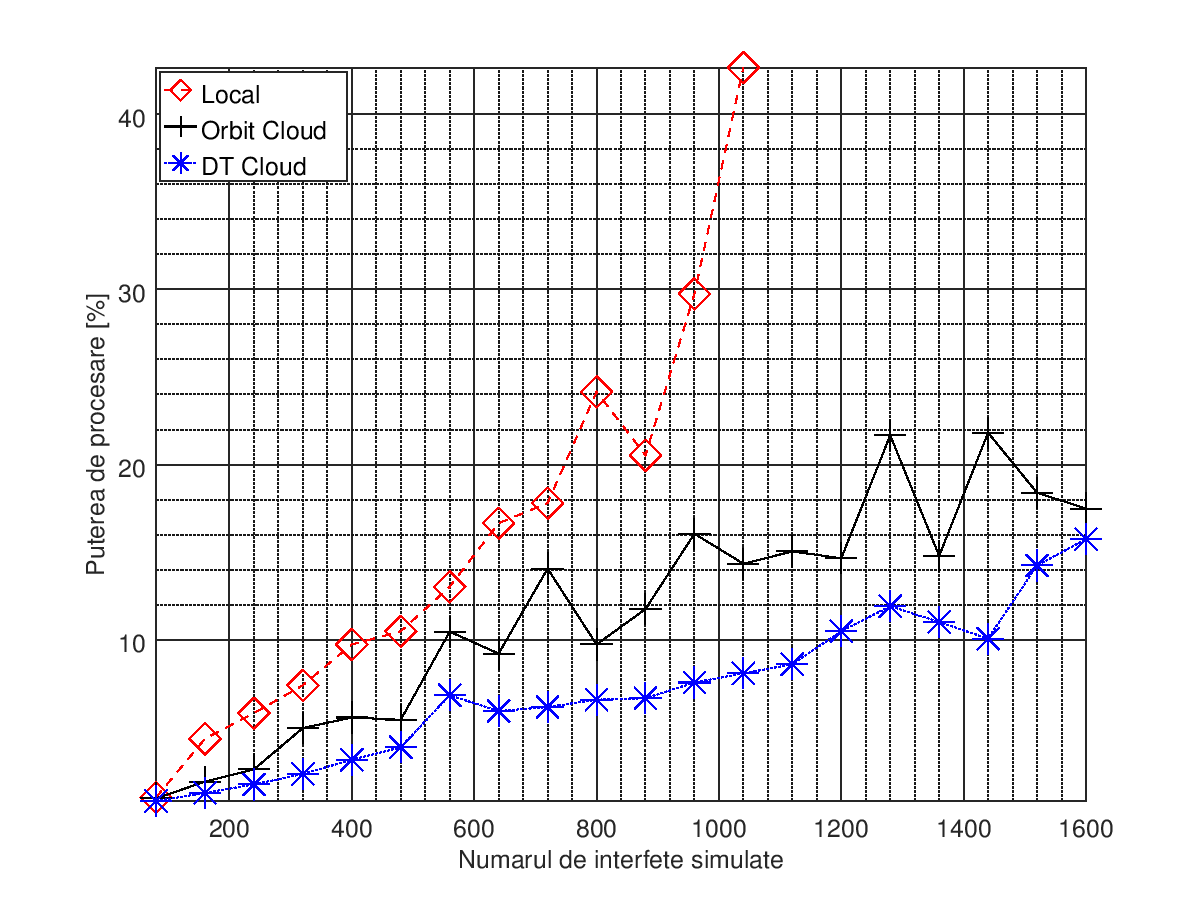
\includegraphics[width=0.85\textwidth]{cpu_vs_intf_ring}
	\caption{Puterea de procesare folosită în funcție de numărul de interfețe simulate, într-o rețea de tip \textbf{inel}}
	\label{fig:cpu_vs_intf_ring}
\end{figure}

\begin{figure}[hp]
	\centering
	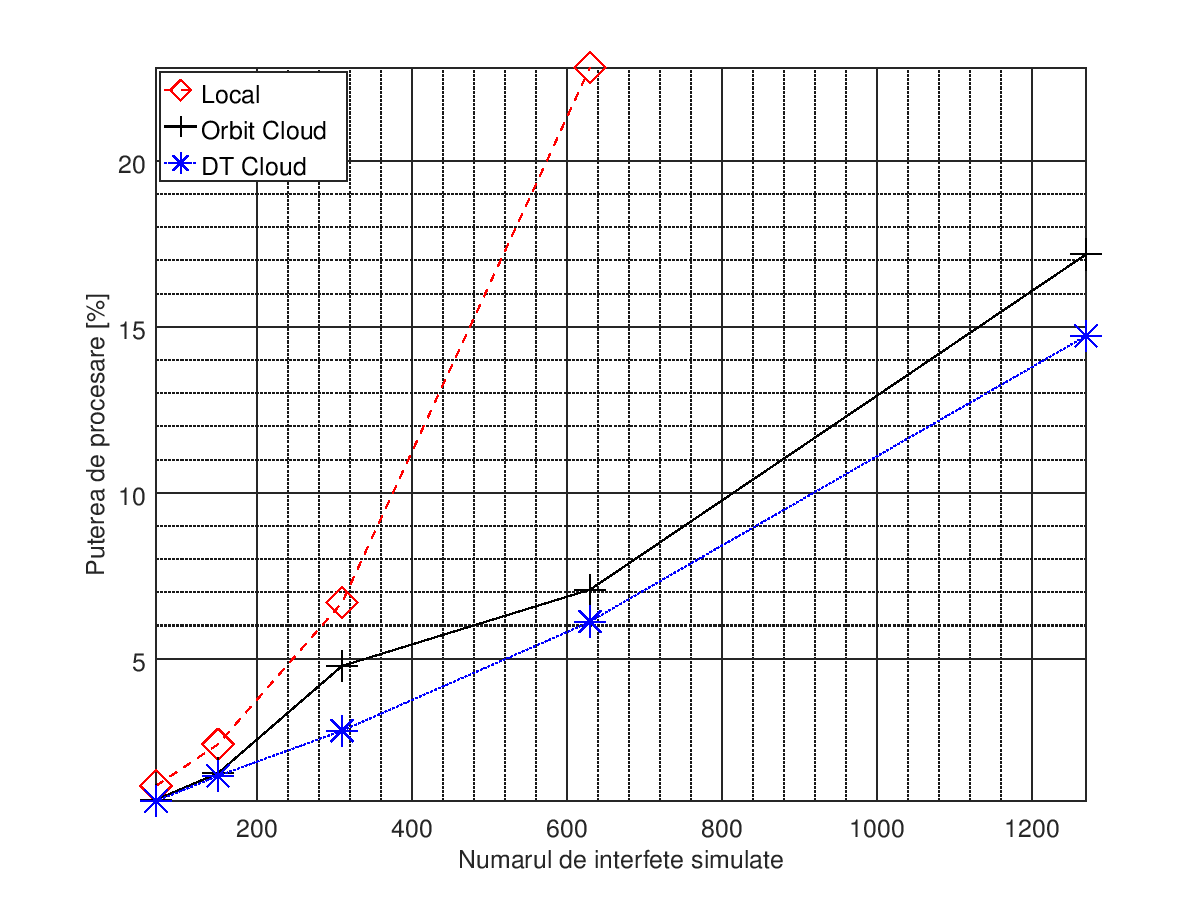
\includegraphics[width=0.85\textwidth]{cpu_vs_intf_tree}
	\caption{Puterea de procesare folosită în funcție de numărul de interfețe simulate, într-o rețea de tip \textbf{arbore}}
	\label{fig:cpu_vs_intf_tree}
\end{figure}

\begin{figure}[hp]
	\centering
	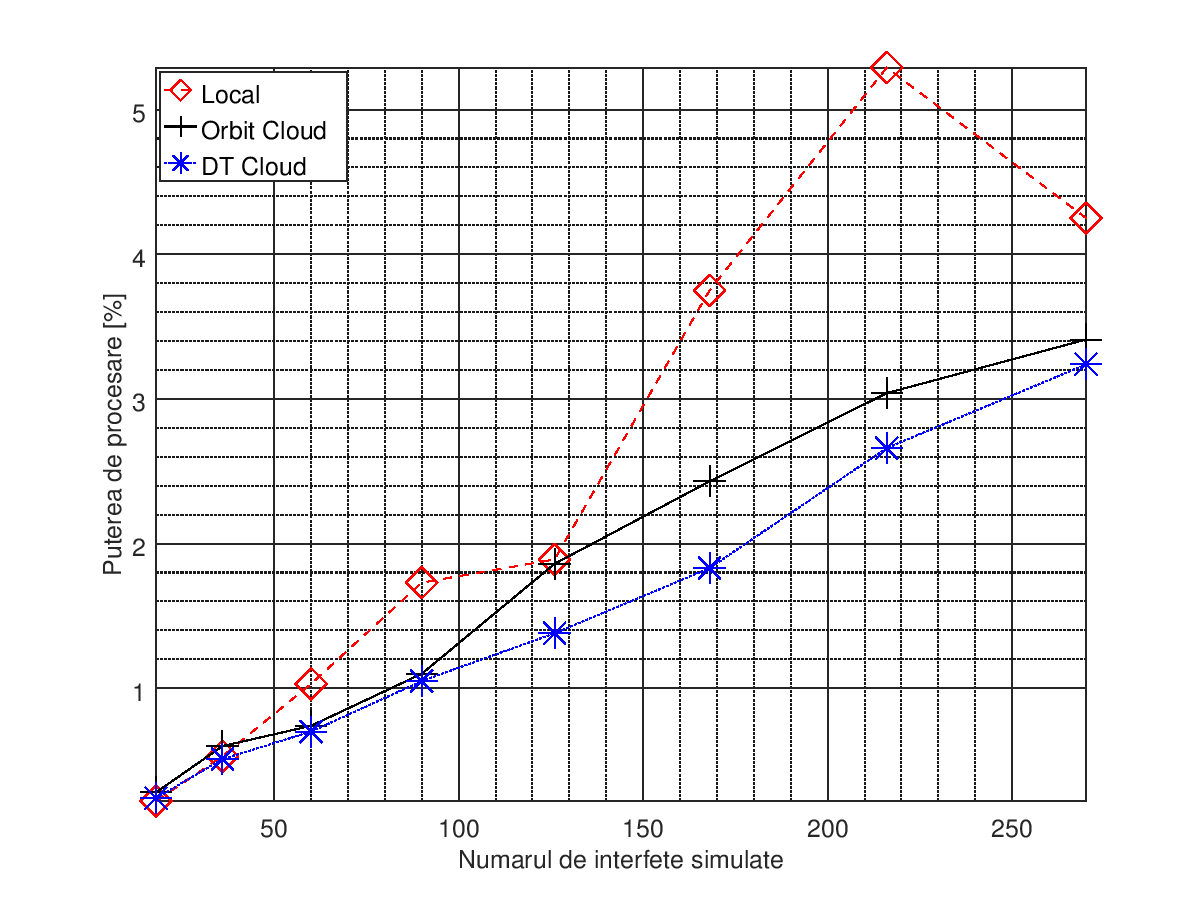
\includegraphics[width=0.85\textwidth]{cpu_vs_intf_mesh}
	\caption{Puterea de procesare folosită în funcție de numărul de interfețe simulate, într-o rețea de tip \textbf{plasă}}
	\label{fig:cpu_vs_intf_mesh}
\end{figure}

Se poate observa, cu ajutorul acestor măsurători, că puterea de procesare folosită de către \gls{wte}, chiar prin măsurarea mai multor eşantioane și calcularea unei valori medii, nu are o variaţie perfect liniară cu una dintre variabilele prezente în diferitele topologii (numărul de dispozitive, numărul de interfețe sau numărul de legături de date). Măsurătorile din cele două medii de tip \textit{cloud} (Orbit si DT) au tendinţe asemănătoare, chiar dacă variaţia puterii de procesare nu este perfect liniară cu numărul de interfețe simulate. Măsurătorile locale, însă, de la un punct, nu mai respectă această tendinţă liniară. Cel mai probabil, acest lucru este influenţat de nivelul în plus de virtualizare, dat de maşina Linux pe care este instalat mediul de simulare \gls{wte}.

Pentru un număr de 250 de interfețe simulate, în cazul topologiei de tip plasă, puterea de procesare utilizată de \gls{wte} ajunge la aproximativ 3\%, pentru un număr de 1200 de interfețe simulate, în cazul topologiei de tip inel, puterea de procesare folosită se situează în jurul valorii de 12\%, în timp ce pentru același număr de interfețe în cazul topologiei de tip arbore simulatorul utilizează aproximativ 14\% din puterea de procesare a sistemului.

Un alt scenariu a fost considerat pentru a măsura influenţa injectării de trafic în rețeaua simulată asupra puterii de procesare de care \gls{wte} are nevoie. Acesta a constat în simularea unei topologii de tip plasă cu redundanţă maximă cu 10 dispozitive, așa cum se poate observa în Figura~\ref{fig:mesh_topo_traffic}. Pentru ca figura să nu fie încărcată în mod excesiv, au fost ilustrate doar legăturile de date prin care trece traficul dintre dispozitivele de rețea.

\begin{figure}[hp]
	\centering
	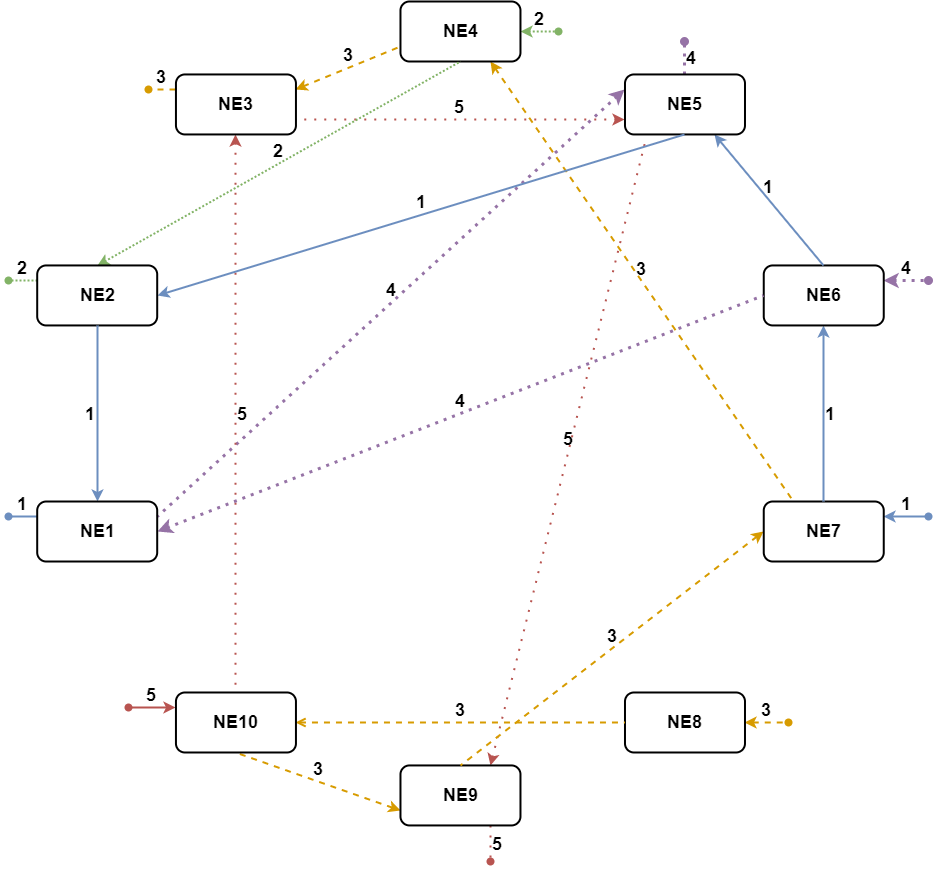
\includegraphics[width=1\textwidth]{mesh_topo_traffic}
	\caption{Topologie de tip plasă în care sunt reprezentate fluxurile de trafic simulate}
	\label{fig:mesh_topo_traffic}
\end{figure}

Primul pas a fost măsurarea puterii de procesare utilizată de topologia simulată în condiţiile în care nu era injectat niciun flux de trafic. Apoi, a fost măsurată puterea de procesare în cazul în care se folosea un flux de trafic, apoi două, până la cinci fluxuri, conform figurii anterioare.

Figura~\ref{fig:cpu_mesh_traffic} prezintă valorile cu care puterea de procesare folosită de \gls{wte} creşte față de cazul fără trafic, în funcție de numărul de fluxuri de trafic ce se transmit în paralel prin rețeaua simulată.

\begin{figure}[hp]
	\centering
	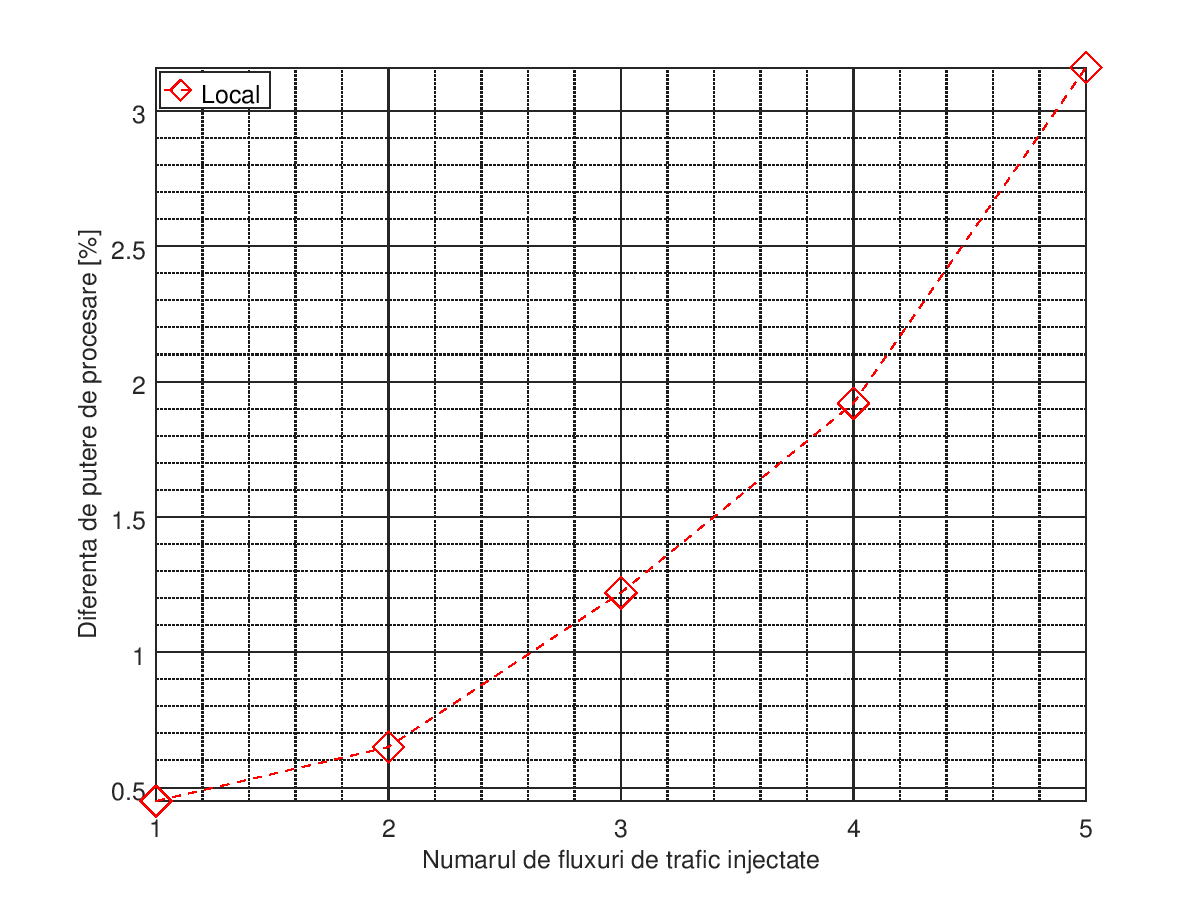
\includegraphics[width=0.8\textwidth]{cpu_mesh_traffic}
	\caption{Puterea de procesare de care injectarea de trafic are nevoie, într-o rețea de tip plasă cu redundanţă maximă, în funcție de numărul de fluxuri de trafic injectate în rețea}
	\label{fig:cpu_mesh_traffic}
\end{figure}

Putem observa că puterea de procesare folosită pentru transmiterea de trafic în rețeaua simulată creşte exponenţial cu numărul de fluxuri injectate, ajungând la 3\% pentru 5 astfel de conexiuni. Aceasta este utilizată de serverele și clienţii utilitarului \textit{iperf} asociaţi cu aceste operații de transfer de date.

\subsection{Memoria cu acces aleator}

Ultima caracteristică măsurată pentru \gls{wte} este reprezentată de procentul de memorie cu acces aleator folosit de către simulator, raportat la totalul memoriei cu acces aleator disponibilă în sistem. Aceasta este practic cea mai importantă caracteristică folosită de \gls{wte}, care va limita de fapt numărul de dispozitive de rețea sau interfețe ce pot fi simulate. Dacă în cazul procentului de putere de procesare, în cazul în care simulatorul are nevoie de un procent mare, acestuia îi va reveni, la un moment dat și simulatorul va fi executat în continuare de către sistemul de operare, chiar dacă execuţia întregului sistem va deveni greoaie, în cazul procentului de memorie cu acces aleator, dacă \gls{wte} va mai încerca să aloce memorie și sistemul nu îi mai poate îndeplini cererea, execuţia simulatorului va fi terminată de către sistemul de operare.

Rezultatele măsurătorilor procentului de memorie cu acces aleator folosită de simulatorul \gls{wte} sunt prezentate în Figurile~\ref{fig:mem_vs_intf_ring}, \ref{fig:mem_vs_intf_tree} și \ref{fig:mem_vs_intf_mesh}.

\begin{figure}[hp]
	\centering
	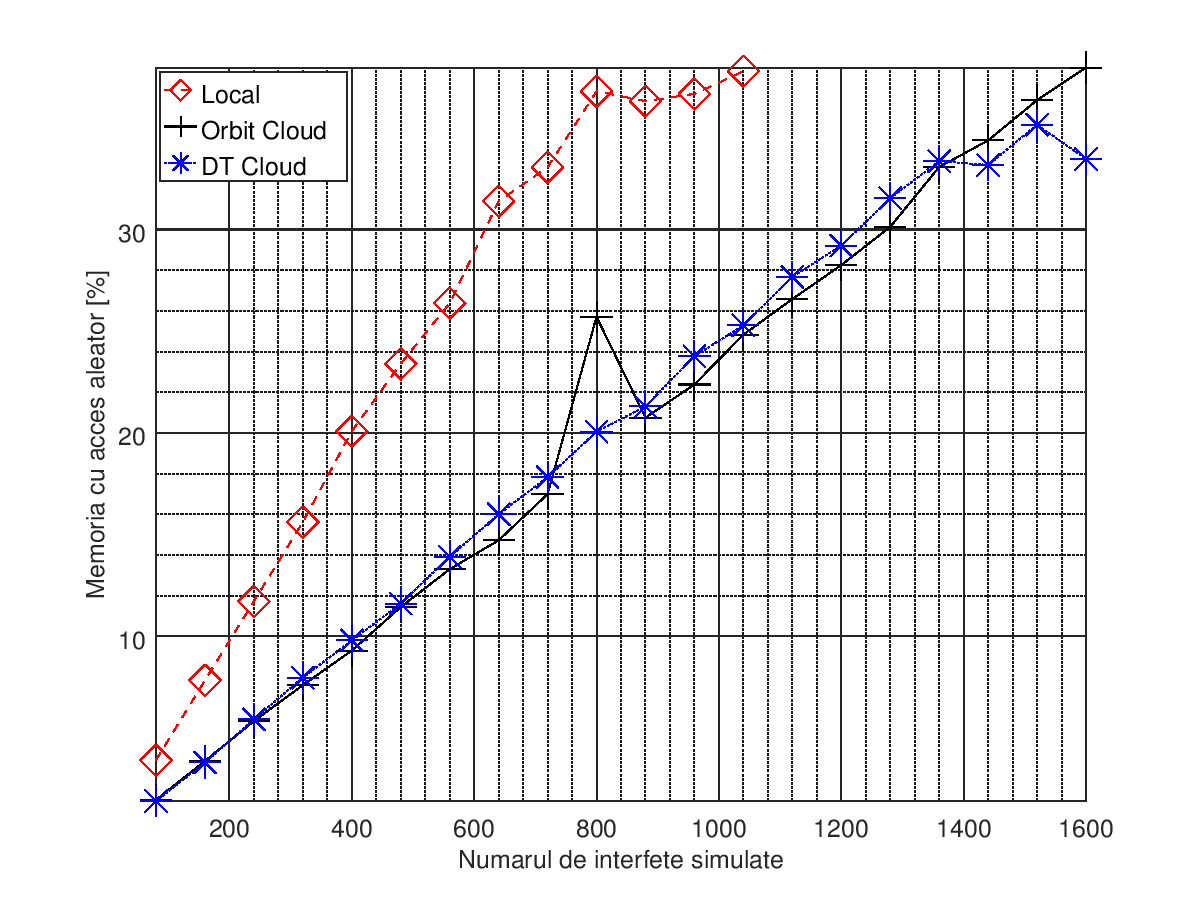
\includegraphics[width=0.85\textwidth]{mem_vs_intf_ring}
	\caption{Memoria cu acces aleator folosită în funcție de numărul de interfețe simulate, într-o rețea de tip \textbf{inel}}
	\label{fig:mem_vs_intf_ring}
\end{figure}

\begin{figure}[hp]
	\centering
	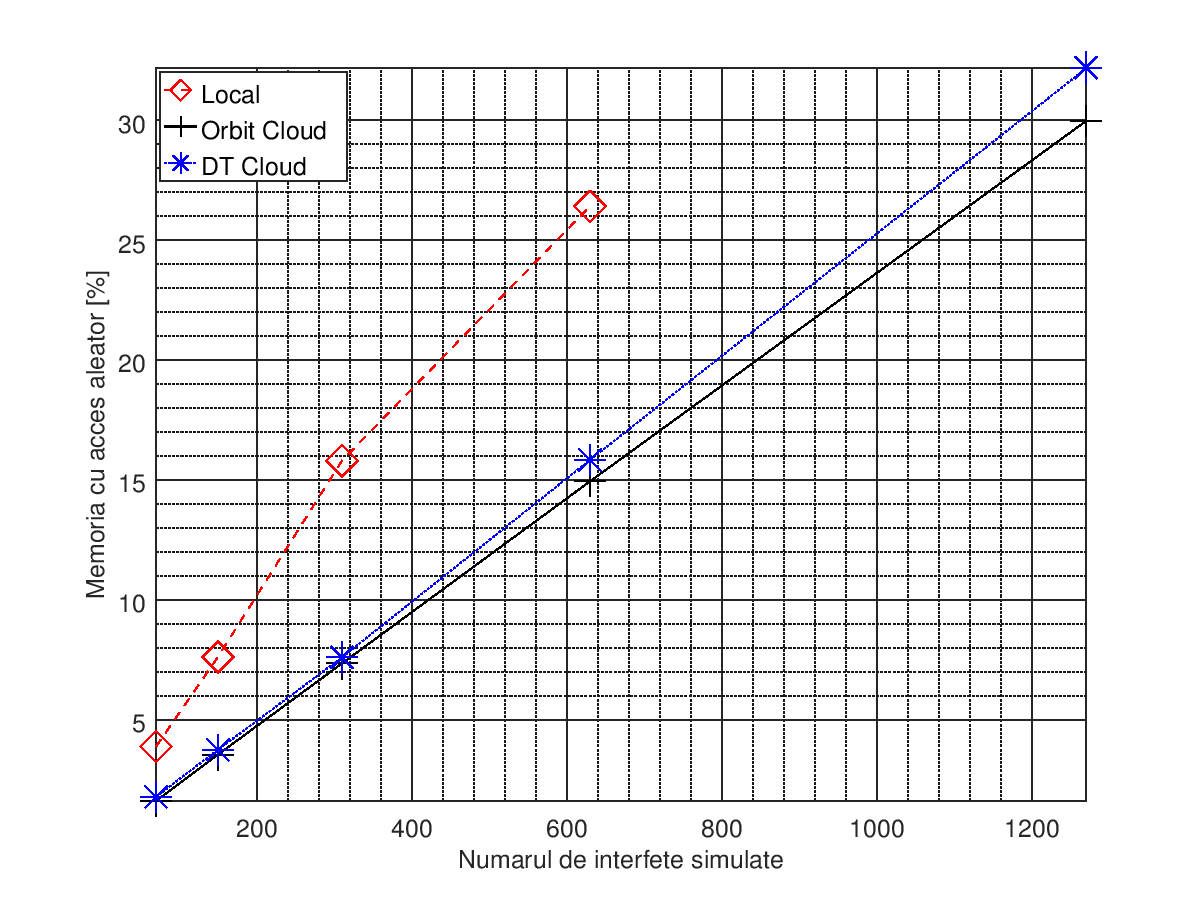
\includegraphics[width=0.85\textwidth]{mem_vs_intf_tree}
	\caption{Memoria cu acces aleator folosită în funcție de numărul de interfețe simulate, într-o rețea de tip \textbf{arbore}}
	\label{fig:mem_vs_intf_tree}
\end{figure}

\begin{figure}[hp]
	\centering
	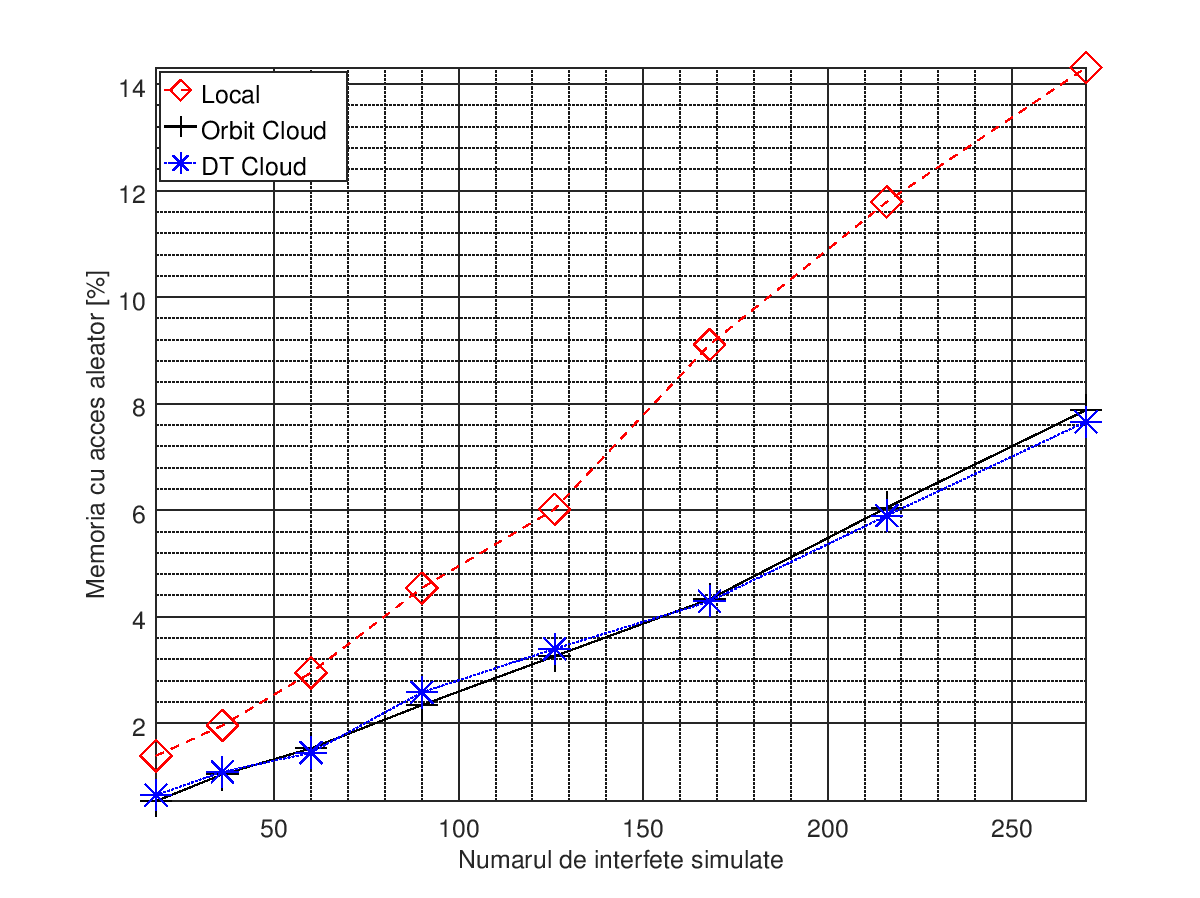
\includegraphics[width=0.85\textwidth]{mem_vs_intf_mesh}
	\caption{Memoria cu acces aleator folosită în funcție de numărul de interfețe simulate, într-o rețea de tip \textbf{plasă}}
	\label{fig:mem_vs_intf_mesh}
\end{figure}

Se observă o dependenţă liniară între numărul de interfețe simulate și procentul de memorie cu acces aleator folosită de \gls{wte}. În exemplele următoare considerăm mediile de simulare de tip \textit{cloud}, care au 8 GB de memorie cu acces aleator. Pentru topologia de tip plasă, la un număr de 200 de interfețe simulate, procentul de memorie cu acces aleator utilizat de simulator ajunge la aproximativ 5\%. Pentru topologia arbore, la 1000 de interfețe simulate, valoarea procentului de memorie cu acces aleator ajunge la aproximativ 24\%, iar în cazul topologiei de tip inel, pentru același număr de interfețe, această valoare ajunge tot în jurul pragului de 24\%. Putem concluziona astfel că, indiferent de topologia simulată, \gls{wte} are nevoie de aproximativ 0,025\% memorie cu acces aleator pentru fiecare interfață pe care o va simula, adică 2 MB, având în vedere că am considerat cazul în care sistemul dispune de un total de 8 GB.

\subsection{Concluziile evaluării}

Rezultatele evaluării ilustrează câteva concluzii interesante despre \gls{wte}. Variabila care influenţează cel mai mult comportamentul simulatorului nu este numărul de dispozitive de rețea simulate, așa cum poate era de așteptat, ci numărul de interfețe pe care topologia le conţine. Cu cât acest număr este mai mare, cu atât timpul de iniţializare a simulatorului, memoria cu acces aleator utilizată și spaţiul pe disc necesar sunt mai mari.

Timpul de iniţializare a simulatorului este destul de mare în cazul topologiilor mari, ajungând la sute de secunde pentru rețele care conţin mii de interfețe. Acest timp nu este critic pentru funcționarea \gls{wte}, deoarece, odată pornit, simulatorul nu mai are nevoie să fie redeschis decât în cazul în care se doreşte schimbarea topologiei simulate. Influenţează, însă, experienţa de folosire pe care o are utilizatorul. După ce s-a optimizat iniţializarea \gls{wte} prin gruparea creării interfeţelor Linux asociate obiectelor \gls{ltp}, timpul de iniţializare a fost îmbunătăţit semnificativ, dar este influenţat în continuare în principal de durata creării și pornirii containerelor \textit{docker} asociate dispozitivelor de rețea simulate. Acest timp nu poate fi îmbunătăţit, deoarece utilitarul \textit{docker} nu permite paralelizarea acestor operații.

Spaţiul de stocare pe disc nu pare să reprezinte o problemă în folosirea \gls{wte}, chiar și în cazul simulării unor topologii de rețea foarte mari. Acesta depinde de numărul de interfețe, simulatorul având nevoie de aproximativ 0,25 MB pentru fiecare interfață simulată. Astfel, pentru o rețea ce conţine 4000 de interfețe, \gls{wte} va folosi aproximativ 1 GB de memorie pe disc, ceea ce nu reprezintă o problemă pentru majoritatea sistemelor din zilele noastre.

Memoria cu acces aleator necesară pentru execuţia \gls{wte} prezintă o dependenţă liniară de numărul de interfețe simulate. Conform rezultatelor prezentate anterior, indiferent de tipul de topologie care este simulată, \gls{wte} are nevoie de aproximativ 2 MB de memorie cu acces aleator pentru fiecare interfață care trebuie reprezentată.

Puterea de procesare este caracteristica simulatorului care variază cel mai mult și cel mai puţin predictibil. Observăm o creștere a acesteia cu numărul de dispozitive de rețea simulate, cu numărul de interfețe dar și cu numărul de fluxuri de trafic ce se injectează în rețea. Această caracteristică nu este predictibilă, deoarece utilitarul \textit{docker} este responsabil de alocarea de putere de procesare fiecărui container, în funcție de nevoile acestuia. În timpul execuţiei, aceste nevoi pot varia și în funcție de aplicațiile din echipamentul de control \gls{sdn} care administrează rețeaua.

Dimensiunea topologiilor ce pot fi simulate este dată astfel, în principal, de cantitatea de memorie cu acces aleator care este disponibilă pe sistemul unde a fost instalat mediul de simulare. În cazul unui sistem cu 4 GB de astfel de memorie, pot fi simulate până la 1000 de interfețe. Chiar dacă, conform măsurătorilor efectuate anterior, aceste 1000 de interfețe ar ocupa doar 2 GB din memoria cu acces aleator a sistemului, nu se poate folosi mai multă memorie, deoarece aceasta este folosită și de sistemul de operare și de alte eventuale aplicații care sunt executate în sistem. Pentru sisteme mai capabile, cu 8 GB de memorie cu acces aleator, numărul interfeţelor simulate poate depăşi 2500. Acestea se referă la interfeţele Linux asociate obiectelor \gls{ltp} din modelele informaționale propuse de \gls{onf}. Dacă ne referim doar la interfeţele de rețea prin care se fac legături în topologiile simulate, având în vedere că o astfel de interfață (de tip \gls{mwps}) are asociate încă două obiecte (de tip \gls{mws} și \gls{etc}), atunci putem afirma că se pot simula aproximativ 800 de astfel de interfețe.

Cu ajutorul acestei evaluări, a fost demonstrat că \gls{wte} poate reprezenta o soluție viabilă pentru dezvoltatorii de aplicații \gls{sdn}. Acesta permite simularea unor topologii diverse, care, în funcție de capabilitățile sistemului pe care este instalat, pot fi destul de mari, ajungând să conţină mii de interfețe de rețea. Astfel, dezvoltatorii pot executa și teste de extensibilitate pentru aplicațiile pe care le implementează. Chiar dacă rețelele reale, de producție, pot conţine mii de elemente și zeci de mii de interfețe, \gls{wte} este un prim pas pentru simularea unor astfel de rețele de transport de date fără fir, în contextul \gls{sdn}. În viitor, acest simulator se poate optimiza, astfel încât să permită reprezentarea unor astfel de rețele, la scara la care există în producție, sau se poate căuta o soluție în care \gls{wte} să fie executat în mod distribuit, pe mai multe sisteme.
\section{Alte abordări}

Simulatorul care constituie baza acestei lucrări, \gls{wte}, oferă o interfață \gls{netconf} care implementează modelele informaționale dezvoltate de \gls{onf}, TR-512 și TR-532, în contextul \gls{sdn} în rețelele de transport de date fără fir. Acestea sunt apărute destul de recent, astfel încât nu există încă unelte care să simuleze asemenea topologii și să expună modelele informaționale echipamentelor de control \gls{sdn}.

Majoritatea simulatoarelor folosite pentru crearea de topologii de rețele definite prin software se bazează pe protocolul OpenFlow și sunt reprezentate de: \textit{mininet}, \textit{EstiNet} și \textit{ns-3}~\cite{lantz2010network,wang2013estinet,wang2014comparison,henderson2008network}. În continuare se va compara simulatorul \gls{wte} cu \textit{mininet}, deoarece acesta este cel mai folosit simulator în contextul \gls{sdn}~\cite{brandonheller2013}.

Din punct de vedere arhitectural, \gls{wte} este foarte asemănător cu \textit{mininet}. Ambele se bazează pe un nucleu Python care se ocupă de toate aspectele simulării: crearea de mașini gazdă, de comutatoare sau de legături între acestea, prin perechi Ethernet virtuale. Dacă în cazul \textit{mininet} se simulează mașini gazdă, sub forma unor procese, care apoi se leagă la comutatoarele din rețea, în cazul \gls{wte} se pune accent pe simularea de dispozitive de rețea și pe funcţionalitatea oferită de acestea echipamentului de control \gls{sdn}, prin intermediul protocolului \gls{netconf}.

Atât \textit{mininet}, cât și \gls{wte} folosesc, după iniţializarea topologiei ce se vrea a fi simulată, o interfață prin linie de comandă care aşteaptă comenzi de la utilizator. Aceasta are cunoştinţe cu privire la dispozitivele de rețea și legăturile dintre acestea și poate trimite comenzi echipamentelor sau poate informa utilizatorul cu privire la detalii despre starea acestora.

Chiar dacă oferă funcționalități diferite, \textit{mininet} oferind OpenFlow, iar \gls{wte} bazându-se pe \gls{netconf}, ambele tipuri de simulatoare folosesc conceptul de virtualizare bazată pe containere Linux~\cite{handigol2012reproducible}. În cazul \textit{mininet}, acestea sunt folosite în mod nativ, prin utilizarea lor directă în Linux. \gls{wte} folosește utilitarul \textit{docker} pentru a crea containere ce reprezintă dispozitive de rețea.

Abordările în cadrul celor două simulatoare, din punctul de vedere al alegerii topologiei care trebuie simulată, sunt diferite. \textit{Mininet} oferă posibilitatea de a porni simulatorul din linia de comandă, specificând prin anumiţi parametri tipul topologiei și dimensiunea acesteia. O altă posibilitate este crearea acesteia prin descrierea lor direct în codul Python, prin interfeţele de programare puse la dispoziţie. Simulatorul \gls{wte} prezintă altă abordare: descrierea topologiei într-un fişier de configurare, după un format prestabilit.

Din punct de vedere funcţional, cele două simulatoare folosesc aceeaşi metodă pentru reprezentarea legăturilor de rețea, perechi Ethernet virtuale, indiferent de punctele între care se doreşte legătura de date: între o mașină gazdă și un comutator, sau între două comutatoare, în cazul \textit{mininet}, sau între două dispozitive de rețea, în cazul \gls{wte}.

În cazul \gls{wte}, fiecare dispozitiv de rețea este reprezentat ca un container \textit{docker}, în interiorul căruia este executat serverul \gls{netconf}, folosit pentru a expune modelele informaționale dezvoltate de \gls{onf}. În cazul \textit{mininet}, pentru reprezentarea comutatoarelor OpenFlow se folosește implicit soluţia software \gls{ovs}, care este executată nativ (fără să fie nevoie de virtualizare) în mediul în care este instalat simulatorul, sau utilizatorul poate alege să folosească alt comutator software capabil să ofere protocolul OpenFlow. Din acest motiv, resursele consumate de către \gls{wte} sunt mai mari decât cele utilizate de \textit{mininet}. În schimb, din punctul de vedere al timpului de inițializare, \gls{wte} este mai eficient decât \textit{mininet}, după cum se poate observa comparând rezultatele măsurate cu rezultatele din~\cite{lantz2010network}.

Din punctul de vedere al traficului care se poate transmite în rețelele simulate, în ambele cazuri se poate injecta trafic cu ajutorul utilitarului \textit{iperf3}.
\section{Demonstrarea cazurilor de utilizare cu ajutorul WTE}

Standardizare: ONF, etc..
\chapter{Concluzii\label{ch:concluzii}}

Scopul acestei lucrări a fost dezvoltarea și implementarea unui mediu de simulare care să permită crearea de rețele de transport de date fără fir, care să poată fi folosite în contextul \gls{sdn} prin oferirea unei interfețe specifice \gls{netconf} ce expune modelele informaționale dezvoltate de \gls{onf} în acest sens. Simulatorul este destinat dezvoltatorilor de aplicații \gls{sdn} pentru acest tip de rețele, cărora le este eliminată astfel nevoia de a deţine echipamente reale de rețea, care sunt scumpe, fiindu-le permisă testarea aplicațiilor implementate într-un mod facil. Și operatorii de rețele de telecomunicaţii ar putea beneficia de un astfel de mediu de simulare, pentru a testa comportamentul unei aplicații \gls{sdn}, sau chiar interacţiunile dintre mai multe astfel de aplicații într-un mod sigur, fără a afecta rețelele de producție.

În acest sens, a fost prezentat domeniul rețelelor definite prin software, începând de la istoria și evoluția acestora, până la munca de cercetare și de standardizare care se face în acest domeniu. Apoi, a fost prezentată paradigma \gls{sdn} în contextul rețelelor din zilele noastre, precum cele din centre de date sau rețele hibride.

În continuare au fost expuse uneltele \gls{sdn} care sunt folosite în contextul rețelelor de transport de date fără fir. Cele mai importante sunt reprezentate de modelele informaționale dezvoltate de \gls{onf}: modelul informațional de bază (TR-512) și modelul informațional pentru microunde (TR-532). Acestea oferă o interfață comună echipamentelor de control \gls{sdn}, ele putând administra dispozitivele de rețea, indiferent de compania care le produce. A fost prezentat și protocolul \gls{netconf}, care este folosit pentru conexiunea dintre elementele de rețea și cele de control \gls{sdn}, dar și mai multe soluții software care implementează servere utilizate de acest protocol.

Se propun apoi două versiuni de simulator, denumite \gls{dvm}. Acestea reprezintă contribuţii originale ale autorului, de la arhitectură până la dezvoltarea și implementarea lor. Se prezintă utilizarea acestor simulatoare în contextul demonstraţiilor de concept ale grupului \gls{wt} din cadrul \gls{onf}, precum și încercarea de a integra \gls{dvm} cu comutatorul software \gls{linc}.

Autorul propune apoi o nouă contribuţie originală, de la arhitectură până la implementare, reprezentată de o nouă versiune de simulator, \gls{wte}. Acesta este capabil să simuleze topologii întregi de rețele de transport de date fără fir, nu doar un singur element, ca versiunea anterioară, \gls{dvm}. Este explicată arhitectura simulatorului, apoi sunt date detalii legate de implementare și se prezintă utilizarea acestuia în cea de-a patra demonstraţie de concept \gls{onf}.

În continuare se descrie procesul de evaluare a \gls{wte}, în raport cu anumite caracteristici pe care le are: timpul de iniţializare a simulatorului, spaţiul pe care acesta îl ocupă pe disc, puterea de procesare de care are nevoie și memoria cu acces aleator folosită. Se prezintă măsurătorile acestor caracteristici, care se fac simulând diferite tipuri de topologii (inel, arbore sau plasă), având diferite dimensiuni. Aceste măsurători sunt executate pe trei sisteme diferite, unde mediul de simulare este instalat: pe o mașină locală, într-un mediu de tip \textit{cloud} care face parte din laboratorul Orbit, pus la dispoziţie de AT\&T și într-un alt mediu de tip \textit{cloud}, ce a fost folosit în cea de-a patra demonstraţie de concept \gls{onf}, pus la dispoziţie de Deutsche Telekom. Aceste rezultate relevă faptul că pot fi simulate topologii ce conţin sute sau chiar mii de interfețe de rețea, depinzând de capabilitățile sistemului care este folosit. Apoi este prezentată o comparaţie sumară între \gls{wte} și un alt tip de simulator folosit în contextul \gls{sdn}, \textit{mininet}.

\section{Rezultate obţinute}

Capitolul \ref{ch:introducere_sdn}, în care autorul a efectuat un studiu sintetic despre \gls{sdn}, a avut ca rezultat o mai bună înţelegere a contextului, reprezentat de domeniul rețelelor definite prin software și a activităţilor de cercetare și de standardizare care se desfăşoară în industrie și academie legat de acest subiect. 

Următorul capitol, în care s-au studiat uneltele \gls{sdn} care se folosesc în contextul rețelelor de transport de date fără fir, a avut ca rezultat înţelegerea modelelor informaționale dezvoltate de \gls{onf}, care au influenţat simulatoarele propuse ulterior, dar și găsirea unor soluții software care pot fi folosite pentru dezvoltarea acestor simulatoare.

Activitatea prezentată în capitolul \ref{ch:dvm_v01} a avut ca rezultat concret dezvoltarea și implementarea de către autor a două versiuni ale simulatorului \gls{dvm}, ce au fost folosite în cea de-a doua, respectiv cea de-a treia demonstraţie de concept \gls{onf}, validând astfel utilitatea acestora în procesul de standardizare și în contextul dezvoltării de aplicații \gls{sdn}.

Următorul capitol a avut ca activitate principală dezvoltarea unui simulator îmbunătăţit, \gls{wte}, care se bazează pe versiunea anterioară, \gls{dvm}. Rezultatele obţinute astfel au constat în definirea arhitecturii noului simulator și dezvoltarea și implementarea acestuia. La fel ca versiunile anterioare, \gls{wte} a fost folosit în cea de-a patra demonstraţie de concept organizată de grupul \gls{wt} din cadrul \gls{onf}, fiind astfel validată utilitatea soluţiei propuse de către autor.

În ultimul capitol, \ref{ch:rezultate_discutii}, autorul realizează o evaluare a simulatorului dezvoltat, folosind diverse topologii și sisteme în care \gls{wte} a fost instalat. Rezultatele acestei activităţi sunt date de către măsurătorile diferitor caracteristici ce au fost considerate, precum timpul de iniţializare a simulatorului, spaţiul ocupat de acesta pe disc, sau puterea de procesare și memoria cu acces aleator utilizate de mediul de simulare în momentul execuţiei. Aceste măsurători au fost apoi folosite pentru a trage concluzii asupra dimensiunii topologiilor ce pot fi simulate cu ajutorul \gls{wte} și pentru a compara această propunere cu alte soluții existente în acest context.
\section{Contribuţii originale}

Activitatea de cercetare doctorală a avut ca rezultat numeroase contribuţii originale, menţionate în cele ce urmează:
\begin{enumerate}
	\item Studiul sintetic privind domeniul \gls{sdn}, punând accent pe activitățile de cercetare din cadrul rețelelor de transport de date fără fir [\ref{sec:papers}, \ref{item:overview_sdn}];
	
	\item Studiul sintetic despre uneltele folosite în \gls{sdn}, în contextul rețelelor de date fără fir: modelele informaționale dezvoltate de \gls{onf} și soluții software de implementare a unui server \gls{netconf}, echipamente de control \gls{sdn} [\ref{sec:papers}, \ref{item:comparison_sdn}];
	
	\item Evaluarea teoretică și practică, a cadrelor software care oferă un server \gls{netconf} și alegerea celei mai potrivite soluții pentru simulatorul propus în această lucrare [\ref{sec:papers}, \ref{item:comparison_netconf}];
	
	\item Definirea arhitecturii unei primi versiuni de simulator cu valori implicite, \gls{dvm} [\ref{sec:papers}, \ref{item:dvm_v01}];
	
	\item Dezvoltarea și implementarea primei versiuni a simulatorului \gls{dvm} [\ref{sec:papers}, \ref{item:dvm_v01}];
	
	\item Validarea soluţiei implementate (\gls{dvm}, versiunea 1) în cea de-a doua demonstraţie de concept \gls{onf} [\ref{sec:papers}, \ref{item:poc_2}];
	
	\item Definirea arhitecturii celei de-a doua versiuni a simulatorului \gls{dvm} [\ref{sec:papers}, \ref{item:dvm_v02}];
	
	\item Dezvoltarea și implementarea celei de-a doua versiuni a simulatorului cu valori implicite, \gls{dvm} [\ref{sec:papers}, \ref{item:dvm_v02}];
	
	\item Validarea soluţiei implementate (\gls{dvm}, versiunea 2) în cea de-a treia demonstraţie de concept \gls{onf} [\ref{sec:papers}, \ref{item:poc_3}];
	
	\item Integrarea simulatorului \gls{dvm}, versiunea 2, cu comutatorul software \gls{linc} [\ref{sec:papers}, \ref{item:wte_linc}];
	
	\item Definirea arhitecturii simulatorului rețelelor de transport de date fără fir, \gls{wte} [\ref{sec:papers}, \ref{item:wte}];
	
	\item Dezvoltarea și implementarea simulatorului \gls{wte} [\ref{sec:papers}, \ref{item:wte}];
	
	\item Optimizarea timpului de inițializare a \gls{wte} [\ref{sec:papers}, \ref{item:wte_init_optimization}];
	
	\item Validarea soluţiei propuse, \gls{wte}, în cea de-a patra demonstraţie de concept \gls{onf} [\ref{sec:papers}, \ref{item:poc_4}];
	
	\item Evaluarea simulatorului \gls{wte} cu privire la resursele de care are nevoie pentru execuţie, pentru a putea estima dimensiunea topologiilor ce pot fi simulate cu ajutorul lui [\ref{sec:papers}, \ref{item:wte_evaluation}].
\end{enumerate}
\section{Lista lucrărilor originale \label{sec:papers}}

Din activitățile asociate muncii de cercetare doctorală au rezultat mai multe lucrări ştiinţifice, care au fost publicate în diferite locuri. Autorul a trimis spre publicare \textbf{19 lucrări ştiinţifice} ce au avut subiecte legate de domeniul tezei de doctorat, dintre care \textbf{8 ca prim autor}. Un articol a fost publicat într-o revistă (cotată \textbf{ISI}), 13 articole fac parte din volumele unor conferinţe internaţionale, iar 5 dintre ele sunt cărţi albe (\textit{white papers}) publicate de către \gls{onf}. Autorul a contribuit și la modelul informațional pentru microunde (TR-532) dezvoltat de către \gls{onf}, care are rolul de recomandare tehnică.

Lista de lucrări este următoarea:
\begin{enumerate}
%	\item \textbf{A. Stancu}, ``Analiza facilităţilor oferite de diferite tipuri de echipamente de control in cadrul rețelelor definite prin programe soft'', Referat de doctorat nr. 2, aprilie 2015
%	\item \textbf{A. Stancu}, ``Analiza facilităţilor oferite de diferite tipuri de echipamente de control in cadrul rețelelor definite prin programe soft'', Referat de doctorat nr. 2, aprilie 2015
	\item \textbf{Stancu, A}.; Vulpe, A.; Fratu, O.; Halunga, S., ``Wireless Transport Emulator Based on LINC Software Switch,'' Wireless Personal Communications, 2017, DOI: 10.1007/s11277-017-4654-9 \textbf{(ISI, IF 2017: 0,951)}\label{item:wte_linc};
	
	\item \textbf{Stancu, A}.; Halunga, S.; Suciu, G.; Vulpe, A., ``An Overview Study of Software Defined Networking,'' \textit{Informatics in Economy (IE 2015), 2015 14th International Conference on,} București, Aprilie 30-Mai 3, 2015, ISSN: 2247 – 1480, Accession Number: WOS:000362796900009 \textbf{(ISI)}\label{item:overview_sdn};
	
	\item Suciu, George; Vulpe, Alexandru; Arseni, Stefan Ciprian; \textit{Stancu, Alexandru}; Butca, Cristina; Suciu, Victor, ``Monitoring a cloud-based speech processing system,'' in \textit{Electronics, Computers and Artificial Intelligence (ECAI), 2015 7th International Conference on}, pp.Y-23-Y-27, București, Romania, 25-27 Iunie 2015, doi: 10.1109/ECAI.2015.7301172 \textbf{(ISI, IEEEXplore)};
	
	\item Suciu, G.; Sticlan, A.M.; Butca, C.; Vulpe, A.; \textit{Stancu, A}.; Halunga, S., ``Cloud Search Based Applications for Big Data - Challenges and Methodologies for Acceleration,'' A\textit{CM Symposium on Principles of Distributed Computing (PODC 2015) - Workshop on Adaptive Resource Management and Scheduling for Cloud Computing (ARMS-CC 2015)}, Donostia-San Sebastián, Spania, Iulie 20, 2015;
	
	\item \textbf{Stancu, A}.; Halunga, S.; Vulpe, A.; Suciu, G.; Fratu, O.; Popovici, E.C., ``A Comparison between several Software Defined Networking Controllers,'' \textit{12th International Conference on Advanced Technologies, Systems and Services in Telecommunications (TELSIKS 2015)}, Niš, Serbia, Octombrie 14-17, 2015, pp. 223-226, ISBN:978-1-4673-7516-0, DOI: 10.1109/TELSKS.2015.7357774, Accession Number: WOS:000380406700043 \textbf{(IEEEXplore)}\label{item:comparison_sdn};
	
	\item G. Suciu, C. Butca, V. Suciu, A. Geaba, \textit{A. Stancu} and S. Arseni, ``Basic Internet Foundation and Cloud Computing,'' \textit{2015 10th International Conference on P2P, Parallel, Grid, Cloud and Internet Computing (3PGCIC)}, Krakow, 2015, pp. 278-284, doi: 10.1109/3PGCIC.2015.146 \textbf{(IEEEXplore)};
	
	\item Suciu, G.; Vulpe A.; \textit{Stancu A}.; Arseni, S.; Butcă, C.; Suciu, V.; Necula, L., ``Dedicated Search Engines for Multimedia Big Data Inedixing: EXALEAD Solutions,'' \textit{Informatics in Economy (IE 2016), 2016 15th International Conference on}, Cluj-Napoca, Iunie 2-5, 2016, ISSN: 2247 – 1480 \textbf{(ISI)};
	
	\item \textbf{Stancu, A}.; Vulpe, A.; Suciu, G.; Popovici, E., ``Comparison between several NETCONF Server open source implementations,'' \textit{11th International Conference on Communications (COMM 2016)}, Bucharest, Romania, Iunie 9-11, 2016, pp. 185-188, ISBN: 978-1-4673-8196-3, DOI: 10.1109/ICComm.2016.7528212, Accession Number: WOS:000383221900036 \textbf{(ISI, IEEEXplore)}\label{item:comparison_netconf};
	
	\item \textbf{Stancu, A}.; Arseni, S.; Vulpe, A.; Fratu, O.; Halunga, S., ``Intrusion Prevention System Evaluation for SDN-enabled IoT Networks,'' \textit{2nd EAI International Conference on Future access enablers of ubiquitous and intelligent infrastructures (FABULOUS 2016)}, Belgrade, Serbia, Octombrie 24–26, 2016 \textbf{(ISI)} \label{item:ips_iot};
	
	\item \textbf{Stancu, A}.; Vulpe, A.; Fratu, O.; Halunga, S., ``Default Values Mediator Used for a Wireless Transport SDN Proof of Concept,'' \textit{2016 IEEE Conference on Standards for Communications and Networking (CSCN'16)}, Berlin, Germany, Octombrie 30 - Noiembrie 2, 2016, ISBN: 978-1-5090-3861-9, DOI: 10.1109/CSCN.2016.7784889, Accession Number: WOS:000391392900007 \textbf{(ISI, IEEEXplore)}\label{item:dvm_v01};
	
	\item Arseni, S.; \textit{Stancu, A}.; Vulpe, A.; Fratu, O.; Halunga, S., ``Primary Evaluation of a Software-defined Security Architecture for an IoT Environment,'' \textit{Global Wireless Summit (GWS) 2016}, Aarhus, Denmark, Noiembrie 27-30, 2016 \textbf{ (ISI, IEEEXplore)};
	
	\item \textbf{Stancu, A}.; Avram, A.; Skorupski, M.; Vulpe, A.; Halunga, S., ``Enabling SDN Application Development Using a NETCONF Mediator Layer Simulator,'' \textit{9th International Conference on Ubiquitous and Future Networks (ICUFN 2017)}, Milano, Italy, Iulie 4-7, 2017, DOI: 10.1109/ICUFN.2017.7993873 \textbf{(IEEEXplore)}\label{item:dvm_v02};
	
	\item \textbf{Stancu, A}.; Vulpe, A.; Halunga, S.; Fratu, O., ``Architecture of a Wireless Transport Network Emulator for SDN Applications Development,'' \textit{3rd EAI International Conference on Future access enablers of ubiquitous and intelligent infrastructures (FABULOUS 2017)}, Bucharest, Romania, Octombrie 12–14, 2017, \textit{acceptat}\label{item:wte};
	
	\item Alexandru Vulpe, Ștefan Arseni, \textit{Alexandru Stancu}, Octavian Fratu, ``A Hybrid Testbed for Secure Internet-of-Things,'' \textit{3rd EAI International Conference on Future access enablers of ubiquitous and intelligent infrastructures (FABULOUS 2017)}, Bucharest, Romania, Octombrie 12–14, 2017, \textit{acceptat};
	
	\item ``Wireless Transport SDN Proof of Concept 2 Detailed Report'', Open Networking Foundation, Iunie, 2016 \label{item:poc_2};
	
	\item ``Microwave Information Model, TR-532'', Open Networking Foundation, Decembrie 2016;
	
	\item ``Third Wireless Transport SDN Proof of Concept White Paper'', Open Networking Foundation, Decembrie 2016;
	
	\item ``Third Wireless Transport SDN Proof of Concept Detailed Report'', Open Networking Foundation, Decembrie 2016 \label{item:poc_3};
	
	\item ``Fourth Wireless Transport SDN Proof of Concept White Paper'', Open Networking Foundation, Iunie 2017;
	
	\item ``Fourth Wireless Transport SDN Proof of Concept Detailed Report'', Open Networking Foundation, Iunie 2017 \label{item:poc_4}.
	
\end{enumerate}
\section{Perspective de dezvoltare ulterioară}

Simulatorul propus în această lucrare, \gls{wte}, s-a dovedit a fi o unealtă importantă în activitatea de standardizare desfăşurată în cadrul \gls{onf}, în contextul \gls{sdn} în rețelele de transport de date fără fir, permiţând dezvoltatorilor de aplicații testarea acestora fără nevoia de a deţine dispozitive reale de rețea. Deoarece această activitate nu este încă finalizată, \gls{wte} poate fi îmbunătăţit pentru a oferi mai multe facilități utilizatorilor. Chiar și după încheierea procesului de standardizare a \gls{sdn}, simulatorul poate fi folosit de către operatori de rețele de telecomunicaţii pentru a testa diferite aplicații, sau pentru a studia interacţiunile dintre acestea, înainte de a le instala în rețele de producție.

O direcţie interesantă de cercetare ulterioară o constituie implementarea unei interfețe grafice pentru utilizator. Acest lucru ar prezenta un avantaj major, pentru că ar simplifica experienţa de utilizare. În momentul de față, specificarea topologiei ce se doreşte a fi simulată se face prin modificarea fişierului \gls{json} folosit de \gls{wte} în momentul inițializării. Acest lucru presupune o înţelegere prealabilă a modelului informațional de bază, astfel că poate părea dificil pentru un utilizator neexperimentat. O interfață grafică în care să se poată descrie topologia ar însemna că simulatorul ar putea fi folosit mai facil și s-ar putea adresa mai multor utilizatori.

O altă direcţie interesantă de cercetare o constituie implementarea unui mecanism de colectare și stocare a valorilor de monitorizare a performanţei pentru interfeţele fiecărui dispozitiv de rețea. Deoarece acestea sunt reprezentate în containerele \textit{docker} ca fiind interfețe Linux, acestea oferă deja valori pentru indicatori de performanţă, precum numărul de pachete transmise sau recepţionate de interfaţa respectivă. În implementarea curentă, \gls{wte} oferă valori implicite pentru atributele de monitorizare a performanţei. Acest lucru ar putea fi schimbat și simulatorul ar putea oferi aceste valori prin mecanismul de colectare a indicatorilor de performanţă.

Altă perspectivă interesantă o constituie analizarea diferitelor optimizări ce pot fi implementate în simulator. Acestea ar putea viza atât îmbunătăţirea timpului de iniţializare, dar, mai important, ar putea viza scăderea procentului de memorie cu acces aleator folosit de fiecare dispozitiv sau interfață reprezentate. Astfel, dimensiunile topologiilor ce vor putea fi simulate ar putea creşte.

Fiind o unealtă unică în momentul de față, deoarece este singura care oferă printr-o interfață de tip \gls{netconf} modelele informaționale nou-apărute în cadrul \gls{onf}, \gls{wte} permite numeroase alte perspective de dezvoltare, prin oferirea acestui mediu de simulare. Cu ajutorul lui se pot face analize asupra eficienţei unor aplicații \gls{sdn} sau se pot testa interacţiuni dintre acestea. Simulatorul poate fi transformat chiar într-un produs comercial, dat fiind interesul manifestat de către operatori în acest sens.



\appendix % all chapters following will be labeled as appendices
%\chapter{Implementation Details\label{ch:implementation}}

Appendices are just chapters, included after the $\backslash appendix$ command.

\section{Switching Formats}
When switching \texttt{printmode} on and off (see Section~\ref{sec:usage:options}), you may need to delete the output .aux files to get the document code to compile correctly. This is because the hyperref package is switched off for \texttt{printmode}, but this package inserts extra tags into the contents lines in the auxiliary files for PDF links, and these can cause errors when the package is not used.

\section{Long Tables}

Long tables span multiple pages. By default they are treated like body text, but we want them to be single spaced all the time. The class therefore defines a new command, $\backslash tablespacing$, that is placed before a long table to switch to single spacing when the rest of the document is in double spacing mode. Another command, $\backslash bodyspacing$, is placed after the long table to switch back to double spacing. Normal tables using \texttt{tabular} automatically use single spacing and do not require the extra commands.

When the documentclass is defined with the `singlespace' option, these commands are automatically adjusted to stay in single spacing after the long table.

Make sure there is always at least one blank line after the $\backslash bodyspacing$ command before the end of the file.

Some times long tables do not format correctly on the first pass. If the column widths are wrong, try running the \LaTeX compiler one or two extra times to allow it to better calculate the column widths.

If you want your long table to break pages at a specific point, you can insert the command $\backslash pagebreak[4]$, to tell \LaTeX that it really should put a page break there. $\backslash pagebreak[2]$ gives it a hint that this is a good place for a page break, if needed. If there's a row that really should not be broken across a page, use $\backslash \backslash *$, which will usually prevent a pagebreak. 

\section{Booktabs}
The booktabs package is included to print nicer tables. See the package documentation~\cite{fear2005booktabs} for more details and motivation. Generally, all vertical lines are removed from the tables for a better visual appearance (so don't put them in), and better spacing and line thicknesses are used for the horizontal rules. The rules are defined as $\backslash toprule$ at the top of the table, $\backslash midrule$ in between the heading and the body of the table (or between sections of the table), and $\backslash bottomrule$ at the end of the table. $\backslash cmidrule$ can be used with the appropriate options to have a rule that spans only certain columns of the table.

\section{Bibliography and Footnotes}

The bibliography and any footnotes can also be single spaced, even for the electronic copy. The template is already setup to do this.

Bibliography entries go in the .bib file. As usual, be sure to compile the \LaTeX code, then run BibTeX, and then run \LaTeX again.

To cite websites and other electronically accessed materials, you can use the `@electronic' type of BibTeX entry, and use the `howpublished' field to include the URL of the source material.

The formatting of bibliography entries will be done automatically. Usually the titles are changed to have only the first word capitalized. If you'd prefer to have your original formatting preserved, place the title in an extra set of curly braces, i.e., ``title = \{\{My title has an AcroNyM that should stay unchanged\}\},''.

\section{Figures and Tables}
The captions of figures and tables take an optional parameter in square brackets, specifying the caption text to be used in the Table of Contents. The regular caption in curly braces is used for the table itself.

Generally captions for tables are placed above the table, while captions for figures are placed below the figure.




%\chapter{Printing and Binding\label{ch:printing}}

\section{Printing}

For the library copies of your dissertation, you must use archival quality printing and binding. This means acid-free paper, containing at least 25\% cotton fiber. Triangle Repocenter on Nassau Street in Princeton offers both 25\% cotton paper and 100\% cotton paper. Most people choose the 25\% cotton paper, and this is generally recommended by the binders. The 100\% copy paper is somewhat thicker and the extra expense is unnecessary. 

Triangle offers online submission of your printing and binding order at: \url{http://triangleprinceton.com/collegiatebinding/thesis/}. If you request binding from them, they will deliver the paper copies to Smith-Shattuck Bookbinding for you and allow you to pick up the completed copies at their store on Nassau Street. The whole process takes 2-3 business days, but check with them in advance during the busy thesis-printing season in April and May. 

Currently, your printed and bound dissertation copies can be single spaced. Only the electronic copy submitted to ProQuest must be double spaced. All copies must be printed single-sided, with specific margins. 

\section{Binding}

An archival-quality sewn binding is required for the library copies of your dissertation. Smith-Shattuck Bookbinding is highly recommended, and is used by most students. Triangle Repocenter will send your copies there for you, greatly simplifying the process, but you can call Smith-Shattuck with special requests. 

The ``library standard'' sewn binding is sufficient for the copies to be sent to Mudd Library. It uses a black buckram cloth cover, which is the most popular option. For extra copies for yourself and your family members, you can choose ``buckram roundback binding'', which adds decorative lines on the spine, and printing of the title and author on the front cover. For a small additional fee, you can include the Princeton University shield on the front cover and a ribbon bookmark. Leather covers are also available. See Smith-Shattuck's website for more details at: \url{http://www.thesisbookbinding.com/}. 


% Make the bibliography single spaced
\singlespacing
\bibliographystyle{plain}

% add the Bibliography to the Table of Contents
\cleardoublepage
\ifdefined\phantomsection
  \phantomsection  % makes hyperref recognize this section properly for pdf link
\else
\fi
\addcontentsline{toc}{chapter}{Bibliografie}

% include your .bib file
\bibliography{thesis}

\end{document}

